%\documentclass[10pt,a4paper,twoside,openany]{book} % Paper size, default font size and one-sided paper
\documentclass[10pt,a4paper,oneside]{book} % Paper size, default font size and one-sided paper

\title{\ttitle} % Defines the thesis title - don't touch this
%%  ####################################################################
\usepackage[english]{babel}
\usepackage[utf8]{inputenc}
\usepackage{cleveref}
\usepackage{colortbl}
\usepackage{color}
\usepackage{tikz}
\usepackage{fancyhdr}
\usepackage{url}
\usepackage{setspace}
\usepackage{framed}
\usepackage{listings}
\usepackage{wrapfig}
\usepackage{enumerate}
\usepackage{bm}
\usepackage{cancel}
\usepackage{graphics}
\usepackage{amsmath,graphicx}
\usepackage{amsfonts}
\usepackage{amssymb}
\usepackage{calc}
\usepackage{accents}
\usepackage{xspace}
\usepackage{setspace}
\usepackage{lipsum}
%\usepackage{vmargin}
\usepackage{multicol}
%\usepackage{fullpage}
\usepackage{nameref}
%\usepackage[toc]{multitoc}
\usepackage{tocloft}
\usepackage{enumitem}
\usepackage[sort]{natbib}
\usepackage[colorinlistoftodos]{todonotes}
\setlength{\marginparwidth}{3cm}
\usepackage{fancybox}
\usepackage{tabularx}
\usetikzlibrary{shapes,arrows}
\raggedbottom
\usepackage{wrapfig}
\usepackage{geometry}
% \usepackage[framemethod=TikZ]{mdframed}
\usepackage[titletoc]{appendix}
% \usepackage{kvoptions, xparse, etoolbox, color, xcolor, tikz, pstricks}
\usepackage{kvoptions, etoolbox, color, xcolor, tikz, pstricks}
\usepackage{hyperref}
\definecolor{linkcolor}{HTML}{00236D}
\hypersetup{colorlinks, citecolor=blue, filecolor=blue, linkcolor=linkcolor,
urlcolor=blue}
\usepackage{mcode}
\usetikzlibrary{shapes,arrows}
\usepackage{verbatim}
\usepackage{float}
%\geometry{centering, a4paper,showframe}
%\geometry{centering, left=2cm, right=2cm, top=2cm, bottom=2cm,showframe}
%\geometry{centering,left=0cm, right=0cm, top=2cm, bottom=2cm, a4paper,showframe}
%\newgeometry{showframe}
%\geometry{showframe,outer=10cm}
%%  ####################################################################
%\renewcommand\floatpagefraction{.9}
%\renewcommand\dblfloatpagefraction{.9} % for two column documents
%\renewcommand\topfraction{.9}
%\renewcommand\dbltopfraction{.9} % for two column documents
%\renewcommand\bottomfraction{.9}
%\renewcommand\textfraction{.1}
%\setcounter{tocdepth}{2}
%\setcounter{secnumdepth}{2}
%\cftsetindents{chapter}{0cm}{5mm}
%\cftsetindents{section}{.3cm}{8mm}
%\cftsetindents{subsection}{.5cm}{10mm}
%\cftsetindents{subsubsection}{.5cm}{10mm}
%\cftsetindents{paragraph}{.5cm}{10mm}
\graphicspath{ {./FIGS/} }
%%####################################################################
\newcommand{\HRule}{\rule{\linewidth}{0.5mm}} % Defines a new command for the horizontal lines, change thickness here
\newcommand*{\eg}{e.g.\@\xspace}
\newcommand*{\ie}{i.e.\@\xspace}
\newcommand*{\Eg}{E.g.\@\xspace}
\newcommand*{\Ie}{I.e.\@\xspace}
\makeatletter
\newcommand*{\etc}{%
    \@ifnextchar{.}%
        {etc}%
        {etc.\@\xspace}%
}
\let\oldhat\hat
\usepackage{relsize}
\newcommand{\rnm}[1]{\romannumeral #1}
\newcommand{\Rmn}[1]{\Roman #1}
\renewcommand{\vec}[1]{\mathbf{\bm{#1}}}
\newcommand{\ten}[1]{\mathbb{\bm{#1}}}
\newcommand{\tent}[1]{\mathbb{\bm{#1}}^{\mathsmaller T}}
\renewcommand{\hat}[1]{\oldhat{\mathbf{#1}}}
\renewcommand{\l}{\left(}
 \renewcommand{\r}{\right)}
\newcommand{\pr}{\partial}
\newcommand{\grad}{\vec{\nabla}}
\newcommand{\arccosh}{\mathrm{arccosh}}
\newcommand{\lapl}{\vec{\triangle}}
\newcommand{\curl}{\grad \times}
\newcommand{\gradt}{ \breve{\grad}}
\renewcommand{\div}{\grad \cdot}
\newcommand{\norm}[1]{\left\lVert#1\right\rVert}
\newcommand{\footder}[1]{\footnote{See section \ref{#1} for derivation.}}
\let\oldeqref\eqref
\renewcommand{\eqref}[1]{equation \oldeqref{#1}}
\newcommand{\eqsref}[1]{equations \oldeqref{#1}}
\newcommand{\Eqref}[1]{Equation \oldeqref{#1}}
\newcommand{\Eqsref}[1]{Equations \oldeqref{#1}}
\newcommand{\dpr}[2]{\frac{\partial#1}{\partial#2}}
\newcommand{\Dpr}[2]{\frac{D#1}{D#2}}
\newcommand{\Dprs}[2]{\frac{D^{\star}#1}{D#2}}
\newcommand{\advec}[1]{\vec{u} \cdot \vec{\nabla} #1}
\newcommand{\unit}[1]{\left[#1\right]}
\newcommand{\unitvec}[1]{\hat{\vec{#1}}}
\newcommand{\tvec}[1]{\underaccent{\neg}{\vec{#1}}}
\newcommand{\tsca}[1]{\underaccent{\neg}{#1}}
\newcommand{\order}[1]{\mathcal{O}\left( 10^{#1}\right)}
\newcommand{\sign}[1]{\mathrm{sgn}\left(#1\right)}
\newenvironment{colbox}[1]
{
	\def\FrameCommand{\colorbox{colboxcolor}}%
	\MakeFramed{\advance\hsize-\width \FrameRestore\cornersize{0.9}}
	\begin{scriptsize}
	\section{#1}
}
{
      \end{scriptsize}
	\endMakeFramed
}

\newenvironment{colbox2}[1]
{

	\def\FrameCommand{\colorbox{legendcol}}%
	\MakeFramed{\advance\hsize-\width \FrameRestore}
	\begin{footnotesize}
}
{
\end{footnotesize}
	\endMakeFramed
}

 \definecolor{colboxcolor}{HTML}{9ECBFF}
\definecolor{legendcol}{HTML}{7BBCBD}

%%####################################################################
%%####################################################################
\newenvironment{kingbox}[1]
{
	%\begin{minipage}{.4\textwidth}
	\begin{center}
	\begin{framed}
%\begin{description}
\textbf{#1} \\
}
{
%\end{description}
	\end{framed}
	\end{center}
	%\end{minipage}
	}



%%####################################################################
%%####################################################################
\DeclareMathOperator{\tr}{Tr}
\newcommand*{\supervisor}[1]{\def\supname{#1}}
\newcommand*{\thesistitle}[1]{\def\ttitle{#1}}
\newcommand*{\examiner}[1]{\def\examname{#1}}
\newcommand*{\degree}[1]{\def\degreename{#1}}
\newcommand*{\authors}[1]{\def\authornames{#1}}
\newcommand*{\addresses}[1]{\def\addressnames{#1}}
\newcommand*{\university}[1]{\def\univname{#1}}
\newcommand*{\UNIVERSITY}[1]{\def\UNIVNAME{#1}}
\newcommand*{\department}[1]{\def\deptname{#1}}
\newcommand*{\DEPARTMENT}[1]{\def\DEPTNAME{#1}}
\newcommand*{\group}[1]{\def\groupname{#1}}
\newcommand*{\GROUP}[1]{\def\GROUPNAME{#1}}
\newcommand*{\faculty}[1]{\def\facname{#1}}
\newcommand*{\FACULTY}[1]{\def\FACNAME{#1}}
\newcommand*{\subject}[1]{\def\subjectname{#1}}
\newcommand*{\keywords}[1]{\def\keywordnames{#1}}
\newcommand\btypeout[1]{\bhrule\typeout{\space #1}\bhrule}
\newcommand\bhrule{\typeout{------------------------------------------------------------------------------}}
\newcommand\Declaration[1]{
\btypeout{Declaration of Authorship}
\thispagestyle{plain}
\null\vfil
%\vskip 60\p@
\begin{center}{\huge\bf Declaration of Authorship\par}\end{center}
%\vskip 60\p@
{\normalsize #1}
\vfil\vfil\null
%\cleardoublepage
}
\newenvironment{abstract}%
    {\cleardoublepage\thispagestyle{empty}\null\vfill\begin{center}%
    \bfseries\abstractname\end{center}}%
    {\vfill\null}
\newcommand\acknowledgements[1]{
\btypeout{Acknowledgements}
\thispagestyle{plain}
\begin{center}{\large{\textit{Acknowledgements}} \par}\end{center}
{\normalsize #1}
\vfil\vfil\null
}

\newcommand{\Bu}[0]{\mathrm{\hyperref[def:Bu]{Bu}}\;}
\newcommand{\Ro}[0]{\mathrm{\hyperref[def:Ro]{Ro}}\;}
\newcommand{\Rh}[0]{\mathrm{\hyperref[def:Rh]{R_{\beta}}}\;}
\newcommand{\Lr}[0]{\mathrm{\hyperref[def:Lr]{L_{R}}}\;}
\newcommand{\Lb}[0]{\mathrm{\hyperref[def:Lb]{L_{\beta}}}\;}
\newcommand{\h}[0]{\hyperref[def:h]{h}}
\newcommand{\B}[0]{\hyperref[def:B]{ \vec{B}}}
\newcommand{\Ek}[0]{\hyperref[def:Ek]{E_k}}
\newcommand{\Em}[0]{\hyperref[def:Em]{E_m}}
\newcommand{\enstro}[0]{\hyperref[def:enstro]{\varepsilon}}
\newcommand{\f}[0]{\mathit{\hyperref[def:f]{f}}\;}
\newcommand{\dfdy}[0]{\mathrm{\hyperref[def:beta]{\beta}}\;}
\newcommand{\g}[0]{\mathit{\hyperref[def:g]{g}}\;}
\newcommand{\Enstro}{\mathcal{E}}
\newcommand{\okubo}[0]{\mathrm{\hyperref[def:okubo]{O_w}}\;}
\newcommand{\SSH}[0]{\hyperref[def:SSH]{SSH}\;}
\newcommand{\IQ}[0]{\mathrm{\hyperref[def:IQ]{IQ}}\;}
\newcommand{\inta}[1]{ \int_A #1 \; \mathrm{d}A}
\newcommand{\intm}[1]{ \frac{1}{A} \int_A #1 \; \mathrm{d}A}
\newcommand{\dint}[1]{ \; \mathrm{d}#1}
%\newcommand{\d}[1]{\mathrm{d}#1}
\newcommand{\expp}[1]{\mathrm{e}^{#1}}
\newcommand{\INT}[4]{\int_{#1}^{#2} #3 \; \mathrm{d}#4}
\newcommand{\intms}[1]{ \left< #1 \right>}
\newcommand{\rG}[0]{\hyperref[def:rG]{\mathfrak{r}}\;}
\makeatletter
\newcommand{\litem}[2]{%
\def\@itemlabel{\textbf{#1}}
\item
\def\@currentlabel{\textbf{#1}}\label{#2}}
\makeatother
\newcommand{\decom}[1]{\overline{#1} + #1'}
\newcommand{\inbr}[1]{\left( #1 \right)}
\newcommand{\ol}[1]{\overline{#1}}
\newcommand{\timesES}[2]{\epsilon_{jki} #1_j #2_k \unitvec{e}_i}
\newcommand{\oh}[0]{\frac{1}{2}}
\newcommand{\todoil}[1]{\todo[color=red]{#1}}
\newcommand{\todoilc}[2]{\todo[color=#1]{#2}}
\newcommand{\derref}[1]{\footnote{see\fcolorbox{white}{gray!20}{Derivation \ref{#1}}}
}
\newcommand{\derrefs}[1]{\footnote{see\fcolorbox{white}{gray!20}{Derivations \cref{#1}}}
}
% \mdfdefinestyle{definition}
% {linewidth=1,
% backgroundcolor=yellow!40,
% outerlinecolor=blue!70!black,
% frametitlebackgroundcolor=gray!20,
% % frametitlerule=true,
% innertopmargin=\topskip,}
% \mdtheorem[
% style=definition]{definition}{Definition}
% \mdfdefinestyle{codepiece}
% {linewidth=15pt,
% linecolor=black,
% %frametitlerule=true,
% backgroundcolor=red!1,
% outerlinecolor=black,
% frametitlebackgroundcolor=blue!10,
% innertopmargin=\topskip,}
% \mdtheorem[
% style=codepiece]{codepiece}{Code}[chapter]
% \mdfdefinestyle{function}
% {%linewidth=15pt,
% %linecolor=black,
% %frametitlerule=true,
% %backgroundcolor=red!1,
% %outerlinecolor=black,
% %frametitlebackgroundcolor=blue!10,
% innertopmargin=-.5cm,}
% \mdtheorem[
% style=function]{function}{sub-routine}[section]
% \mdfdefinestyle{derivation}
% {linecolor=red,
% outerlinewidth=2,
% leftmargin=40mm,
% rightmargin=40mm,
% linewidth=2,
% frametitlerule=true,
% frametitlebackgroundcolor=gray!20,
% innertopmargin=\topskip,roundcorner=10pt,}
% \mdtheorem[
% style=derivation]{derivation}{Derivation}
% \mdfdefinestyle{eddy}
% {linewidth=.5,
% % align=center,
% % backgroundcolor=yellow!40,
% outerlinecolor=black,
% frametitlebackgroundcolor=gray!20,
% % frametitlerule=true,
% innertopmargin=\topskip,}
% \mdtheorem[
% style=eddy]{eddy}{Vortex}[chapter]
% \mdtheorem[
% style=eddy]{turbu}{Turbulence}[chapter]

\renewcommand{\dateseparator}{-}

%%####################################################################
\thesistitle{Automated Analysis of Meso-Scale Ocean-Eddies from Model Data} % Your thesis title - this is used in the title and abstract
%-------------------------------------------------
\supervisor{Prof. Dr. Carsten \textsc{Eden}} % You supervisor's name - this is used in the title page
%-------------------------------------------------
\authors{Nikolaus \textsc{Koopmann}} % Your name - this is used in the title page and abstract
%-------------------------------------------------
\subject{Physical Oceanography} % Your subject area - this is not currently used anywhere in the template, cite it with \subjectname if you want it
%-------------------------------------------------
\university{\texorpdfstring{\href{http://www.uni-hamburg.de} % Your university's URL
                {University of Hamburg}} % Your university's name - this is currently used in the title page
                {University of Hamburg}}
%-------------------------------------------------
\UNIVERSITY{\texorpdfstring{\href{University Web Site URL Here (include http://)} % Your university's URL
                {University of Hamburg}} % Your university's name in capitals - this is currently used in the abstract page
                {University of Hamburg}}
%-------------------------------------------------
\department{\texorpdfstring{\href{Department or School Web Site URL Here (include http://)} % Your department's URL
                {University of Hamburg}} % Your department's name - used in the title page and abstract
                {University of Hamburg}}
%-------------------------------------------------
\DEPARTMENT{\texorpdfstring{\href{Department or School Web Site URL Here (include http://)} % Your department's URL
                {DEPARTMENT OR SCHOOL NAME (IN BLOCK CAPITALS)}} % Your department's name in capitals - this is not currently used anywhere in the template, cite it with \DEPTNAME if you want it
                {DEPARTMENT OR SCHOOL NAME (IN BLOCK CAPITALS)}}
%-------------------------------------------------
\group{\texorpdfstring{\href{Research Group Web Site URL Here (include http://)} % Your research group's URL
                {Research Group Name}} % Your research group's name - this is currently used in the title page
                {Research Group Name}}
%-------------------------------------------------
\GROUP{\texorpdfstring{\href{Research Group Web Site URL Here (include http://)} % Your research group's URL
                {RESEARCH GROUP NAME (IN BLOCK CAPITALS)}} % Your research group's name in capitals - this is not currently used anywhere in the template, cite it with \GROUPNAME if you want it
                {RESEARCH GROUP NAME (IN BLOCK CAPITALS)}}
%-------------------------------------------------
\faculty{\texorpdfstring{\href{Faculty Web Site URL Here (include http://)} % Your faculty's URL
                {Faculty Name}} % Your faculty's name - this is currently used in the abstract page
                {Faculty Name}}
%-------------------------------------------------
\FACULTY{\texorpdfstring{\href{Faculty Web Site URL Here (include http://)} % Your faculty's URL
                {FACULTY NAME (IN BLOCK CAPITALS)}} % Your faculty's name in capitals - this is not currently used anywhere in the template, cite it with \FACNAME if you want it
                {FACULTY NAME (IN BLOCK CAPITALS)}}
%----------------------------------------------------------------------------------------


%%####################################################################
\setlength{\marginparwidth}{3cm}
\raggedbottom
%%####################################################################

\newdate{runsStart}{05}{01}{1994}
\newdate{runsEnd}{27}{12}{2006}

%\renewcommand*{\familydefault}{\ttdefault}
\begin{document}
\setlength{\parindent}{5mm}
\setlength{\belowdisplayskip}{10pt} \setlength{\belowdisplayshortskip}{1pt}
\setlength{\abovedisplayskip}{10pt} \setlength{\abovedisplayshortskip}{1pt}
\newgeometry{left=2cm, right=2cm, top=2cm, bottom=2cm}
\noindent
%####################################################################
%####################################################################
% \frontmatter
 \pagestyle{fancy}
\setcounter{secnumdepth}{4}1
% %%%%####################################################################
% %%%%####################################################################
% %%%%####################################################################
%  
%\chapter{Time Table}
%\begin{figure}
%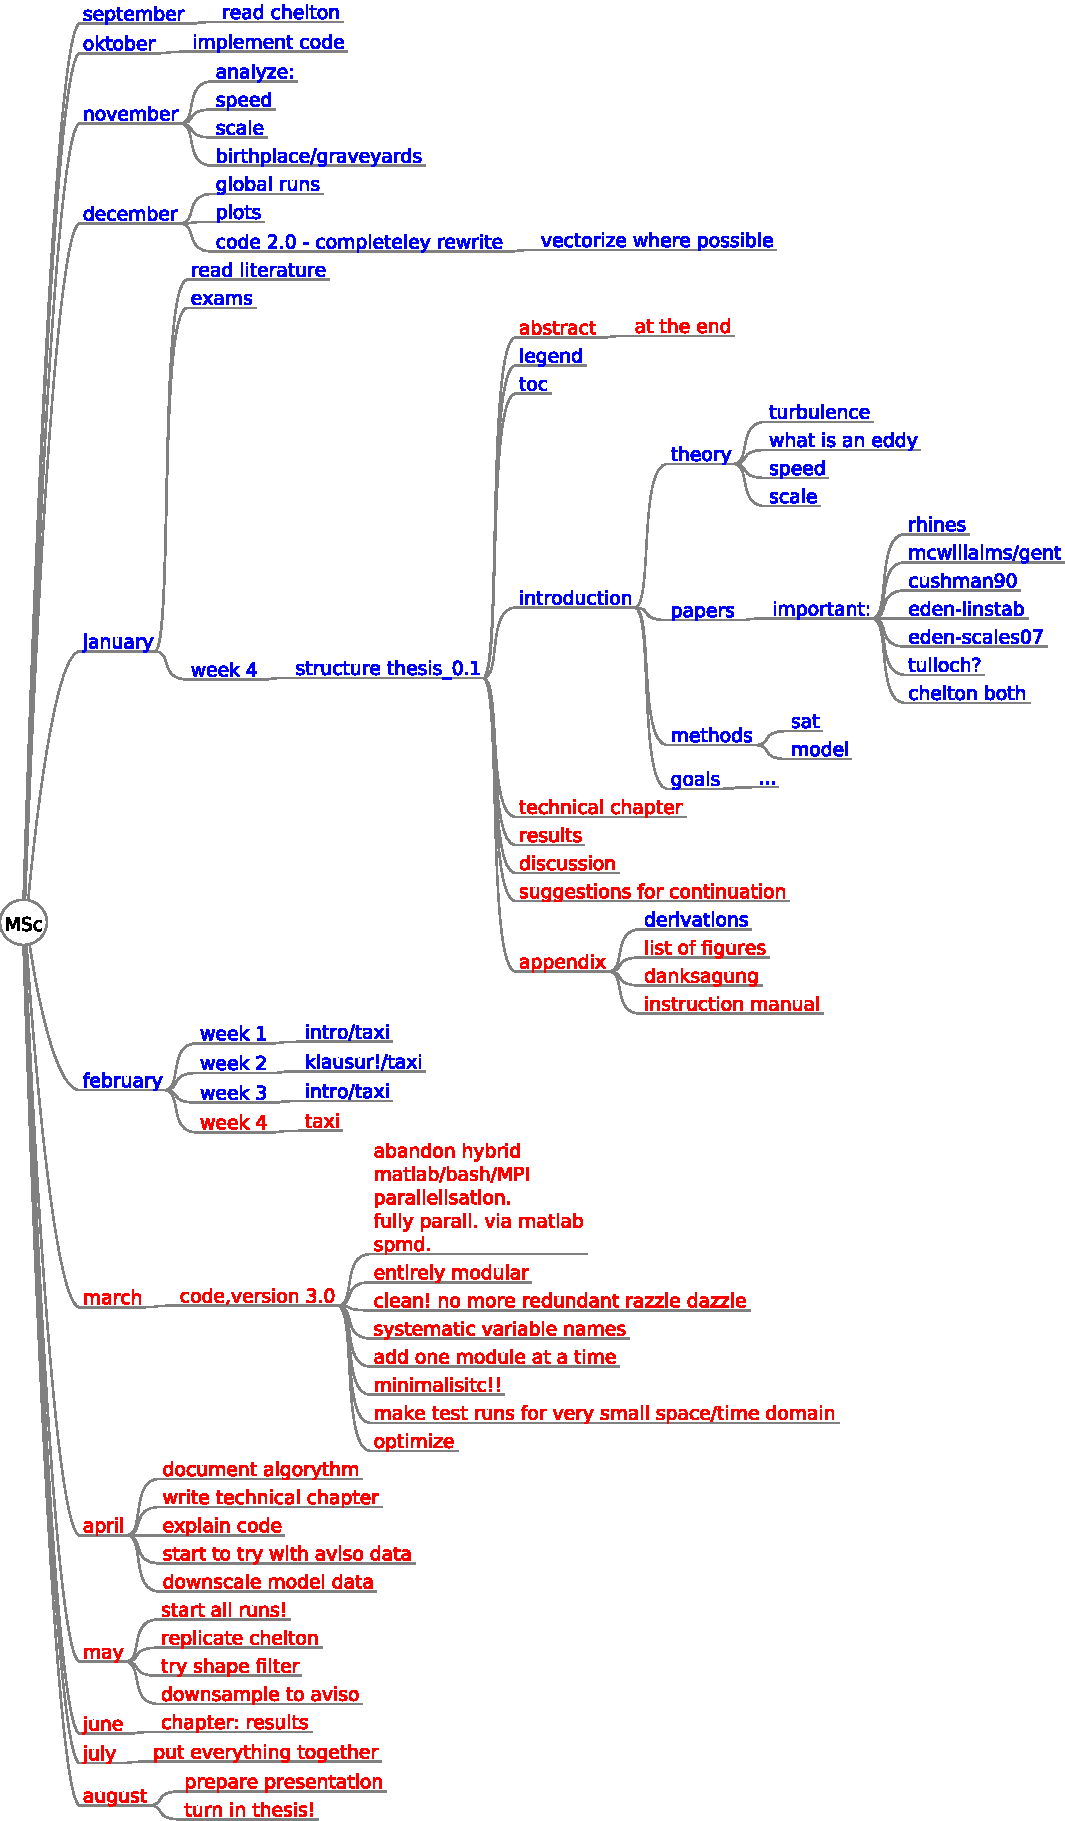
\includegraphics[height=\textheight]{masterplan.pdf}

%\end{figure}

\href{https://drive.google.com/file/d/0B1wN06WMAqAqR180ZnA0S0RqSm8/edit?usp=sharing}{follow this link for up to date mind map}
% \begin{titlepage}
	\vspace*{\fill}
	\begin{center}
		\textsc{\LARGE \univname}\\[1.5cm] % Name of your university/college
		\textsc{\Large Master's Thesis}\\[0.5cm] % Major heading such as course name
		\HRule \\[0.4cm]
		{ \huge \bfseries \ttitle}\\[0.4cm] % Title of your document
		\HRule \\[1.5cm]
		\begin{minipage}{0.4\textwidth}
			\begin{flushleft} \large
				\emph{Author:}\\\textsc{\authornames} % Your name
			\end{flushleft}
		\end{minipage}
		\begin{minipage}{0.4\textwidth}
			\begin{flushright} \large
				\emph{Supervisor:} \\ \textsc{\supname} % Supervisor's Name
			\end{flushright}
		\end{minipage}\\[4cm]
		{\large \today}\\[3cm] % Date, change the \today to a set date if you want to be precise
	\end{center}
	%\vspace*{\fill}
\end{titlepage}

% \begin{abstract}
\todoil{abstract}
will be added last...
\end{abstract}
\newpage

  \tableofcontents
%  \chapter{Legend}
\newpage
  \begin{multicols}{3}

\begin{definition}[Reynolds Number $\mathrm{Re}\unit{\;}$] \label{def:Re}
Compares advection of momentum to frictional acceleration.\\
$\mathrm{Re} = \frac{U L}{\nu}$
 \end{definition}
%###################################%



\begin{definition}[Rossby Number $\Ro \unit{\;}$ ] \label{def:Ro}
Compares advection of momentum to Coriolis acceleration.\\
$\Ro = \frac{U }{f L}$
 \end{definition}
%###################################%



\begin{definition}[Rhines Number $\Rh \unit{\;}$ ]\label{def:Rh}
Ratio of Rhines scale to horizontal scale.\\
$\Rh = \frac{U }{\beta L^2} = \frac{a}{L} \Ro$
  \end{definition}
%###################################%



\begin{definition}[Burger Number $\Bu \unit{\;}$ ]\label{def:Bu}
Ratio of relative vorticity to \textit{stretching} vorticity.\\
$\sqrt{\Bu}=\frac{N H}{f L}=\frac{\mathrm{L_R}}{L}$
 \end{definition}
%###################################%


\begin{definition}[mass $m \unit{kg}$] \label{def:m}
\end{definition}
%###################################%

\begin{definition}[gravitational acceleration $\g \unit{m/s^2}$] \label{def:g}
Value of surface normal component of all body forces.
\end{definition}
%###################################%


\begin{definition}[vorticity $\omega \unit{1/s}$] \label{def:vort}
\end{definition}
%###################################%


\begin{definition}[Buoyancy Vector $\B \unit{1/s^{2}}$] \label{def:B }
$\B= -\frac{ \grad \rho 	\times \grad p}{ \rho^{2}} $
\end{definition}
%###################################%

\begin{definition}[Kinetic Energy per mass $\Ek \unit{m^{2}/s^{2}}$] \label{def:E_k}
\end{definition}
%###################################%

\begin{definition}[Mechanical Energy per mass $\Ek \unit{m^{2}/s^{2}}$] \label{def:E_m}
Sum of kinetic and potential Energy.
\end{definition}
%###################################%


\begin{definition}[Rossby Radius $\mathrm{L_{R}} \unit{m}$ ]\label{def:Lr}
The \textit{geostrophic wavelength}.
$\mathrm{L_{R}} = c/f $
 \end{definition}
%###################################%



\begin{definition}[Steering Level $z_S$]\label{def:steer}
The critical depth where the real part of the Doppler shifted phase
speed $c_S(z_S)=\real{c(z)}-u(z)=0$ vanishes. \Ie the depth where the Doppler shift
creates a standing wave, causing the disturbances to grow in place instead of
spreading in space, analogous to a \textit{supersonic bang}.
 \end{definition}
%###################################%



\begin{definition}[Rhines Scale $\mathrm{L_{\beta}} \unit{m}$ ]\label{def:Lb}
Scale at which earth's sphericity becomes important.\\
$\mathrm{L_{\beta}}^2 = \frac{U}{\beta} $
 \end{definition}
%###################################%



\begin{definition}[Gravity Wave Phase Speed $\mathrm{c} \unit{m/s}$ ]\label{def:c}
$\mathrm{c}  = \sqrt{g'H} $
 \end{definition}
%###################################%



\begin{definition}[Reduced Gravity $g'(x,y,z) \unit{m/s^{2}}$ ]\label{def:gr}
In the layered model $g'=g \frac{\delta \rho}{\rho_0} = N^{2}h$
 \end{definition}
%###################################%



\begin{definition}[Surface/interface Displacement $\eta(x,y)
\unit{m}$]\label{def:eta}
 \end{definition}
%###################################%



\begin{definition}[Brunt V\"ais\"al\"a frequency $N \unit{1/s}$]\label{def:BVf}
$N^2=g/\rho_0 \dpr{\rho}{z}$
 \end{definition}
%###################################%



\begin{definition}[Mean Layer thickness $H \unit{m}$]\label{def:H}
 \end{definition}
%###################################%



\begin{definition}[Layer Thickness/physical height of an isopycnal surface $h(x,y,t) \unit{m}$/$h(x,y,\rho,t) \unit{m}$]\label{def:h}
$h = H+\eta$ (in the layered model)
 \end{definition}
%###################################%



\begin{definition}[Planetary Vorticity $\Omega \unit{1/s}$]\label{def:Omega}
$\Omega=4\pi/\mathrm{day}_{fix\star}$
 \end{definition}
%###################################%



\begin{definition}[Latitude $\phi \unit{\mathrm{rad}}$]\label{def:phi}
 \end{definition}
%###################################%



\begin{definition}[Earth's Radius $a \unit{m}$]\label{def:a}
 \end{definition}
%###################################%



\begin{definition}[Surface-Normal Planetary Vorticity Component $\vec{f}
\unit{1/s}$]\label{def:f}
$\vec{f}=\f \vec{z}=\Omega \sin \phi \vec{z}$
 \end{definition}
%###################################%



\begin{definition}[Change of Planetary Vorticity with Latitude
$\beta \unit{1/ms}$]\label{def:beta}
$\dfdy=\dpr{\f}{y}=\Omega/a \cos \phi$
 \end{definition}
%###################################%


\begin{definition}[Okubo-Weiss Parameter
$\okubo \unit{1/s^2}$]\label{def:okubo}
$\okubo=divergence^2+ stretching^2+ shear^2- vorticity^2$.\\
A negative value indicates vorticity dominated motion, whereas a positive value
indicates deformation.
\end{definition}
%###################################%

\begin{definition}[Sea Surface Height
\SSH $\unit{m}$]\label{def:SSH}
 \end{definition}
%###################################%

\begin{definition}[Isoperimetric Quotient
$\IQ \unit{\;}$]\label{def:IQ}
$\IQ=A/A_{c}=\frac{A}{\pi r^2_{c}}=\frac{4 \pi A}{U^2} \le 1$.\\
The ratio of a ring's area to the area of a circle with equal circumference.
 \end{definition}
%###################################%

\begin{definition}[Gaussian radius
$\rG \unit{m}$]\label{def:rG}
$ \left( H-a \right) = H \exp \left( -\frac{A}{2 \pi \rG^2}  \right)$.\\
Twice the Gaussian standard-deviation. \\
$a$: amplitude\\
$H$: Gaussian amplitude\\
$A$: determined area\\
 \end{definition}
%###################################%


\end{multicols}


% 
% 
% 
% 
% 
% %%####################################################################
% %%####################################################################
% 
% %####################################################################
% 
  \mainmatter
  \setstretch{0.9}
  \newgeometry{left=1cm, right=4cm, top=2cm, bottom=2cm}
  \pagestyle{fancy} % Return the page headers back to the "fancy" style
% \chapter{Introduction}
% \section{Theory}
%%--------------------------------------------------------------------
\label{chap:intro}


\begin{wrapfigure}[20]{r}{0.5\textwidth}
\vspace{-5mm}
\begin{center}
  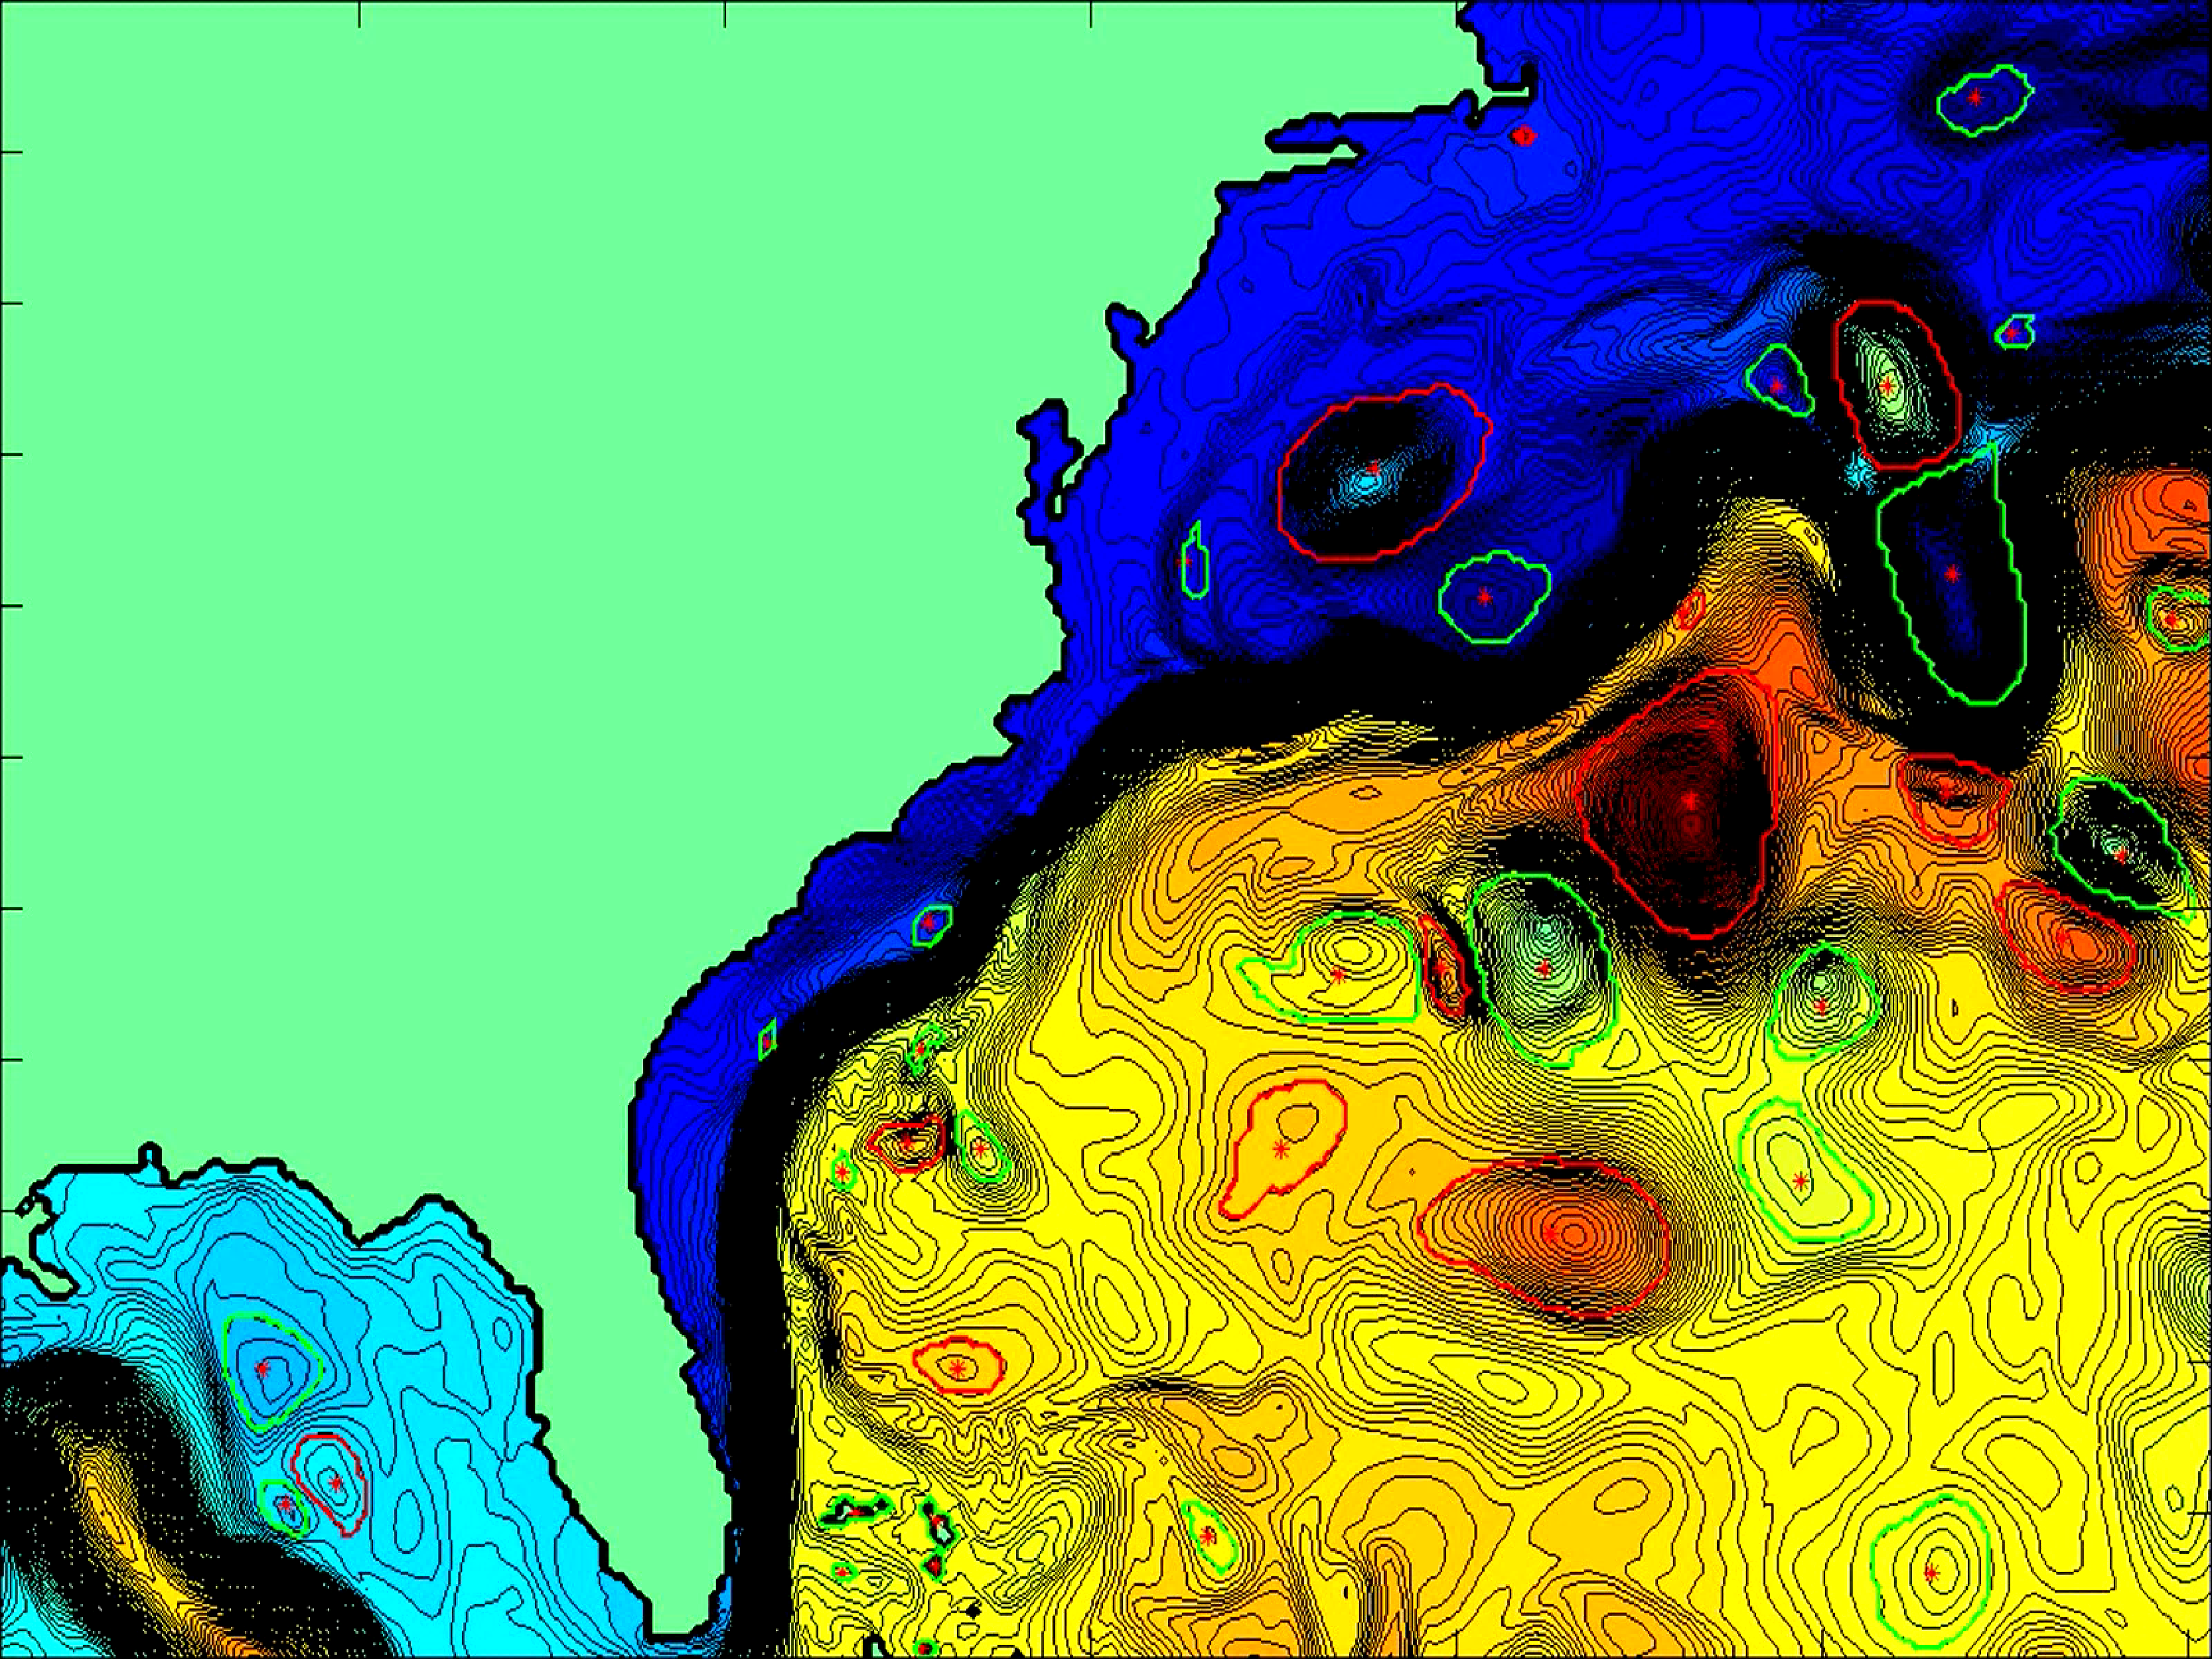
\includegraphics[width=.5\textwidth]{GS.pdf}
\caption{Animation snapshot of early test run. Shown is SSH with detected eddies indicated.}
\end{center}
\vspace{-15mm}
\end{wrapfigure}


\paragraph{This}chapter discusses the theory of meso-scale turbulence and parametrizations thereof.
Geostrophic turbulence is typically characterized by rather stable, circular, coherent pressure anomalies, that rotate fluid around in a vortex in
quasi-geostrophic equilibrium. These entities can persist for long periods of time in which they often travel distances on the order of hundreds of kilometers
zonally. The fact that baroclinic instability forms these vortices instead of leading to a cascade to ever smaller scales ,as would be expected from chaotic
turbulence, is a direct consequence of the inverse energy cascade of 2-dimensional motion. For a discussion of this phenomenon see appendix
\ref{chap:turbu_categories}. The atmospheric analog are storms and high-pressure systems, yet with much less difference between high- and low-pressure systems due to
a smaller centrifugal force \ie smaller Rossby number. These quasi-geostrophic, meso-scale vortices, from here on called eddies \footnote{For a discussion of
the different types of vortices in the ocean see appendix \ref{chap:eddy_cat}}, are immediately visible on
SSH maps. Yet, it is difficult to physically \emph{define} an eddy in terms of oceanographic variables. The transition from meandering jets or other undeveloped
baroclinic turbulence is not very sharp. Eddies also sometimes merge or split or collectively form rifts and valleys in SSH. detecting them on one snapshot
automatically via an algorithm is therefore not trivial. Further problems arise when the algorithm is also supposed to track them. Their shear abundance at any
given time inevitably creates ambiguities between time steps. It is therefore necessary to set up a clear, unambiguous, sufficient (in the mathematical sense)
definition.\\

\subsection{Detection methods} \label{subsec:detectmethods}
\begin{itemize}
	\item
	One way to find an eddy in SSH-data is to simply scan for closed contours at different values for $\vec{z}$ and then subject found entity to a series of necessary tests. Only if all criteria are met is an eddy found. This method was first used by \cite{Chelton2011} and turned out to be the simplest yet most effective method, at least for satellite SSH data. Therefore, as a starting point, this method will be adopted and should also serve as a general definition of what will be referred to as an \textit{eddy} hereafter\footnote{The vortices will have names deviant from \textit{eddy} where these criteria are altered.}.\\
	\citeauthor{Chelton2011} set the following threshold criteria for his algorithm:
\begin{enumerate}
\item
The SSH values of all of the pixels are above (below) a given SSH threshold for anticyclonic (cyclonic) eddies.
\item
There are at least \textit{[threshold]} pixels and fewer than \textit{[threshold]} pixels comprising the connected region.
\item
There is at least one local maximum (minimum) of SSH for anticyclonic (cyclonic) eddies.
\item
 The amplitude of the eddy is at least \textit{[threshold]}.
\item
The distance between any pair of points within the connected region must be less than \textit{[threshold]}.
\end{enumerate}

\item
Another frequently used method do define an eddy makes use of the strain tensor $\ten{T}$\derref{der:okubo}. The trace of the strain tensor squared includes
valuable information about the dynamics of the velocity field. Namely
%%....................................................................
\begin{equation}\begin{split}
	2\mathrm{O_w}=\tr{\ten{T}^2}
	=
	divergence^2
	+ stretching^2
	+ shear^2
	 - vorticity^2 \\
\end{split}\end{equation}
%%....................................................................
which reduces to $\mathrm{O_w}= \left(\partial_x u\right)^2+2 \partial_y u \partial_x v$ in 2 dimensions. This is called the
Okubo\footnote{\cite{Okubo1970}}-Weiss-Parameter. It is a useful tool to determine whether the field has parabolic, vorticity dominated character, or whether
deformation dominates giving hyperbolic character. An area of large negative values indicates high enstrophy density compared to gradients of kinetic energy,
thus indicating little friction paired with high momentum \ie a coherent, angular-momentum-conserving entity. Positive values on the other hand indicate
incoherent deformation.\\ As genius as this parameter seems, it turns out that using it to identify eddies is often not the best solution.
\citeauthor{Chelton2011} names 3 major drawbacks:
\begin{itemize}
	\item
	\textit{ No single threshold value for $\mathrm{O_W}$ is optimal for the entire World Ocean. Setting the threshold too high can result in failure to identify small eddies, while a threshold that is too low can lead to a definition of eddies with unrealistically large areas that may encompass multiple vortices, sometimes with opposite polarities. }
	\item
	$\mathrm{O_W}$ is highly susceptible to noise in the SSH field. Especially when velocities are calculated from geostrophy, the sea surface has effectively
been differentiated twice and then squared, exacerbating small incontinuities in the data.
	\item
	\textit{The third problem with the W-based method is that the interiors of eddies defined by closed contours of W do not generally coincide with closed contours of SSH. The misregistration of the two fields is often quite substantial. }
\end{itemize}
It is hence only logical to scan for closed contours of SSH directly (as was done so by \citeauthor{Chelton2011}).

\item
\todo[inline]{vector based detection etc}



\end{itemize}








\subsection{Eddy Drift Speeds}\label{subsec:speeds}
%%%--------------------------------------------------------------------

Intuitively any translative motion of a vortex should stem from an asymmetry of forces as in an imperfectly balanced gyroscope wobbling around and translating across the table. The main effects that cause a quasi-geostrophic ocean eddy to translate laterally can easily be explained heuristically.
\begin{description}
\litem{Lateral Density Gradient}{speed_dens}
Consider a mean layer-thickness gradient $\dpr{h}{x}>0$ somewhere in the high northern latitudes and a geostrophic, positive density anomaly within that layer.
In other words a high-pressure vortex or an anti-cyclonic eddy with length scale $L\approx \mathrm{L_{R}}$. Hence a vorticity budget dominated by advection of
relative vorticity and vortex stretching. Consider a parcel of water adjacent to the eddy on its eastern flank. Due to the eddy's negative vorticity, the parcel
will be advected west into shallower layer-thickness where it will be squeezed vertically and acquire negative relative vorticity via term $C$ in \eqref{eq:vort7}.
Analogously a parcel of initially zero $\vec{\omega}$ on the eddy's western flank will be transported east, stretched and thereby acquire positive relative
vorticity. The result is that the eddy will be shoved south from both zonal flanks. Note that the rotational sense of the eddy is irrelevant here. The drift
direction is dictated by the sign of $f$. Hence eddies in the
northern hemisphere will be pushed along gradients with the shallower water always on their right and vice versa on the southern hemisphere.
\litem{\textit{Planetary Lift}}{speed_planlift}
Assume now that $\beta L$ be comparable or larger even than $f_{0}-\omega$ from the previous example. Then, all fluid adjacent to the eddy on its northern and southern flanks will be transported meridionally, thereby be tilted with respect to $\Omega$ and hence acquire relative vorticity to compensate. All fluid transported north will balance the increase in planetary vorticity with a decrease in relative vorticity and vice versa for fluid transported south. This is again independent of the eddy's sense and in this case also independent of hemisphere since $\dpr{f}{y}=\beta>0$ for all latitudes. The result is that small negative vortices to the northern and small positive vortices to the southern flank of eddies will push them west.
\litem{Eddy-Internal $\beta$-Effect}{speed_beta}
In the later case clearly particles within the vortex undergo a change in planetary vorticity as well. Or from a different point of view, since $U \sim \grad p/f  $, and noting that the pressure gradient is the driving force here and hence fix at first approximation, particles drifting north will decelerate and those drifting south will accelerate. In order to maintain mass continuity, the center of volume will be shifted west for an anti-cyclone and east for a cyclone. Another way to look at it is to note that the only way for the discrepancy in Coriolis acceleration north and south, whilst maintaining constant eddy-relative particle speed, is to superimpose a zonal drift velocity so that net particle velocities achieve symmetric Coriolis acceleration.
\end{description}

%{\color{red} equations to follow \cite{Cushman-Roisin1990} \cite{VanLeeuwen2007}}
\newpage

%%%--------------------------------------------------------------------

\subsection{The Integral Length Scale of Turbulence}
%%--------------------------------------------------------------------
\paragraph{This} section is intended to shed light on the benefits of exact determinations of ocean-eddy-\textit{scales}. That is, their horizontal extent \ie
their diameter or \textit{wavelength}.
%%%####################################################################
%%%####################################################################
\paragraph{Just}~like the \emph{eddy} itself, its scale is rather vague and difficult to define. What physical parameter defines the outer edge of a seamless, smooth vortex? If the eddy is detected as done by \cite{Chelton2011}, \ie closed contours of SSH the interior of which fulfilling certain criteria, the measured perimeter may jump considerably from one time step to the next. An incremental difference in the choice of $z$ might translate to a perimeter outlining twice the  difference in area, especially when SSH gradients are small.\\
Another possibility is to define an amplitude first, then assume a certain shape \eg Gaussian, and then infer the radius indirectly. The obvious problem with this approach would be to properly define the amplitude.\\
The most physically sound method would have to be one depending on the eddy's most defining physical variable, that is unambiguously determinable from SSH. The geostrophic velocities. \cite{Chelton2011}, as with everything else, tried all methods but also conclude that the later is the most adequate one. \footnote{See Chapter }\todoil{ref to technical chapter}.

%%
%%%####################################################################
%%%####################################################################
%
\begin{wrapfigure}{r}{0.5\textwidth}
  \begin{center}
\includegraphics[width=.5\textwidth]{SSHB.pdf}
  \end{center}
  \caption{top: Stommel's equation $\mathcal{F}_{bottom}-\mathcal{F}_{surface}= -v\beta$ with constant eddy viscosity. bottom: Parallel Ocean Program eddy-resolving model snapshot with SSH mean of one year subtracted. }
\end{wrapfigure}


\paragraph{Construed} as an integral length scale of turbulence \ie as the distance at which the auto-correlation of particles reaches zero, the \emph{eddy-scale} turns out to be of fundamental relevance for attempts to parametrize geostrophic turbulence.\\
General circulation models ($\order{2}$km) as they are used in \eg climate forecasts are too coarse to resolve meso-scale ($\order{1}$km) turbulence. Even if the Von-Neumann-condition were ignored and a refinement were desired horizontally only, a leap of one order of magnitude would cause an increase in calculation time of factor \footnote{With the Moore's-Law-type exponential growth in FLOP/S of the last 22 years for supercomputers ($\lg(x)\sim 3/11 a$) a factor $100$ interestingly translates to only $a=22/3\approx 7$ years...} $x=100$.  The effects of the nonlinear terms therefore have to be somehow articulated in an integral sense for the large grid-boxes in the model.
A common approach is to assume that \textit{eddy kinetic energy} $\ol{ \vec{u}'\vec{u}'}$ and \textit{eddy potential energy} $\ol{  w'\rho'}$, akin to diffusive
processes \footnote{In analogy to Fick's first law of diffusion}, are proportional to the gradient of $\ol{u}$ respective $\ol{b}$
(down-gradient-parametrization \footnote{\ie Reynolds averaging}) \citep*{olbers2012ocean}, which leads to the problem of finding expressions for the
\textit{turbulent diffusivities} \ie the rate at which gradients are diffused by turbulence. This parameter is by no means constant, instead it can span
several orders of magnitude, itself depending on the strength of turbulence-relevant gradients, and sometimes even assuming negative values
\citep{eden2008towards}. Precise knowledge of the integral length scale and the physics that set it is hence vital for attempts to analyze and set values for
eddy diffusivites and turbulence parametrizations in general.


%\paragraph{Eddy Diffusivities} For simplicity assume full incompressibility and a variable density $\rho(T)$, that is linearly dependent on temperature only and that there be some radiative surface flux $J^{rad}$ for $T$, hence also for $\rho$. Further consider kinetic energy being burned to heat on molecular scales \ie Joule heating, creating another positive source of $T$ thus $\rho$. \derref{der:FIELDSDER}

%%%....................................................................
%\begin{subequations} \label{eq:inhomo_fin}
%\begin{align}
	%\dpr{\ol{\vec{u}_h}}{t}
	%+
	%\ol{ \dpr{w'\vec{u}_h'}{z}}
	%+
	%f \vec{k} \times \ol{\vec{u}_h}
	%&=
	%0 \\
		 %%%--------------------------------------------------------------------
	 %\dpr{\ol{\rho}}{t}
	 %&=
	 %-\dpr{}{z}
	 %\left(
%\ol{  w'\rho'}
%-\ol{\vec{J}}_{rad}
%+   \kappa \dpr{ \ol{\rho}}{z} \right)
%\end{align}
%\end{subequations}
%%%....................................................................
%\todoil{introduce buoyancy instead rho- for eq. of state}
%If the aim was to solve \eqsref{eq:inhomo_fin} numerically for the mean quantities, parametrizations for the \textit{eddy kinetic energy}-term $\ol{ w'\vec{u}_h'}$ and the \textit{eddy potential energy}-term \footnote{$\ol{  w'\rho'}$ is an exchange term between potential and kinetic energy} $\ol{  w'\rho'}$ would have to be found. A common approach is to assume that the turbulent energy, akin to diffusive processes\footnote{In analogy to Fick's first law of diffusion}, is proportional to the gradient of $\ol{u}$ respective $\ol{b}$  (down-gradient-parametrization) \citep*{olbers2012ocean}.
%%%....................................................................
%\begin{subequations} \label{eq:downgrad}
%\begin{align}
%\ol{ w'\vec{u}_h'}
%&=
%-K_u \dpr{\ol{\vec{u}}}{z} \\
  %%%--------------------------------------------------------------------
 %\ol{  w'b}
 %&=
  %-K_{b} \dpr{\ol{b}}{z}
%\end{align}
%\end{subequations}
%%%....................................................................
%which leads to the problem of finding expressions for the turbulent diffusivities $K$. Heuristic considerations \citep{olbers2012ocean} suggest that $K \sim UL \sim \sqrt{E_t} L$ with the turbulent kinetic energy $E_t \sim \ol{u'u'}$. Assuming for now that the characteristic length scale $L$ is known and that the proportionality factors $c$ could be determined empirically, we still need to find an expression for $\Ek$. With $\star$ for either $u$ or $b$:
%%%....................................................................

%\begin{align}
%K_{\star}
%&=
%c_{\star} \sqrt{E_t} L
%\end{align}

%%%....................................................................
%Unfortunately the $E_t$-equation is itself full of unknowns \derref{der:TURBKINDER}.
%\begin{align}
	%\dpr{E_t}{t}
	%+
	%\ol{w} \dpr{E_t}{z}
	%&=
	%\dpr{\vec{\psi}}{z}
	%-
	%\ol{ \vec{u}_h' w'\dpr{\ol{\vec{u}}_h}{z}}
	%+
	%\ol{b'w'}
	%-
	 %\nu \ol{  \left(\grad \vec{u}' \right)^2	}  \label{eq:TurbKinFinHorHomoText}
%\end{align}
%\cite{Gaspar1990} model the flux-term as \citep{olbers2012ocean}.
%%%....................................................................
%\begin{align}
%\vec{\psi}
%&=
%c_e \sqrt{ E_t} L \dpr{E_t}{z}
%\end{align}
%%%....................................................................
%The $-\ol{ \vec{u}_h' w'\dpr{\vec{\ol{u}}_h}{z}}$-term draws energy off the mean-energy-gradient. Using again down-gradient parametrization: $\ol{\vec{u}_h' w'}=-K_u \dpr{\vec{u}_h}{z}$. The last term represents dissipation and can be expressed via the Kolmogorov-type parametrization $\nu\ol{  \left(\grad \vec{u}' \right)^2	} =\epsilon =c_{\epsilon} \frac{E_t^{3/2}}{L}$. Hence:
%\begin{align}
	%\dpr{E_t}{t}
	%+
	%\ol{w} \dpr{E_t}{z}
	%&=
	%\dpr{}{z}\left(c_e  \sqrt{ E_t} L \dpr{E_t}{z}\right)
	%-
	%K_u  \left( \dpr{\ol{\vec{u}}_h}{z} \right)^2
	%-
	%K_{b} \dpr{\ol{b}}{z}
	%-
	%c_{\epsilon} \frac{E_t^{3/2}}{L} \label{eq:EtFin}
%\end{align}
%\eqref{eq:EtFin} could now be solved for $E_t$. All other variables are either from the mean state, coefficients or the integral length-scale $L$.\\
%The conclusion of this section is therefor, that a precise knowledge of the characteristic integral length scale of the turbulent motion is a fundamental
ingredient to parametrizations of turbulence in \eg non-eddy-resolving climate models.

%%--------------------------------------------------------------------


%%--------------------------------------------------------------------
\section{Important Papers}
%%--------------------------------------------------------------------


\subsection{\citealt{Rhines2006}}\label{sec:hist_rhines}
Rhines investigated the effect of the $\beta$-plane on the inverse energy cascade of quasi-2-dimensional atmospheric and oceanic turbulence. At constant $f$, energy should be cascaded to ever-larger scales until halted by the scale of the domain. This is clearly not the case, as no storm has ever grown to global scale. The presence of a meridional restoring force creates a critical scale beyond which the \textit{turbulent migration of the dominant scale nearly ceases \ldots}. Instead, Rossby waves are excited which would theoretically eventually give way to alternating zonal jets of width $\mathrm{L_{\beta}}$. This scale was later coined the Rhines Scale.




\subsection{\citealt{Cushman-Roisin1990}}\label{sec:hist_cush}
\cite{Bjerknes1944} already noted that the $\beta$-effect causes a mass-imbalance in planetary vortices that, if not met by an asymmetry in shape must lead to westward propagation. \cite{Nof1981} derived that the $\beta$-effect results in a net meridional force on the integrated mass of the vortex, which in balance with the Coriolis acceleration shoves cyclones eastward and anti-cyclones westward. They also explained how displaced water outside the eddy's perimeter causes a much stronger westward component, with the result that all eddies propagate westward irrespective or rotational sense. The westward drift was also derived in various forms by
\eg \cite{flierl1984rossby,matsuura1982evolution}. \\
\citet{Cushman-Roisin1990} put it all into a less restricted uniform formalism by scaling the terms in the one-layer primitive equations by their respective dimensionless numbers. By integrating the interface-displacement caused by the eddy over the eddy's domain and applying mass continuity they derived for the location $(X,Y)$ of an eddy's centroid\footnote{$\intms{}\equiv \intm{}$}:
%%....................................................................
\begin{equation}\begin{split}
	\Pi X_{tt} - Y_t
	%&=
	%\frac{\Bu \Ro }{\Rh \Pi} \intms{yv}
	%+
	%\frac{\Ro^2 }{\Rh \Pi} \intms{y\eta v}\\
	%%--------------------------------------------------------------------
	&=
	\Lr T \beta     \intms{yv}
	+
	L\frac{  \beta  }{ f   } \intms{y\eta v}\\
	%%--------------------------------------------------------------------
	\Pi Y_{tt} - X_t
	%&=
	%-\frac{\Bu \Ro }{\Rh \Pi } \intms{yu}
	%-
	%\frac{\Ro^2 }{\Rh \Pi} \intms{y\eta u}\\
	%%--------------------------------------------------------------------
	&=
	-\Lr T \beta   \intms{yu}
	-
	L\frac{  \beta  }{ f   }  \intms{y\eta u} 	  \label{eq:cush1}
\end{split}\end{equation}
%....................................................................
where $\Pi=1/f_0T$.\\
 Hence, independent of balance of forces the eddy's center of mass describes inertial oscillations \footnote{compare to \textit{harmonic oscillator}} on the $f$-plane, even in the absence of $\beta$.
Using geostrophic values for $\vec{u}$ and returning to dimensional variables \eqref{eq:cush1} can be cast into:
%%%....................................................................
%\begin{equation}\begin{split}
	%X_t
	%&=
	%-\frac{\Bu \Ro f T}{\Rh} \intms{\eta}
	%-\frac{\Ro^2 f T}{\Rh} \intms{\eta^2}
	%+\order{\frac{\Bu \Ro f T}{\Rh},\left( fT \right)^{-2}}
%\end{split}\end{equation}
%%%%....................................................................
%%....................................................................
\begin{equation}\begin{split}
	X_t
	&=
	\frac{\omega_{long}}{k} \left(1 +\frac{1}{H} \frac{ \int  \eta^2 \; \mathrm{d}A	}{2\mathrm{V_e}} \right)
	%+\order{\Lr   T\beta ,\Pi}
\end{split}\end{equation}
%%....................................................................

The first term represents the \ref{speed_planlift} from \ref{subsec:speeds}, whereas the second term represents the \ref{speed_beta}. Note that the first term is always westwards, while the second has sign of $-\eta$, \ie westward for anti-cyclones and eastward for cyclones and that the first is always larger than the second.
\todoil{\cite{VanLeeuwen2007} for derivation if time}



\subsection{Early Altimeter Data}\label{sec:hist_killworth}
The advent of satellite altimetry, which Walter Munk called \textit{the most successful ocean experiment of all time \citep{Munk2002}}, finally allowed for
global-scale experimental investigations of oceanic planetary phenomena on long time- and spatial scales. Among others,
\cite{matano1993seasonal,cipollini1997concurrent,le1993sea} were the first to use satellite-data to present evidence for the existence of Rossby waves and their
westward-migration in accord with theory. Surprisingly all of the observations found the phase speeds to be $1$ to $1.5$ times larger than what theory
predicted. Several theories to explain the discrepancy were presented. \Eg \cite{Killworth1997a} argued that the discrepancy was caused by
mode-2-east-west-mean-flow velocities. Interestingly it appears that hitherto, the relevant altimeter signal was mainly associated with linear waves.
Non-linearities are rarely mentioned in the papers of those years. Probably simply due to the fact that the turbulent character of much of the
meso-scale variability was still obscured by the poor resolution of the first altimeter products.



\subsection{\cite{Killworth1997a,Chelton2007,Chelton2011}}\label{sec:hist_chelton}
From the beginning of satellite altimetry \citeauthor{Chelton2011} have continuously invested tremendous effort to thoroughly analyze the data in terms of
Rossby waves and geostrophic turbulence. At the time of their \citeyear{Killworth1997a} paper only 3 years of Topex/Poseidon data alone had been available,
which led them to interpret the data mainly in terms of Rossby waves. Once the merged Aviso T/P and ERS 1/2 \todoil{ref} was released 7 years later,
\citeauthor{Chelton2007} presented a new analysis that was based on an automated eddy-tracking algorithm using the geostrophic Okubo-Weiss parameter
\footnote{see section \ref{subsec:detectmethods}}\derref{der:okubo}. For the first time Satellite data was sufficiently fine resolved to unveil the dominance of \textit{blobby
(sic) structures rather than latitudinally $\beta$-refracted continuous crests and troughs} that had hitherto been assumed to characterize the large scale SSH
picture. They presented results of a refined algorithm in their \citeyear{Chelton2011} paper, in
which they abandoned the Okubo-Weiss concept and instead identified eddies via closed contours of SSH itself \footnote{note that geostrophic $\mathrm{O_W}$ is a
second derivative of SSH and thus exacerbates noise in the SSH data.}. Among their most significant findings is the conclusion that on the one hand, the vast
majority of extra-tropical west-ward propagating SSH-variability consists of coherent, isolated, non-linear, meso-scale eddies, whilst on the other hand, these
eddies propagate about 25\% slower \footnote{pointing to dispersion.} than small amplitude features of larger lateral scale, that are difficult to separate from
the data and are assumed to obey linear Rossby wave theory. \todoil{rephrase} Apart from this they find little evidence for any dispersion in the signal,
neither do they find evidence for significant meridional propagation, as should be found for Rossby waves. In agreement with \cite{rhines1979theoretical}, they
find this eddy-dominated regime to fade in vicinity of the equator,
giving way to the characteristic Rossby-wave profile. Almost all of their eddies propagate westwards. Those that are advected eastwards by \eg the ACC show significantly shorter life-times than those that are not. For more detail on their results and a discussion of the limitations of eddy-tracking via satellites see section \ref{sec:satvsmod}.

%%--------------------------------------------------------------------
\section{Methods}
%%--------------------------------------------------------------------

\subsection{Satellite vs Model Data} \label{subsec:satvsmod}




\begin{wrapfigure}[50]{r}{0.25\textwidth}

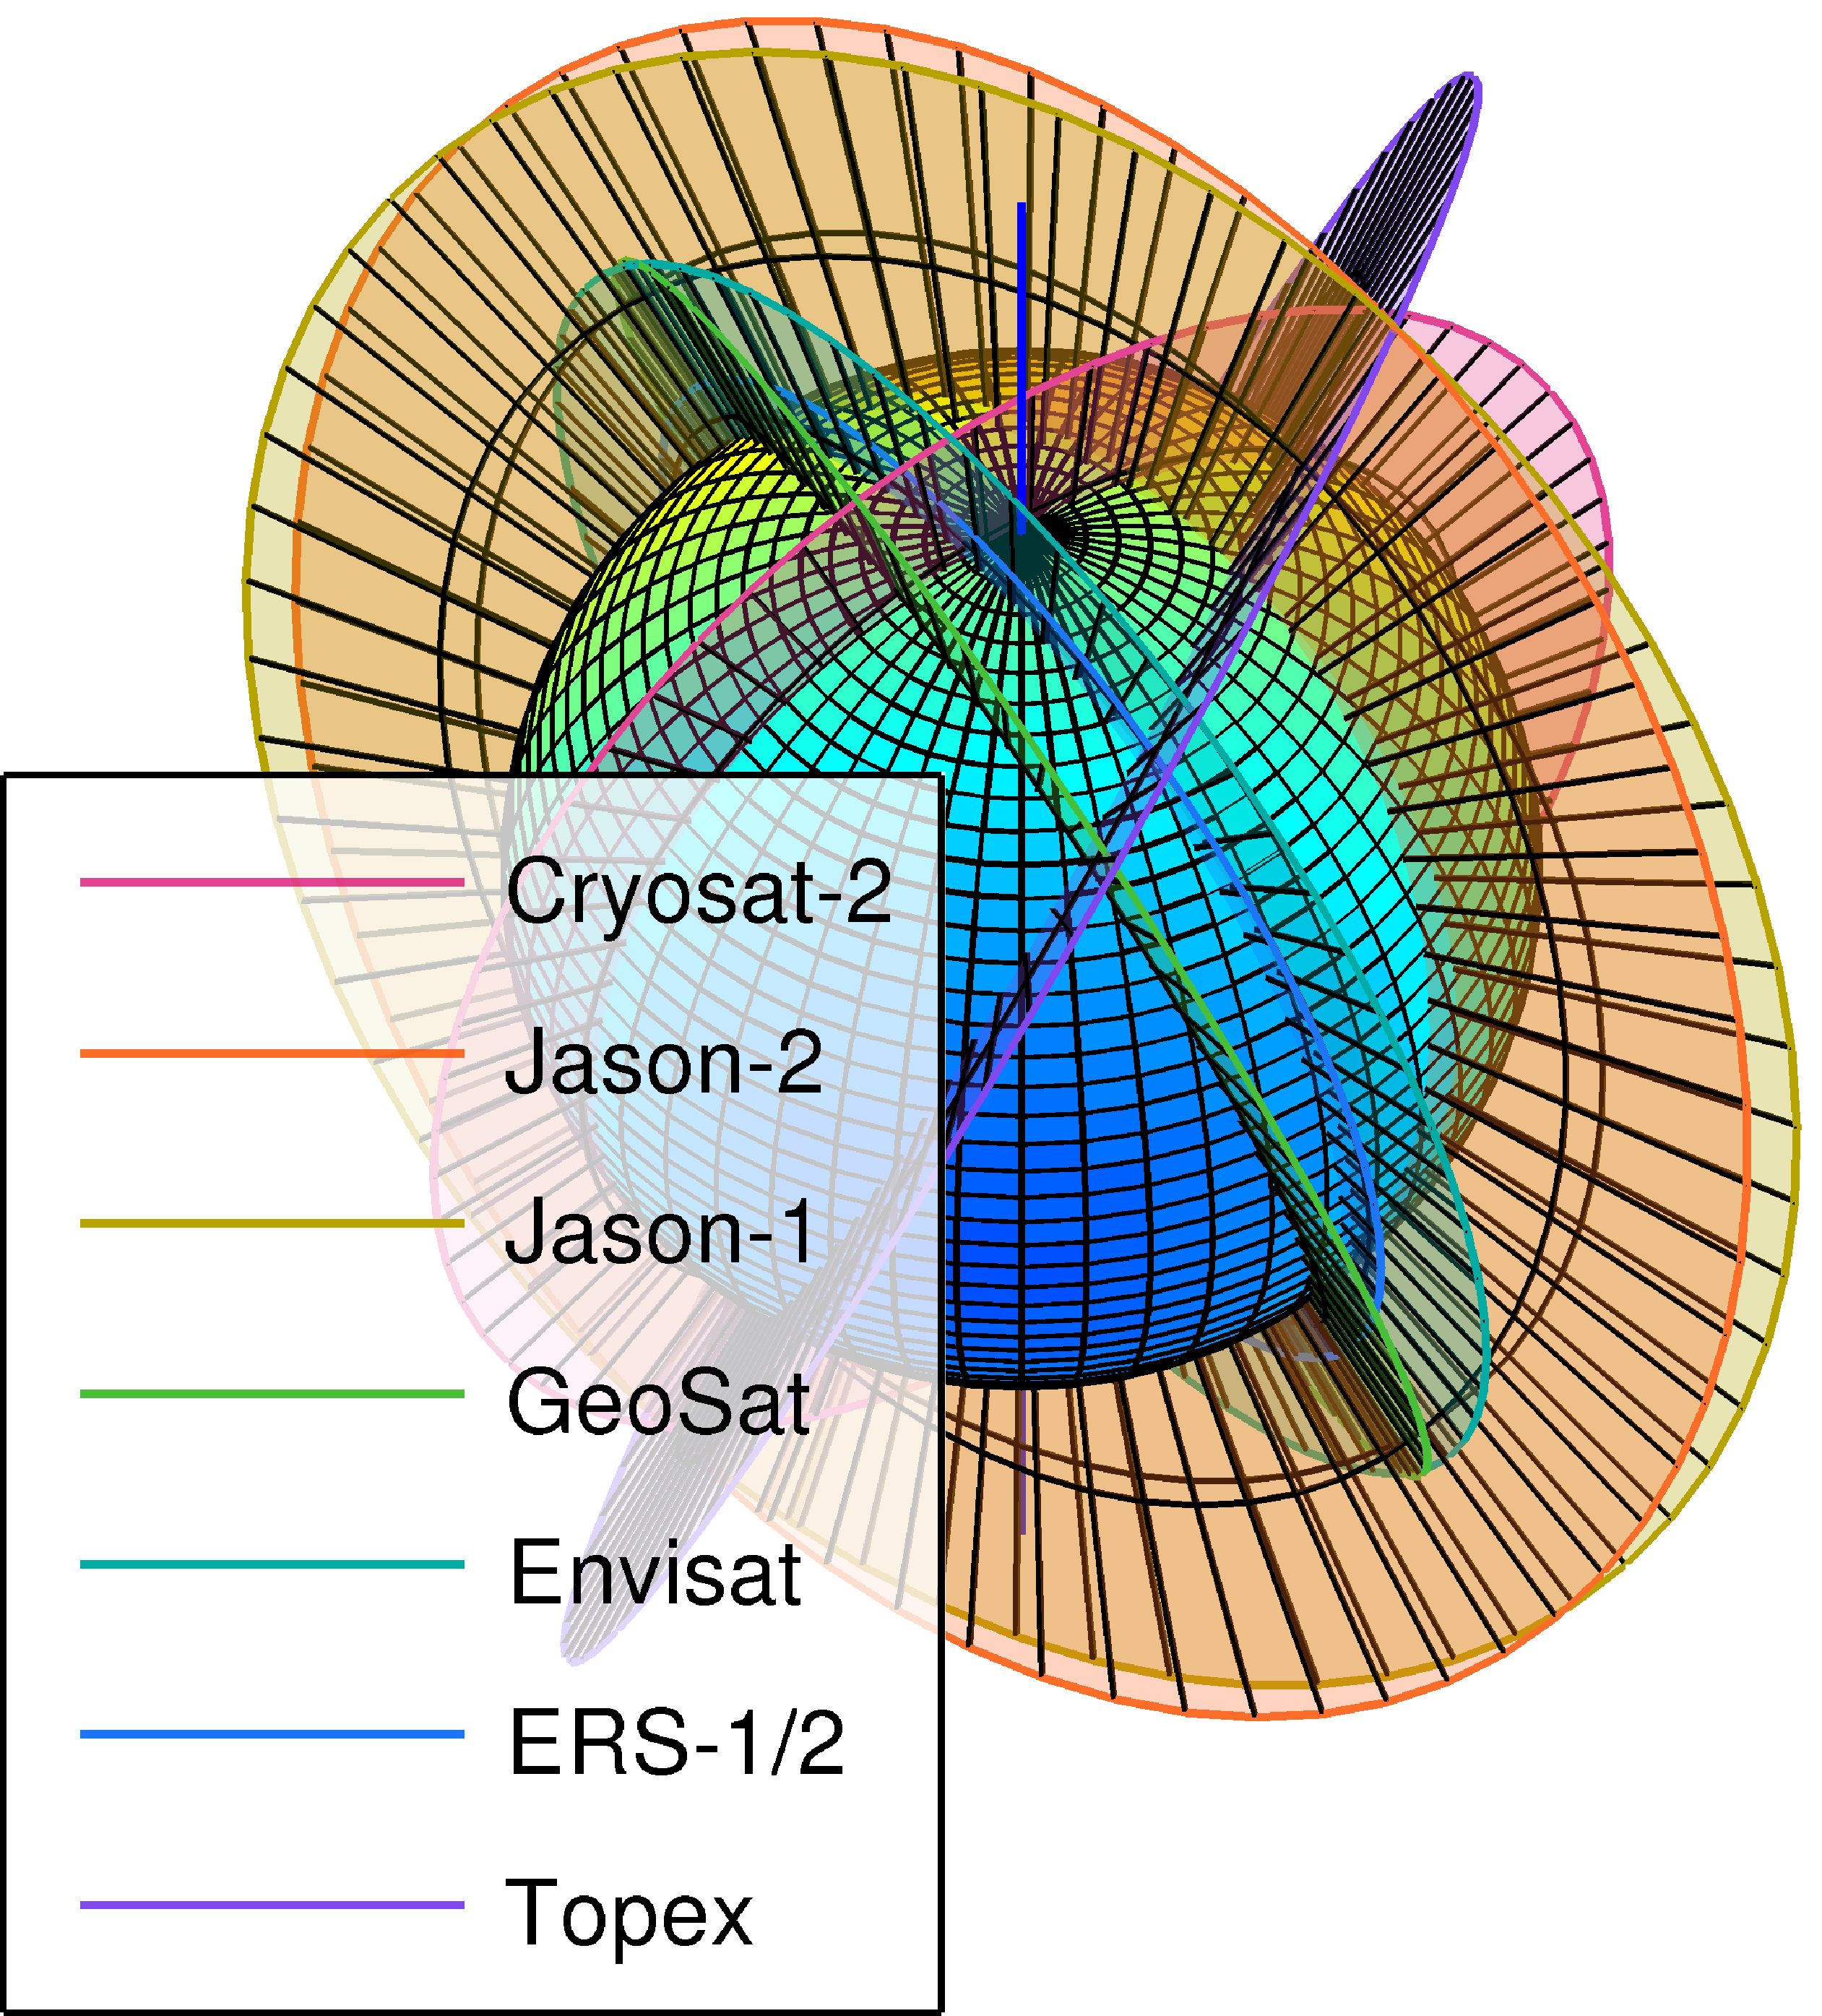
\includegraphics[width=.25\textwidth]{orbits3.pdf}

%\caption{Orbits for Aviso-relevant satellites.}
\end{wrapfigure}

\paragraph{Satellites}The latest Aviso SSH data from satellites features impressive accuracy, constancy and resolutions in both space and time. This is achieved
by collecting all of the data from all of the altimeter-equipped satellites available at any given moment for any given coordinate. This conglomerate of highly
inhomogeneous data is then subjected to state-of-the-art interpolation methods to produce a spatially and temporally coherent product. One satellite alone is
not sufficient to adequately resolve meso-scale variability globally. Take \eg the Topex/Poseidon satellite. It had a ground repeat track orbit of 10 days and
circled the earth in 112 minutes or $\approx 13$ times a day with a swath width of 5 km. Hence it drew $\approx 26$ 5 km-wide stripes onto the globe every day.
This pattern is then repeated after 10 days, which means that at the equator only $10 \times 26 \times 5=1300$km of the $2\pi \times 6371=40000$km get covered,
\ie $3.25\%$. At every $10d$ time step, on average, effectively
$40000/1300-5= 20$km are left blank in-between swaths on the equator. This is why, no matter how fine the resolution within the swath at one moment in time may
be, the spatial resolution is so coarse.



\begin{wrapfigure}[20]{r}{0.6\textwidth}
\vspace{-8mm}
  \begin{center}
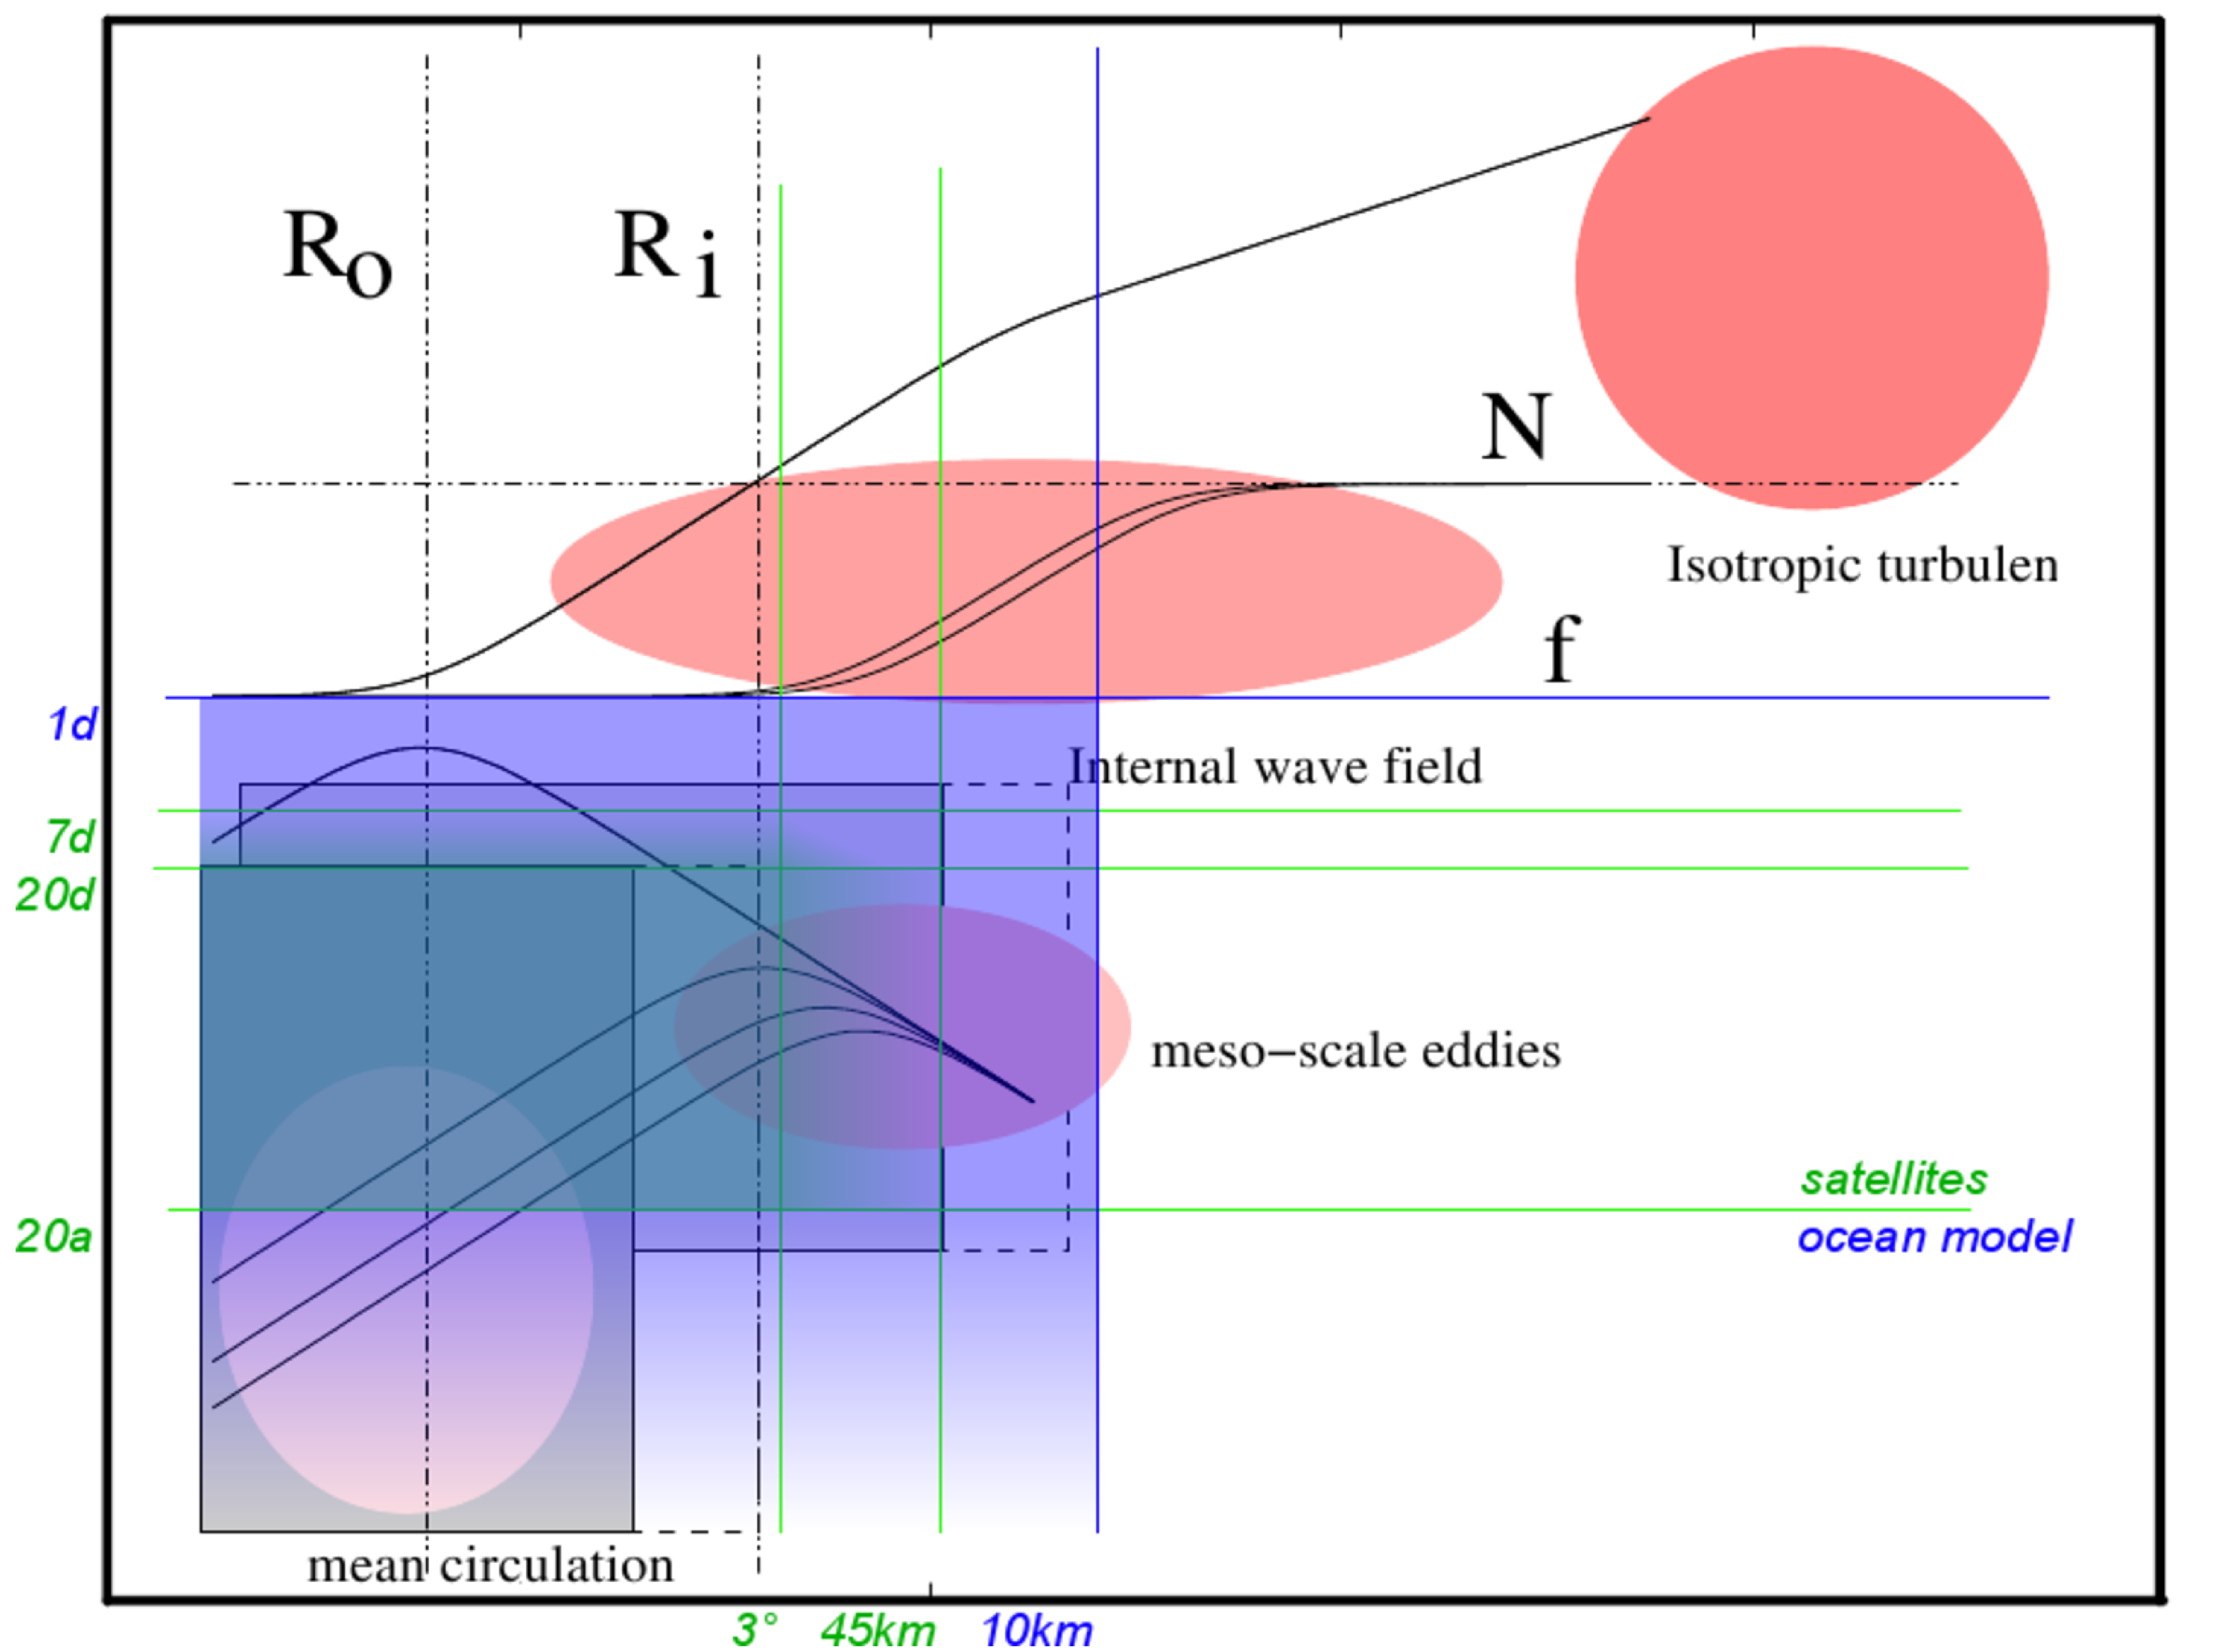
\includegraphics[width=.6\textwidth]{scales.pdf}
 \end{center}
 \vspace{-5mm}
\caption{Resolutions for model vs satellite. Modified version from \cite{olbers2012ocean}.}
\end{wrapfigure}


\begin{figure}[h]
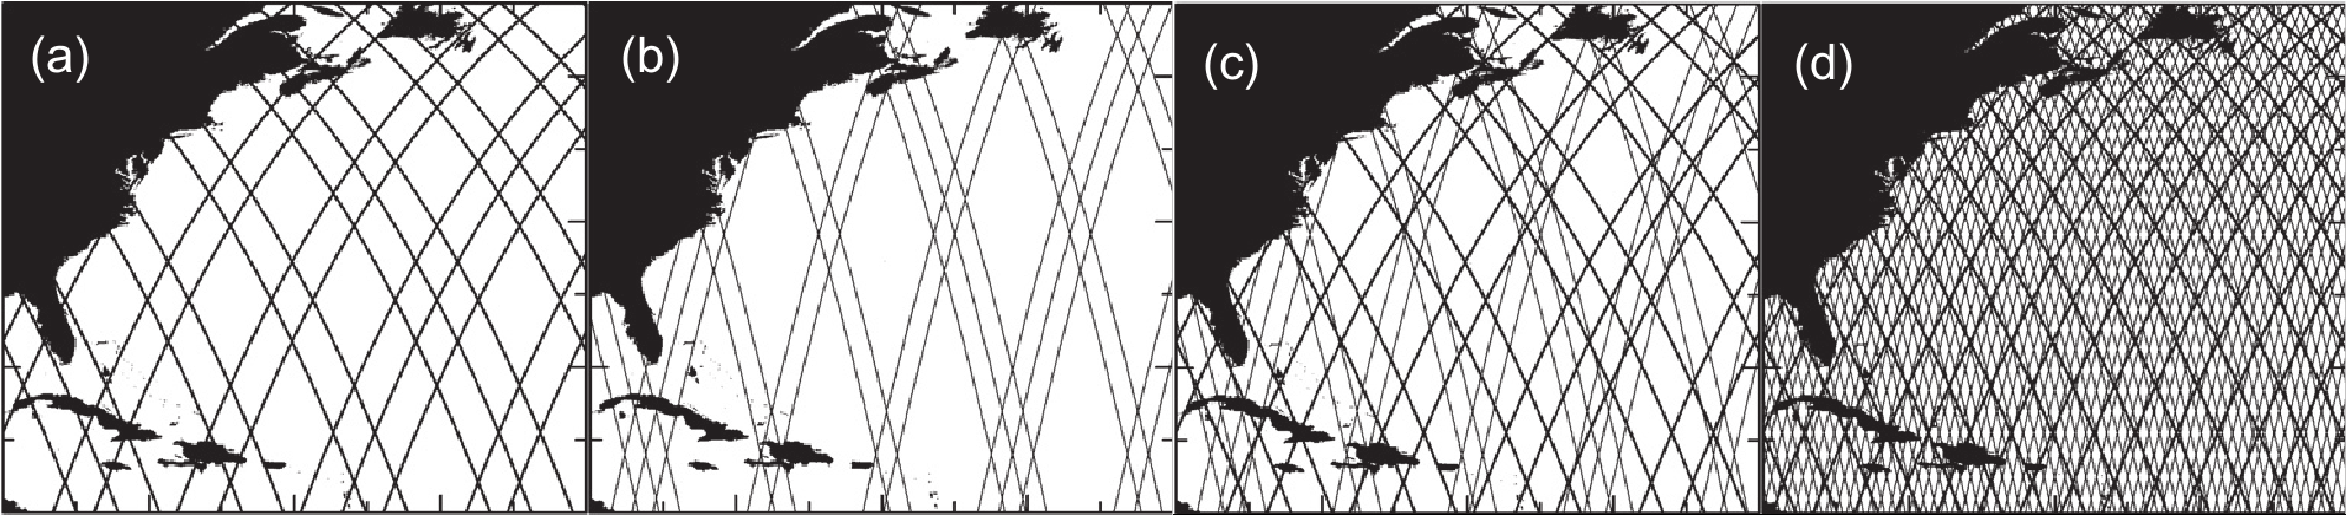
\includegraphics[width=\textwidth]{tracks.pdf}
\caption{{The ground track patterns for the 10-day repeat orbit of T/P and its successors Jason-1 and Jason-2 (thick lines) and the 35-day repeat orbit of ERS-1 and its successors ERS-2 and Envisat (thin lines). (a) The ground tracks of the 10-day orbit during a representative 7-day period; (b) The ground tracks of the 35-day orbit during the same representative 7-day period; (c) The combined ground tracks of the 10-day orbit and the 35-day orbit during the 7-day period; and (d) The combined ground tracks of the 10- day orbit and the 35-day orbit during the full 35 days of the 35-day orbit. (sic)} \cite{Chelton2011}}
\end{figure}


The merged ERS-1/Topex-data as used by \cite{Chelton2011} has a time step of 7 days. Assuming eddy drift speeds of $u_e=\order{-1}$m/s implies a distance traveled per time step of $L_{\delta t}\approx 60km$. \citeauthor{Chelton2011} estimate their effective spatial resolution as $\delta x \approx 40$km. Eddies of smaller scale are not resolved. Tracking a single eddy from one time-step to the next should hence be feasible, especially when $\vec{u}_e$ is approximately known. Problems arise when the sea level is characterized by an abundance of isolated vortices plus maybe even further meso-scale noise of comparable amplitude.
\begin{figure}
\begin{tabularx}{\textwidth}{ |X|X|X| }
  \hline
   & \bf{POP} & \bf{merged T/P - ERS-1 \footnote{the version used by \cite{Chelton2011}}}  \\
  \hline
  dx & $7km-11km$  & $1/3^{\circ}$ ($\approx 40 km$ after filtering)  \\
  \hline
  dt & $1d$  & $7d$  \\
  \hline
  $\log_{10}2$ filter cutoff & n/a  & $2^{\circ} $ by $ 2^{\circ} $  \\
  \hline
  z-levels & 42  & 1  \\
  \hline
  variables & SSH,S,T,u,v,w,tracers  & SSH  \\
  \hline
	pot. interpolation artifacts & n/a  & yes  \\
  \hline
	reality & no  & yes  \\
  \hline
\end{tabularx}
\end{figure}

Ambiguities arise in terms of correctly matching the eddies from the old time-step with those in the new one, potentially causing aliasing effects in the final
statistics. The translational speeds \footnote{$\order{1}$km/day} of eddies are not really the problem here, as they usually drift slow enough to not cover more
than 1 grid node per 7 day time step. The issue are those areas where eddies are born, die and merge. According to \cite{Smith2009} instabilities within the ACC
grow at rates of up to $1/(2 \mathrm{days})$, which means that at a time-step up to 3 eddies have emerged and equally many died for every eddy identified within
such region. The ground-repeat frequency of a satellite can of course not be set arbitrarily. Especially when the satellite is desired to cover as far north and
south as possible, whilst still being subjected to just the right torque from the earth's variable gravitational field to precess at preferably a
sun-synchronous frequency \ie $360^{\circ}/year$. Neither can the
satellite's altitude be chosen arbitrarily. If too low the oblateness of the earth creates too much eccentricity in the orbit that can no longer be
\textit{frozen} \footnote{minimizing undulating signals in altitude by choosing the right initial values.}. Another problem could be potential inhomogeneity in
the merged data in time dimension, since products of old and current missions are lumped together into one product. This is why \cite{Chelton2011} opted against
the finest resolution available and instead went for a product that had the most satellites merged in unison for the longest period of time.

\begin{figure}[h!]
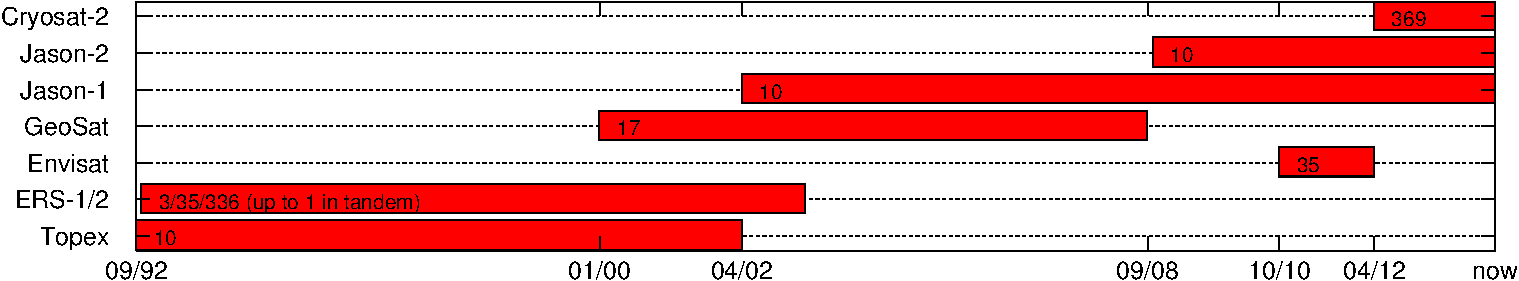
\includegraphics[width=\textwidth]{sats.pdf}
\caption{Length of mission. Numbers are orbit-period in days.}
\end{figure}


%%####################################################################
%%####################################################################

\paragraph{Ocean Model}


\begin{wrapfigure}[20]{r}{0.4\textwidth}
\vspace{-5mm}
  \begin{center}
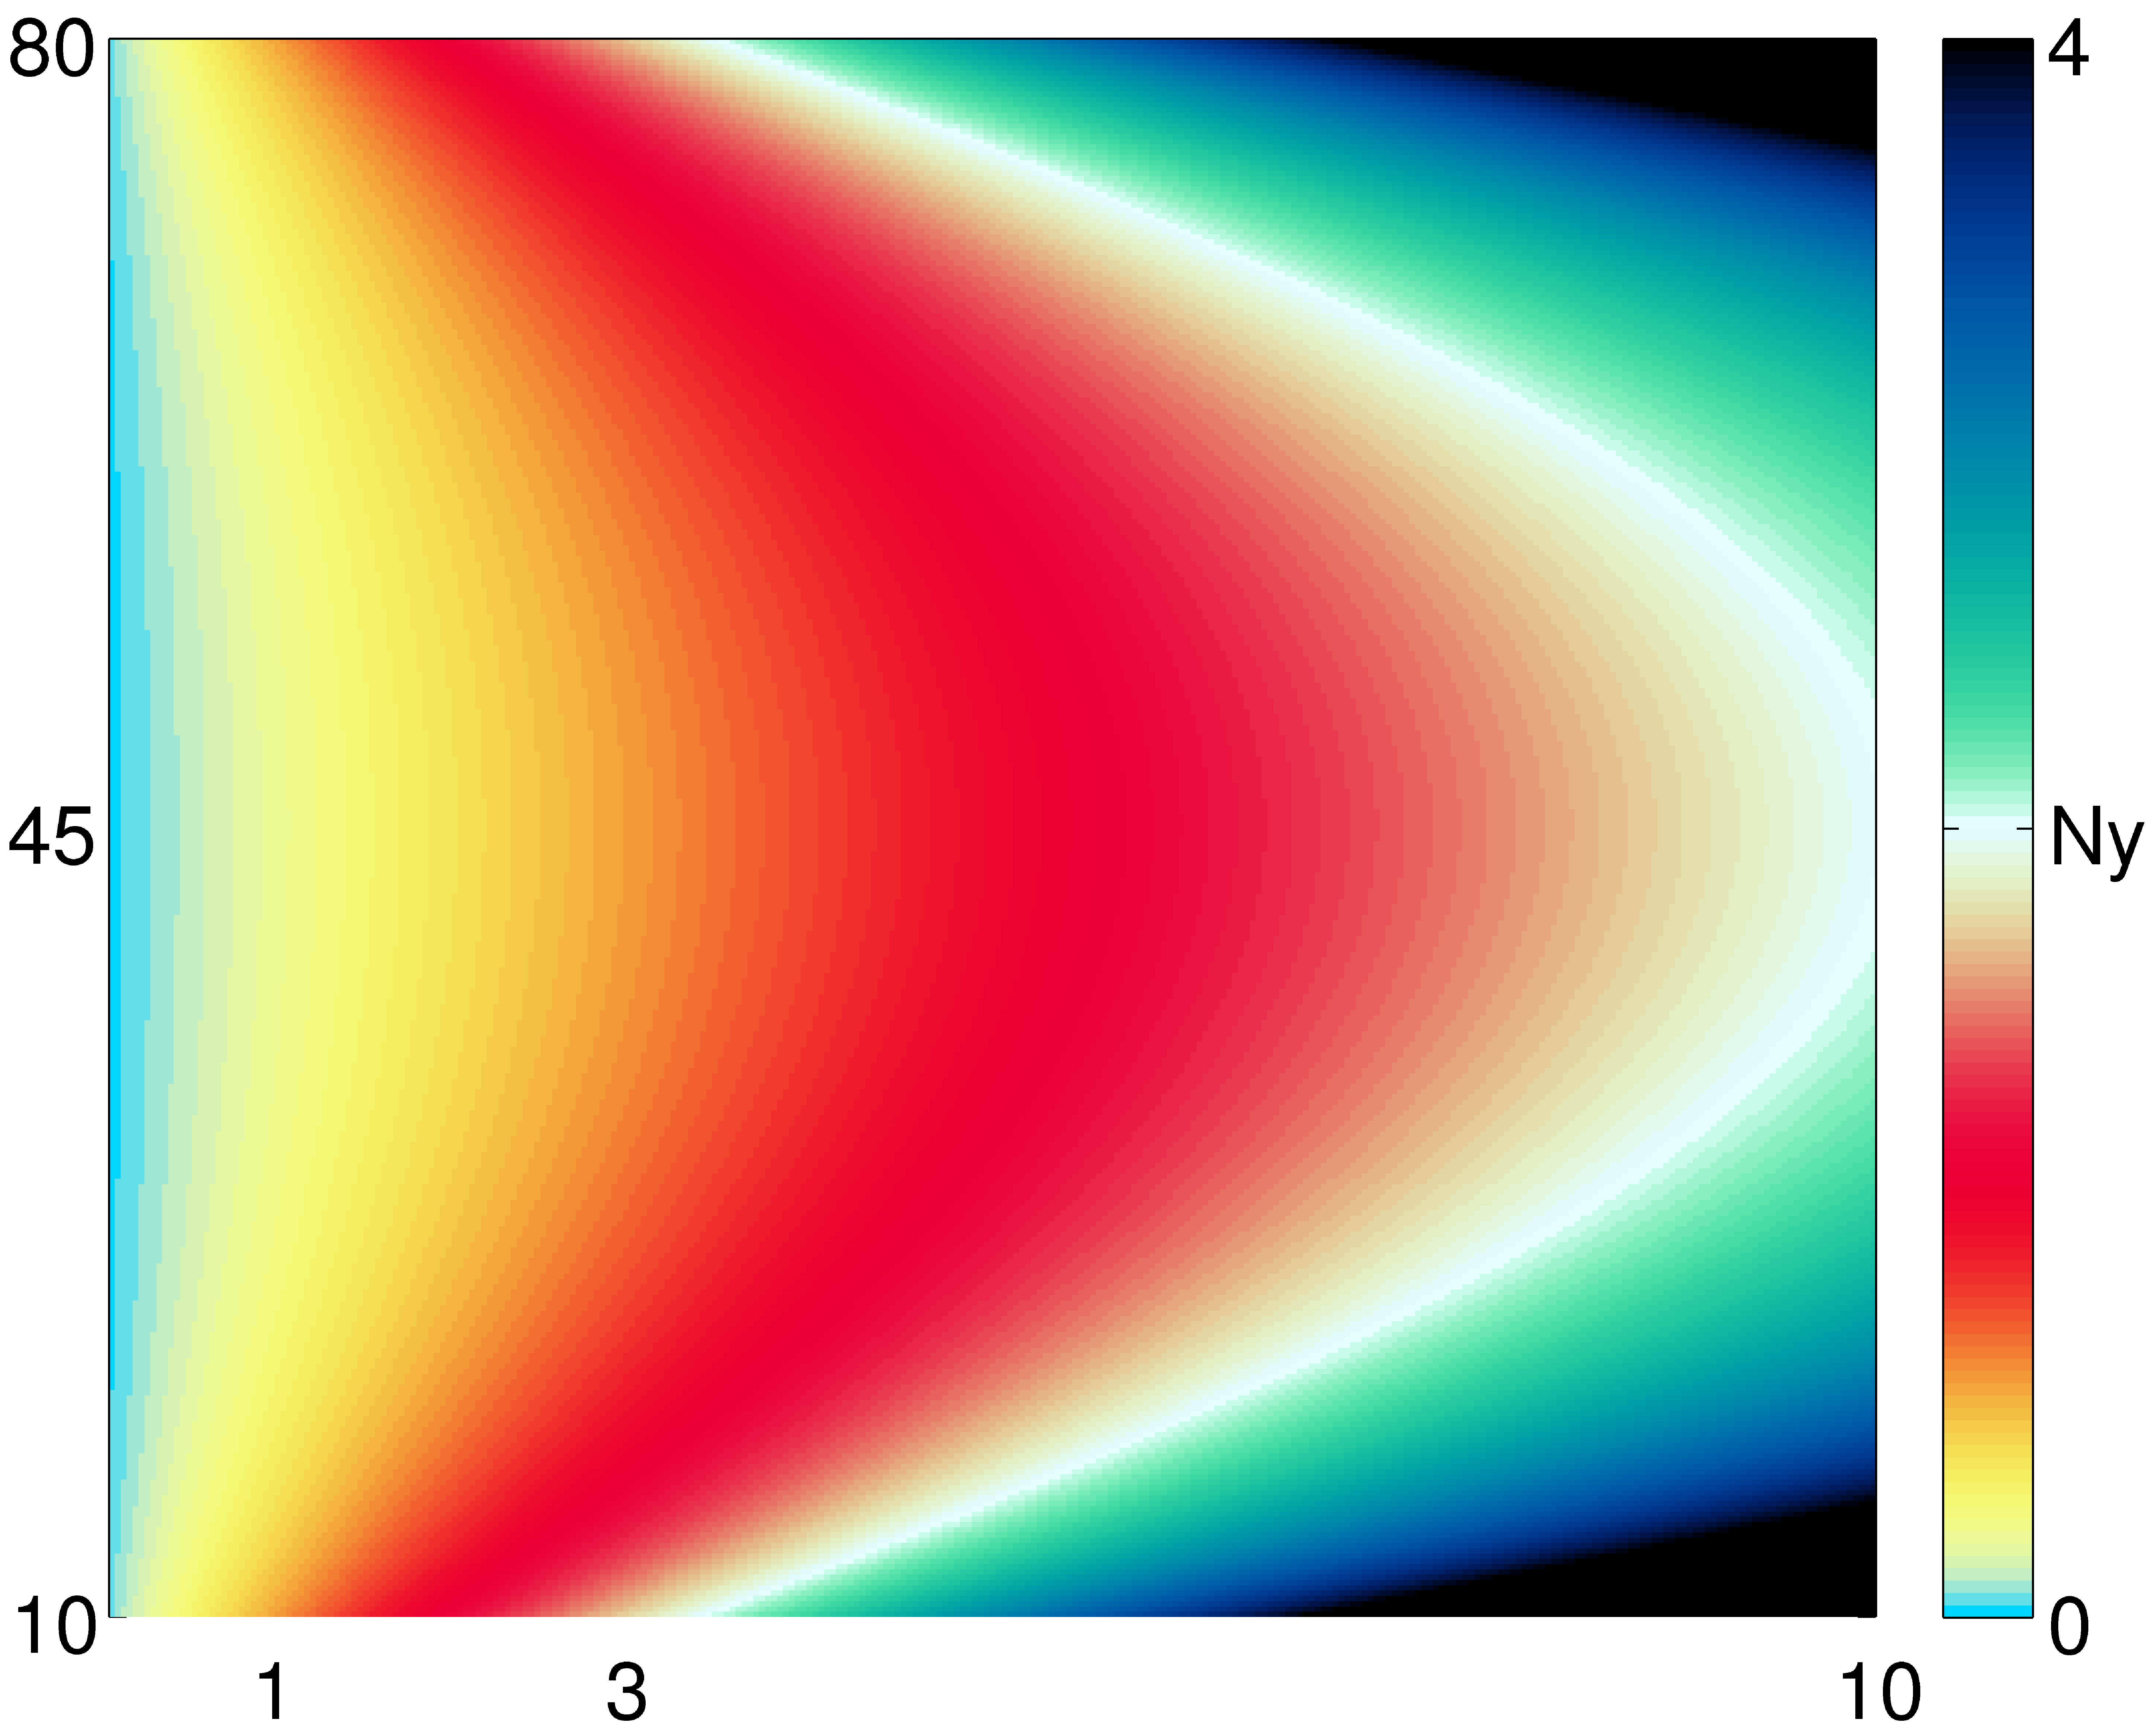
\includegraphics[width=.4\textwidth]{latovermu.pdf}
 \end{center}
  \vspace{-3mm}
\caption{$\xi(\phi,\mu)$. $\mathrm{Ny}\equiv 2$ \ie the Nyquist frequency.}\label{fig:phiovermu}
 %\vspace{-50mm}
\end{wrapfigure}
The advantages of detecting and tracking eddies from model data are obvious.
Say you have $\Bu=1$, so that $L=NH/f$. Let's assume \footnote{corresponds to $L(\phi=30^{\circ})=100$km} $NH=a/10d$, a model resolution of $1^{\circ}/\mu$ and that the eddy diameter was twice the Rossby radius. How many grid notes $\xi$ fit into one eddy as a function of latitude?
%%....................................................................
\begin{align}
	\xi \frac{a}{\mu} \frac{\cos \phi}{2 \pi}
	&=
	\frac{2NH }{f} = \frac{2NH 1d}{4 \pi  \sin(\phi)}\notag\\
	\xi
	&=
	 \frac{ 2\mu }{10  \sin(2\phi)}
\end{align}

See figure~\ref{fig:phiovermu} for the results. In this flat-bottom, constant $\rho_z$, Mercator-gridded model the worst eddy-resolution is interestingly at
mid-latitude. A value of $\xi>2$ is desirable, because it eradicates ambiguities in the tracking procedure, with the result that there is no need to
\textit{forecast} the position $x_e$ of an eddy for the new time step. It suffices to determine the closest eddy from the previous time-step for respective eddy
from the new time step and vice versa. Those 2 eddies that are in agreement are successfully matched, those from the new (old) time step that do not find a
match have just been born (have died). See also section \todoil{ref to section} for the technical stuff.
Another major advantage of the model is that it produces not only SSH data but also all other relevant variables \footnote{See section \ref{sec:goals} for all the
possibilities that arise.}, for not only the surface but for many different depths. The surface velocities inferred from altimetry are the geostrophic
components only, which should suffice to \eg determine the non-linearity and kinetic energy of an eddy for almost all regions, but less so for \eg the western
boundary currents.
The \emph{one} draw-back of using model data is that, in contrast to the satellite data, it does not represent reality.
\footnote{to be continued}


%%--------------------------------------------------------------------
\section{Goals}
%%--------------------------------------------------------------------

\label{sec:goals}



Not all of these will be achieved of course. They will be worked through in the order they appear until the time scope of this thesis is over.
{\bfseries
\begin{enumerate}

\item
Implement an efficient, parallelized, portable, modular algorithm entirely in matlab with focus on straightforwardness, easy maintainability and tweakability.

\item
Mimic the algorithm as described by \cite{Chelton2011} and apply it to the model data.

\item
Repeat all of the analysis done by \cite{Chelton2011} and compare.

\item
Test alternative definition of the \textit{center} of an eddy as the absolute value of the center of volume of the eddy measured from reference height ($z$ of its perimeter).

\item
Test alternative shape-threshold criterion based on isoperimetric coefficient \ie the eddy's sphericity. \footnote{\cite{Chelton2011} guaranteed sphericity by demanding that \textit{The distance between any pair of points within the connected region must be less than a specified maximum.}}.

\item
Compare theoretical phase and group velocities of Rossby waves at wavelength set to determined scale of eddies with eddy velocities.

\item
Compare theoretical wave length of Rossby waves at phase/group speed set to determined drift speed of eddies with eddy scale, similar to \citep{Tulloch2009}.

\item
Compare scales to those derived from linear stability analysis by \eg \cite{Vollmer2013a,eden2012implementing,Smith2009,griesel2013eulerian}.
\end{enumerate}
}

\begin{enumerate}
\setcounter{enumi}{8}
\item
Analyze eddy-genesis and fate. Look at mean values \footnote{either means in time or means in space.} $\Ro$, $\Bu$, $\Rh$, track, scale, as a function of location.

\item
Down-sample the model data, and compare runs for model/satellite at identical
resolution and code.

\item
Go sub-surface and apply the algorithm to at least one other depth than the surface, with the hypothesis that this might help to avoid meso-scale noise in highly turbulent locations.

\item
Use findings from model to improve Aviso tracking.
\item
Filter the SSH-data via Galilean-/LES-decomposition \cite{Adrian2000a} or simply
by a filter created from determined mean shapes of eddies as a function of
location. The motivation is again to successfully track eddies through zones of
strong turbulence.

\item
focus on regions of large Rossby number and regions of strong turbulence (ACC).

\item
Calculate the \emph{effective} Rossby radius as mentioned in \cite{Vollmer2013a} and compare to eddy scales.

\item
Include short lived eddies. \cite{Chelton2011} only analyzed eddies with life times longer than 16 weeks in order to exclude less \textit{robust} eddies for which they did not fully trust their algorithm to be capable of tracking correctly.

\item
Test whether tracers inside eddy stay on isopycnals.

\item
Determine tracks of tracers inside eddy and compare to the eddie's track.


\end{enumerate}

%%--------------------------------------------------------------------

% %####################################################################
 \chapter{The Algorithm}
  This section walks through the algorithm step by step, so as to explain
which
methods are used and how they are implemented.
The idea is that the code from step \mcode{S00..} on can only accept one well
defined structure of data. In earlier versions the approach was to write code
that would adapt to different types of data automatically. All of this extra
adaptivity turned out to visually and structurally clog the code more than it
did offer much of a benefit. The concept was therefor reversed.
\mcode{S00_prep_data} can be altered to produce required output. Yet, there
should be no need to adapt any of the later steps in any way.
All input parameters are to be set in \mcode{INPUT.m} and \mcode{INPUT}\textit{xxx}\mcode{.m}.

%%%%%%%%%%%%%%%%%%%%%%%%%%%%%%%%%%%%%%%%%%%%%%%%%%%%%%%%%%%%%%%%%%%%%%%%%%%%%%%%
%%%%%%%%%%%%%%%%%%%%%%%%%%%%%%%%%%%%%%%%%%%%%%%%%%%%%%%%%%%%%%%%%%%%%%%%%%%%%%%%
\section{Step S00: Prepare Data}
\mcode{function S00_prep_data}	\\
Before the actual eddy detection and tracking is performed,  SSH-, latitude- and longitude-data is extracted from the given data at desired geo-coordinate bounds and saved as structures in the form needed by the next step (S01). This step also builts the file \mcode{window.mat} via \mcode{GetWindow3} which saves geometric information about the input and output data as well as a cross-referencing index-matrix which is used to reshape all \textit{cuts} to the user defined geo-coordinate-geometry. The code can handle geo-coordinate input that crosses the longitudinal seam of
the input data. \Eg say the input data comes in matrices that start and end on
some (not necessarily strictly meridional) line straight across the Pacific and
it is the Pacific only that is to be analyzed for eddies, the output maps are
stitched accordingly. In the zonally continous case \ie the full-longitude case, an \textit{overlap} in x-direction across the \textit{seam}-meridian of the chosen map is included so that contours across the seam can be detected and tracked across it. One effect is that eddies in proximity to the seam can get detected twice at both zonal ends of the maps. The redundant \textit{ghost}-eddies get filtered out in \mcode{S05_track_eddies}. 


%%%%%%%%%%%%%%%%%%%%%%%%%%%%%%%%%%%%%%%%%%%%%%%%%%%%%%%%%%%%%%%%%%%%%%%%%%%%%%%%

 \section{Step S01: Find Contours}
\mcode{function S01_contours}\\
The sole purpose of this step is to apply MATLAB's \mcode{contourc.m} function
to the SSH data. It simply saves one file per time-step with all contour indices
appended into one vector \footnote{see the MATLAB documentation.}. The contour
intervals are determined by the user defined increment and range from the
minimum- to the maximum of given SSH data. \\
The function \mcode{initialise.m}, which is called at the very beginning of
every step, here has the purpose of rechecking the \textit{cuts} for
consistency and correcting the time-steps accordingly (\ie when files are
missing). \mcode{initialise.m} also distributes the files to the threads \ie
parallelization is in time dimension.

%%%%%%%%%%%%%%%%%%%%%%%%%%%%%%%%%%%%%%%%%%%%%%%%%%%%%%%%%%%%%%%%%%%%%%%%%%%%%%%%


\section{Step S01b: Find Mean Rossby Radii and Phase Speeds}
\mcode{function S01b_BruntVaisRossby}\\

This function...
\begin{itemize}
	\item
	\begin{itemize}
		\item
		...calculates the pressure $P(z,\phi)$ in order to...
		\item
		...calculate the Brunt-V\"ais\"al\"a-Frequency according to $N^{2}(S,T,P,\phi)=-\frac{g(\phi)}{P} \frac{\pr \rho(S,T,P)}{\pr z}$
		in order to...	
	\end{itemize}
	\item
	\begin{itemize}
		\item
		...integrate the Rossby-Radius $\Lr=\frac{1}{\pi f}\INT{H}{ }{N}{z}$ and ...
		\item
		apply the long-Rossby-Wave dispersion relation to found $\Lr$ to estimate Rossby-Wave phase-speeds $c=-\frac{\beta}{k^2+(1/L_r)^2} \approx -\beta \Lr^2$
	\end{itemize}
\end{itemize}

The 3-dimensional matrices ($S$ and $T$) are cut zonally into slices which then get distributed to the threads. This allows for matrix operations for all calculations which would otherwise cause memory problems due to the immense sizes of the 3d-data \footnote{\Eg the pop data has dimensions $42 \times 3600 \times 1800 $.}.   


%%%%%%%%%%%%%%%%%%%%%%%%%%%%%%%%%%%%%%%%%%%%%%%%%%%%%%%%%%%%%%%%%%%%%%%%%%%%%%%%
\section{Step S02: Calculate Geostrophic Parameters}
\mcode{function S02_infer_fields}\\ 
This step reads the cut SSH data from \mcode{S00_prep_data} to perform 2 steps:
\begin{enumerate}
\item
Calculate a mean over time of $SSH(y,x)$.
	\item 
\begin{itemize}
	\item  use one of the files' geo-information to determine $\f$, $\dfdy$,
$\g$ and the ratio $\g/\f$.
\item
 calculate geostrophic fields from SSH gradients.
 \item
 calculate deformation fields (vorticity, divergence, stretch and shear) via the
fields supplied by the last step.
\item calculate $\okubo$.
\item
Subtract the mean from step 1 from each $SSH(t)$ to filter out persistent SSH-gradients \eg across the Gulf-Stream.
\end{itemize}


\end{enumerate}
%%%%%%%%%%%%%%%%%%%%%%%%%%%%%%%%%%%%%%%%%%%%%%%%%%%%%%%%%%%%%%%%%%%%%%%%%%%%%%%%

\section{Step S03: Filter Eddies}
\mcode{function S03_filter_eddies}\\ 
Since indices of all possible contour lines at chosen levels are available at
this point, it is now time to subject each and every contour to a
myriad of tests to decide whether it qualifies as the outline of an eddy as
defined by the user input threshold parameters.
\subsection*{Reshape for Filtering and Correct out of Bounds Values}
\mcode{function eddies2struct}\\
\mcode{function CleanEddies}\\
In the first step the potential eddies are transformed to a more sensible
format, that is, a structure \mcode{Eddies(EddyCount)} where \mcode{EddyCount}
is the number of all contours. The struct has fields for level, number of
vertices, exact \ie interpolated coordinates and rounded integer coordinates.\\
The interpolation of \mcode{contourc.m} sometimes creates indices that are
either smaller than $0.5$ or larger than $N+0.5$ \footnote{where $N$ is the
domain size} for contours that lie along a boundary. After rounding, this
seldomly leads to indices of either $0$ or $N+1$. These values get set to $1$
and $N$ respectively in this step.
\subsection*{Descent/Ascend Water Column and Apply Checks}
The concept of this step is a direct adaption of the algorithm described
by \cite{Chelton2011}. It is split into two steps, one for anti-cyclones and one
for cyclones. Consider \eg the anti-cyclone situation. Since all
geostrophic anti-cyclones are regions of relative high pressure, all
anti-cyclones \footnote{henceforth abbreviated AC} effect an elevated \SSH \ie
a \textit{hill}. The algorithm ascends the full range of SSH levels where
contours were found. Consider an approximately Gaussian shaped AC that has a
peak SSH of say 5 increments larger than the average surrounding waters. 
As the algorithm approaches the sea surface from below, it will eventually run
into contours that are closed onto themselves and that encompass the AC. At
first these contours might be very large and encompass not only one but several
ACs and likely also cyclones, but as the algorithm continues upwards found
contour will get increasingly circular, describing some outer \textit{edge} of
the AC. Once the contour and its interior pass all of the tests the algorithm
will decide that an AC was found and write it and all its parameters to disk.
The AC's region \ie the interior of the contour will be flagged from here on.
Hence any inner contour further up the water column will not pass the tests.
Once all AC's are found for a given time-step, the SSH flags get reset and the
entire procedure is repeated only this time \textit{descending} the SSH-range to
find cyclones. The tests for cyclones and anti-cyclones are identical except for
a factor $-1$ where applicable. In the following the most important steps of the
analysis are
outlined. 
\subsubsection{NaN-Check Contour}
\mcode{function CR_RimNan}\\
The first and most efficient test is to check whether indices of the
contour are already flagged. Contours within an already found eddy get thereby
rejected immediately.
%\subsubsection{Closed Ring}
%\mcode{function CR_ClosedRing}\\
%Contours that do not close onto themselves are obviously not eligible for
%further testing.
\subsubsection{Sub-Window}
\mcode{function get_window_limits}\\
\mcode{function EddyCut_init}\\
For further analysis a sub-domain around the eddy is cut out of the SSH data.
These functions determine the indices of that window and subtract the
resultant offset for the contour indices. 
\subsubsection{Logical Mask of Eddy Interiour}
\mcode{function EddyCut_mask}\\
Basically this function creates a
\href{http://en.wikipedia.org/wiki/Flood_fill}{flood-fill} logical mask of the
eddy-interior. This is by far the most calculation intensive part of the whole
filtering procedure. A lot more time was wasted on attempting to solve this
problem more efficiently than time could have been saved would said attempts
have
been successful. The current solution is basically just MATLAB's
\mcode{imfill.m}, which was also used in the very first version of 09/2013.
EDIT: \mcode{imfill.m} was replaced by using \mcode{inpoly.m} to determine which indices lie within the contour-polygon. This method seems to be more exact at determining whether the inside-part of one grid cell (with respect to the smooth, spline-interpolated contour) is larger than the outside part or not.  
%\subsubsection{Islands}
%\mcode{function CR_Nan}\\
%No flags within the eddy are allowed. This check also avoids contours around
%islands as all land is flagged \textit{a priori}.
\subsubsection{Sense}
\mcode{function CR_sense}\\
\textbf{All} of the interior SSH values must lie either above or below current
contour level, depending on whether anti-cyclones or cyclones are sought.
\subsubsection{Area} \label{filter:area}

sdhsrthert TODO
 area.pixels = (z.fields.dx.*z.fields.dy).*(z.mask.inside + z.mask.rim_only/2);  % include 'half of rim'
    area.total = sum(area.pixels(:));
    area.meanPerSquare = mean(z.fields.dx(z.mask.filled).*z.fields.dy(z.mask.filled));
    area.intrp = area.meanPerSquare*polyarea(z.coor.exact.x,z.coor.exact.y);
    area.RadiusOverRossbyL = sqrt(area.intrp/pi)/rossbyL;

\mcode{function EddyCircumference}\\
Area described by the contour. This is needed for \ref{filter:shape}. This is
not however related to the actual eddy scale determined in
\ref{filter:dynscale}.
\subsubsection{Cirumference}
\mcode{function EddyCircumference}\\
Line-length (sum of Euclidean norm of all nodes) of the contour.
\newpage
\subsubsection{Shape}\label{filter:shape}
\mcode{function CR_Shape}\\
\begin{wrapfigure}{r}{0.4\textwidth}
	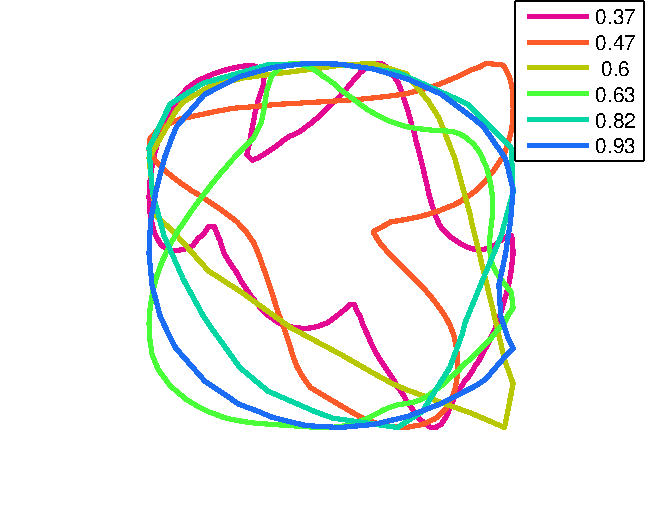
\includegraphics[width=0.45\textwidth]{isoper}
	\caption{Different values of the isoperimetric quotient.}
	\label{fig:isoper}
\end{wrapfigure}

This is the crucial part of deciding whether the object is \textit{round
enough}. A perfect vortex with $\dpr{u}{y}=-\dpr{v}{x}$ is necessarily a
circle. The problem is that eddies get formed, die, merge, run into obstacles,
get asymmetrically advected etc. To successfully track them it is therefor
necessary to allow less circle-like shapes whilst still avoiding to \eg count 2
semi merged eddies as one. 
This is achieved by calculating the \hyperref[def:IQ]{isoperimetric quotient},
defined as the ratio of a ring's area to the area of a circle with equal
circumference. \cite{Chelton2011} use a similar method. They
require:\\ \textit{The distance between any pair of points within the connected
region must be less than a specified maximum} \citep{Chelton2011}.\\
While this method clearly avoids overly elongated shapes it allows for stronger
deformation within its distance bounds. \todo{compare both, show pictures}
\subsubsection{Amplitude} \label{filter:amp}
\mcode{function CR_AmpPeak}\\
This function determines the amplitude \ie the maximum of the absolute
difference between SSH and current contour level and the position thereof as
well as the amplitude relative to the mean SSH value of the eddy interior as
done by \cite{Chelton2011}. The
amplitude is then tested against the user-given threshold. The function also
creates a matrix with current contour level shifted to zero and all values
outside of the eddy set to zero as well. 
\subsubsection{Profiles}
\mcode{function EddyProfiles}\\
This step saves the meridional and zonal profiles of SSH, U and V. 
\begin{wrapfigure}{r}{0.4\textwidth}
	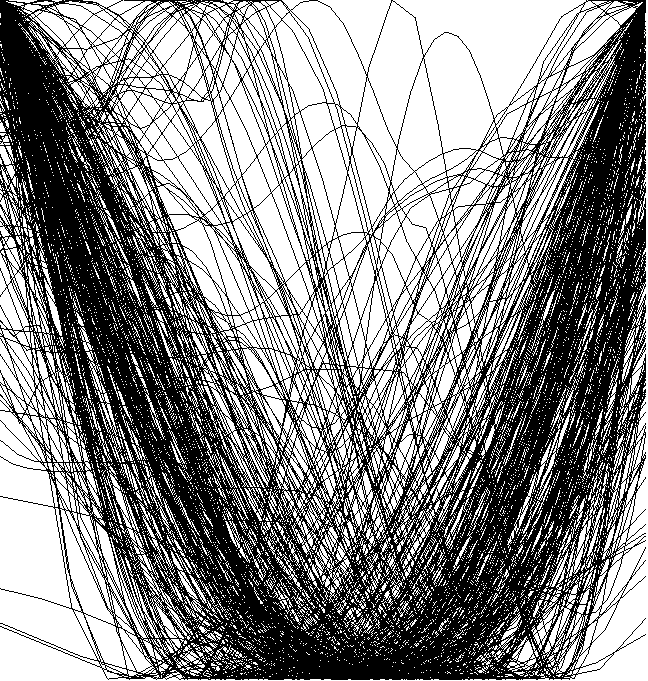
\includegraphics[width=0.4\textwidth]{profiles}
	\caption{Zonal $x$- and $z$-normalized cyclone-profiles.}
	\label{fig:profiles}
\end{wrapfigure}

\subsubsection{\textit{Dynamic} Scale} \label{filter:dynscale}
\mcode{function EddyRadiusFromUV}\\
The contour line that is being used to detect the eddy is not
necessarily a good measure of the eddy's \textit{scale} \ie it doesn't
necessarily represent the eddy's outline very well. This becomes very 
obvious when the area, as inferred by \ref{filter:area}, is plotted over time
for an already successfully tracked eddy. The result is not a smooth curve at
all. This is so because at different time steps the eddy usually gets detected
at different contour levels. Since its surrounding continuously changes and
since the eddy complies with the testing-criteria the better the closer the
algorithm gets to the eddy's peak value, the determined area of the contour
jumps considerably between time steps. This is especially so for large flat
eddies with amplitudes on the order of $1cm$. If the contour increment is on
that scale as well, the difference in contour-area between two time steps 
easily surpasses $100\%$ and more. 
Since there is no definition for the \textit{edge} of an eddy, it is here
defined as the ellipse resulting from the meridional and zonal diameters that
are the distances between first minimum and maximum orbital velocity, away from
the eddy's peak in positive and negative y and x directions respectively. 
In the case of a meandering jet with a maximum flow speed at its center, that
is shedding off an eddy, this scale corresponds to half the distance between
two opposing center-points of the meander. It is also the distance at which a
change in vorticity polarity occurs and is thus assumed to be the most plausible
\textit{dividing line} between vortices. 
\todo{theres probably a better way via okubo weiss!}
In practice the velocity-gradient profiles need to be smoothed to successfully
determine their first adequate zero-crossing. Once the zero crossings in all
4 directions are found, their mean is taken as the eddy's scale. Note that this
is again similar to what \cite{Chelton2011} did. 
\subsubsection{\textit{Dynamic} Amplitude}
\mcode{function EddyAmp2Ellipse}\\
As mentioned above, the contour that helps to detect the eddy is not
representative of its extent. This is also true for the $z$-direction, for the
same reasons. This function therefor takes an SSH-mean at indices of the ellipse
created by the determined zonal and meridional \textit{dynamical} diameters,
and uses this as the basal value to determine a \textit{dynamic} amplitude.
\subsubsection{Center of Volume}
\mcode{function EddyArea2Ellipse}\\
\mcode{function CenterOfVolume}\\
Instead of using the geo-position of the eddy's peak in the tracking procedure,
it was decided to instead use the center of the volume created by the basal
shifted matrix from \ref{filter:amp} \ie \textit{the center of volume of the
dome
(resp. valley) created by capping off the eddy at the contour level}.
This method was chosen because from looking at animations of the tracking
procedure
it became apparent that, still using peaks as reference points, the eddy
sometimes jumped considerably from one time step to the next if two local maxima
existed within the eddy. \Eg in one time-step local maximum $A$ might be just a
little bit larger than local maximum $B$ and one time-step later a slight shift
of mass pushes local maximum $B$ in pole position, creating a substantial jump
in the eddy-identifying geo-position hence complicating the tracking procedure. 
\section{Step S04: Track Eddies}
\mcode{function function S04_track_eddies}\\
Due to the the relatively fine temporal resolution (daily) of the model data,
the tracking procedure turns out to be much simpler than the one described by
\cite{Chelton2007}. There is really no need to project the new position of an
eddy, as it generally does not travel further than its own scale in one day.
This means that one eddy can be unambigiously tracked from one time step to the
next as long both time-steps agree on which eddy from the other
time-step is located the least distance away.
The algorithm therefor simply builds an arc-length-distance matrix
between all old and all new eddies and then determines the minima of that
matrix in both directions \ie one array for the new with respect to the old,
and one for the old with respect to the new set. This leads to the following
possible situations:
\begin{itemize}
	\item 
	Old and new agree on a pair. \Ie old eddy $O_a$ has a closest neighbour in
the new set $N_a$ and $N_a$ agrees that $O_a$ is the closest eddy from the old
set. Hence the eddy is tracked.  $N_a$ is $O_a$ at a later time.
\item
$N_a$ claims $O_a$ to be the closest, but $N_b$ makes the same claim. \Ie two
eddies from the new set claim one eddy from the old set to be the closest. 
In this situation the closer one is decided to be the old one at a later
time-step and the other one must be a newly formed eddy.
\item 
At this point all new eddies are either allocated to their respective old
eddies or assumed to be \textit{newly born}. The only eddies that have not been
taken care of are those from the old set, that \textit{lost} ambigious claims to
another old eddy, that was closer to the same claimed new eddy. \Ie there is no
respective new eddy available which must mean that the eddy just \textit{died}.
In this case the entire track with all the information for each time step is
saved as long as the track-length meets the threshold criterium. If it doesn't,
the track is deleted. 
\end{itemize}

\section{Step S05: Cross Reference Old to New Indices}
\mcode{function function S05_init_output_maps}\\
The main purpose of this step is to allocate all grid nodes of the input data
to the correct node of the output map. Since the output map is usually much
coarser than the input data there is no need for interpolation.  

\section{Step S06: Make Maps of Mean Parameters}
\mcode{function function S06_analyze_tracks}\\
 

\section{Example}
To show a hands-on example an exemplary run for part of the North Atlantic is
demonstrated in the following. 
\subsection{Map Parameters} \label{codeEx:map_params}
The geo-coordinates for the map window are to be set in \mcode{map_vars.m}.
In this case a small region in the eddy-rich North Atlnatic from $-90^\circ$
west till $-40^\circ$ west and from $20^\circ$ north till $60^\circ$ north is
chosen. This script has an effect only on the very first step (\mcode{S_00..}).
\begin{lstlisting}
function MAP=map_vars
	%% user input
	MAP.geo.west=-90;
	MAP.geo.east=-40;
	MAP.geo.south=20;
	MAP.geo.north=60;
	MAP.time.delta_t = 1; % [days]
	MAP.SSH_unitFactor = 100; % eg 100 if SSH data in cm, 1/10 if in deka m etc..
	MAP.pattern.in='SSH_GLB_t.t0.1_42l_CORE.yyyymmdd.nc';
end
\end{lstlisting}
\todo{show map}
\subsection{Other Parameters}
All other parameters are to be set in \mcode{input_vars.m}. 
\begin{itemize}
	\item 
	The maximum number of \textit{local workers} (threads) is at default settings
usually limited to 12 by Matlab. Hence 
 \begin{lstlisting}
 	U.threads.num=12;
 \end{lstlisting}
 \item 
 The data available at this point in time spans from 1994/04/02 till 2006/12/31.
Hence
 \begin{lstlisting}
 	U.time.from.str='19940402';
  	U.time.till.str='20061231';
 \end{lstlisting}
\item 
Data is available per day. Therefor \mcode{U.time.delta_t=1; } is set
to 1. This could also be changed to another value, if the user wished to skip
time-steps.
	\item \label{codeEx:data}
	The path \mcode{U.path.root='../dataXMPL/';} can be set arbitrarily. If it
does not yet exist, it will be created. It is suggested to not reuse a path,
as this could lead to inconsitencies in the data.
\item
\todo{ \mcode{	U.path.TempSalt.name='TempSalt/';}}
\item
\mcode{U.path.raw.name='/scratch/uni/ifmto/u241194/DAILY/EULERIAN/SSH/';}\\
This is where the SSH data is stored.
\item
\begin{lstlisting}
	U.contour.step=0.01; % [SI]
	U.thresh.radius=5e3; % [SI]
	U.thresh.amp=0.02; % [SI]
	U.thresh.shape.iq=0.5; % isoperimetric quotient
	U.thresh.shape.chelt=0.5; % (diameter of circle with equal area)/(maximum
distance between nodes) (if ~switch.IQ) 
	U.thresh.corners=6; % min number of data points for the perimeter of an eddy
	U.thresh.dist=1*24*60^2; % max distance travelled per day
	U.thresh.life=20; % min num of living days for saving
\end{lstlisting}
In this segment the following values are set (all in SI-units, except for
time dimension).:
	\begin{itemize}
		\item 
		The contour intervall with which to look for SSH-contours from maximum to
	minimum SSH-value.
	\item
	The minimum radius threshold for an eddy.
	\item
	The minimum amplitude threshold.
	\item
	Either the minimum $\IQ$ value or the minimum ratio of the diameter of a
circle	 with equal area over the maximum distance between nodes, depending on
which	 method is chosen (see ). 
	\item
	The minimum number of grid nodes making up the contour.
	\item
	The maximum distance-travelled-per-timestep threshold.
	\item
	The minium track-length (in time) threshold for a track to be saved.
	\end{itemize}
\item

\begin{lstlisting}
	U.dim.X=40*1+1;
	U.dim.Y=40*1+1;
	U.dim.west=-90;
	U.dim.east=-50;
	U.dim.south=20;
	U.dim.north=60;
	U.dim.NumOfDecimals=1;
\end{lstlisting}
These paramters describe the output maps, that will be created in the very end
(\eg maps of mean values). Ideally they are set to the same limits as
those set in \ref{codeEx:map_params}. \mcode{U.dim.X}/\mcode{U.dim.Y} dictate
the size of the output maps. They can be set arbitrarilly, but the format \eg
$(east-west)*n +1; \;\; n \in \mathrm{N}$ is suggested to avoid long decimals in
the coordinate matrices.
\item
\begin{lstlisting}
	U.switchs.RossbyStuff=false;
	U.switchs.IQ=true;	
\end{lstlisting}
Choose whether step \mcode{S01b_BruntVaisRossby} is to be run (needs adequate
salt and temperature files \todo{explain}) and the type of shape-testing (
\mcode{U.switchs.IQ=true}) for $\IQ$-method.
\item
The rest are less important technical things that are only relevant if the code
itself is modulated (\eg if modules are added).
\end{itemize}

%%%%%%%%%%%%%%%%%%%%%%%%%%%%%%%%%%%%%%%%%%%%%%%%%%%%%%%%%%%%%%%%%%%%%%%%%%%%%%%%
\subsection{Running the Code}
The seperate steps can be run all at once via \mcode{Sall.m} or one by one, as
long as they are started consecutively in the order indicated by their name
( \mcode{S00..}, then \mcode{S01..} \etc). \mcode{S01b} is not necessary
though. Each step saves its own files which are then read by the next step.
All output data is saved in the user given root-path from \ref{codeEx:data}.
This concept uses quite a lot of disk space and is also quite substantially
slowed by all the reading and writing procedures. The benefits, on the other
hand, are that debugging becomes much easier. If the code fails at some step,
at least all the calculations up to that step are dealt with and do not need to
be re-run. The concept also makes it easy to extend the code by further
add-ons.

\todo{plots to follow...}



\href{https://github.com/PremKolar/MT4}{see github for progress}

















 % Define block styles
\tikzstyle{input} =  = [diamond, draw, fill=green!20,
    text width=2.5em, text badly centered, node distance=3.5cm, inner sep=0pt]
\tikzstyle{block} = [rectangle, draw, fill=blue!20, 
    text width=4.5em, text centered, rounded corners, node distance=1.7cm,
minimum height=1.5em]
\tikzstyle{line} = [draw, very thick, color=black!50, -latex']
\tikzstyle{data} = [draw, ellipse,fill=red!20,
    text width=3.5em, node distance=2.7cm,
    minimum height=2.5em]
        
    
\begin{scriptsize}
\begin{figure}
	\centering
	
\begin{tikzpicture}[node distance = 1.7cm, auto]    
    \node [input] (input_vars) {user input};
    \node [input, right of=input_vars] (map_vars) {map input};
    
    \node [block, below of=map_vars] (S00) {S00 - prepare data};
    \node [block, below of=S00] (S01) {S01 - get contours};
    \node [block, below of=S01] (S02) {S02 - infer fields};
    \node [block, below of=S02] (S03) {S03 - filter contours};
    \node [block, below of=S03] (S04) {S04 - track eddies};
    \node [block, below of=S04] (S05) {S05 - initialize output maps};
    \node [block, below of=S05] (S06) {S06 - analyze tracks};
    \node [block, below of=S06] (S07) {S07 - plotting stuff};
    
    \node [data, left of=S00] (Draw) {raw SSH data};
    \node [data, right of=S00] (Dcuts) {formated SSH data};
    \node [data, left of=S02] (Dconts) {daily contour data};
    \node [data, right of=S03] (Deddies) {filtered contours};
    \node [data, right of=S05] (Dtracks) {tracks};
  %  \node [data, right of=Deddies] (DD) {Sall output};
    \node [data, right of=S06] (plotready) {formated for plot};
    \node [data, right of=S07] (plots) {plots};
    \node [data, left of=S06] (indx) {referenced indices};
    
    \path [line,dashed] (input_vars) -- (S00);
    \path [line,dashed] (input_vars) |- (S03);
    \path [line,dashed] (input_vars) |- (S04);
    \path [line,dashed] (input_vars) |- (S05);
    \path [line,dashed] (input_vars) |- (S07);
    \path [line,dashed] (map_vars) -- (S00);
    \path [line] (Dcuts) -- (S05);    
    
    \path [line] (Draw) -- (S00);
    \path [line] (S00) -- (Dcuts);
    \path [line] (Dcuts) -- (S01);
    \path [line] (S01) -- (Dconts);
    \path [line] (S02) -- (Dcuts);
    \path [line] (Dcuts) -- (S02);
    \path [line] (Dconts) -- (S03);
    \path [line] (S03) -- (Deddies);
    \path [line] (Dcuts) -- (S03);
    \path [line] (Deddies) -- (S04);
    \path [line] (S04) -- (Dtracks);
    \path [line] (Dtracks) -- (S06);
    \path [line] (S06) -- (plotready);
    \path [line]  (plotready) -- (S07);
    \path [line]   (S07) -- (plots) ;
    \path [line]   (S05) -- (indx) ;
    \path [line]   (indx) -- (S07) ;    
\end{tikzpicture}

	\caption{Basic code structure. Input is green, code is blue and data is red.}
	\label{fig:codeflow}
\end{figure}

\end{scriptsize}
     

% \chapter{Results}
% \todo[inline]{results...}
% \chapter{Discussion}
% \todo[inline]{discussion...}
% 
% %
% % ####################################################################
% % ####################################################################
% %
% \renewcommand{\thechapter}{\Alph{chapter}}
% \setlength{\belowdisplayskip}{2pt} \setlength{\belowdisplayshortskip}{1pt}
% \setlength{\abovedisplayskip}{2pt} \setlength{\abovedisplayshortskip}{1pt}
% \appendix
% \begin{appendices}
%  \setcounter{secnumdepth}{1}
%  \pagestyle{fancy}
%  \chapter{Turbulence Aspects}
% % --------------------------------------------------------------------
%  \label{chap:turbu_categories}
Consider the equations of motion on a rotating spherical planet with all body forces
combined in $\vec{g}$, which shall always be perpendicular to
the surface of a Newtonian fluid at rest. Applying the curl to \eqref{eq:NS2}
also yields a vorticity equation\derref{der:vort}.
Scalar multiplication with $\vec{u}$ reveals a prognostic, macroscopic kinetic-energy-per-unit-mass budget\derref{der:Ek}.
Analogously, scalar multiplication of \eqref{eq:vort2} with $\vec{\omega}_{a}$ yields an equation
for the macroscopic enstrophy density per unit mass\derref{der:enstro}. Finally, adding a term for potential energy to
\eqref{eq:Ekin1} yields an equation for mechanical energy\derref{der:Em}.

%%--------------------------------------------------------------------
\begin{subequations} \label{eq:EQS1}
\begin{align}
	\frac{D \vec{u}}{D t}
	+
	\vec{\Omega} \times \vec{u}
	&=
	- \frac{1}{\rho} \vec{\nabla} p
	+
	\nu  \vec{\nabla}^{2} \vec{u}
	+
	 \vec{g}
	  \label{eq:NS2} \\
	%%####################################################################
	%%####################################################################
	\frac{D m}{D t}
	&=
	0 \label{eq:konti1}\\
	%%####################################################################
	%%####################################################################
	\frac{D \vec{\omega_{a}}}{D t}
	&=
	\left( \vec{\vec{\omega}_{a}} \cdot \grad \right) \vec{\vec{u}}
	+
	\B
	+
	\nu \grad^2 \vec{\omega}
		\label{eq:vort1}\\
	%%####################################################################
	%%####################################################################
	\frac{D \Ek}{D t}
	&=
	-
	\vec{u}_{h} \cdot \frac{1}{\rho} \grad_{h} p
	+
	\nu \left(
	\frac{1}{2}\grad^2 \vec{u}^2 - \norm{\grad \vec{u}}^2
\right)
	\label{eq:Ekin1}\\
	%%####################################################################
	%%####################################################################
	\frac{D \Em}{D t}
	&=
	\nu	\left(
	\frac{1}{2}\grad^2 \vec{u}^2 - \norm{\grad \vec{u}}^2
	\right)
	\label{eq:Emech1}\\
	%%####################################################################
	%%####################################################################
	\frac{D \enstro}{D t}
	&=
	\vec{\omega}\cdot \left( \vec{\vec{\omega}_{a}} \cdot \grad \right) \vec{\vec{u}}
	+
	\vec{\omega}\cdot  \nu \grad^{2} \vec{\omega}
	\label{eq:enst1}
\end{align}
\end{subequations}

%%--------------------------------------------------------------------
%%####################################################################
%%####################################################################

\begin{turbu}[Non-rotating Tank]\label{turb:tank}
 Consider first a 3 dimensional non-rotating volume of fluid of constant density with horizontal and vertical dimensions of equal scale.
 \Eqsref{eq:EQS1} then reduce to (ignoring $\Ek$):
%%--------------------------------------------------------------------
\begin{subequations}
\begin{align}
	\frac{D \vec{u}}{D t}
	&=
	- \frac{1}{\rho} \grad p
	+
	\nu  \vec{\nabla}^{2} \vec{u}
	+
	 \vec{g}
	 \\
	%%####################################################################
	%%####################################################################
	\div \vec{u}
	&=
	0
	\label{eq:konti2}\\
	%%####################################################################
	%%####################################################################
	\frac{D \vec{\omega}}{D t}
	&=
	\left( \vec{\vec{\omega}} \cdot \grad \right) \vec{\vec{u}}
	+
	\nu \grad^2 \vec{\omega}
	\label{eq:vort2}\\
	%%####################################################################
	%%####################################################################
	 \addtocounter{equation}{+1}
	%%####################################################################
	%%####################################################################
	\frac{D \Em}{D t}
	&=
	\nu\left(
	\frac{1}{2}\grad^2 \vec{u}^2 - \norm{\grad \vec{u}}^2
	\right)
	\label{eq:Emech2}\\
	%%####################################################################
	%%####################################################################
	\frac{D \enstro}{D t}
	&=
	\vec{\omega}\cdot \left( \vec{\vec{\omega} } \cdot \grad \right) \vec{\vec{u}}
	+
	\vec{\omega} \cdot  \nu \grad^{2} \vec{\omega}
	\label{eq:enst2}
\end{align}
\end{subequations}

%%--------------------------------------------------------------------
If we further assume the viscosity $\nu$ of the fluid to be infinitely small \eqref{eq:Emech2} and \eqref{eq:enst2} reduce to
%%--------------------------------------------------------------------
\begin{subequations}
\begin{align}
	%\frac{D \vec{u}}{D t}
	%&=
	%- g \grad h
	%+
	%\nu  \vec{\nabla}^{2} \vec{u}
	%+
	 %\vec{g}
	 %\\\
	 \addtocounter{equation}{+1}
	%%%####################################################################
	%%%####################################################################
	%\div \vec{u}
	%&=
	%0
	%\label{eq:konti3}\\
	 \addtocounter{equation}{+1}
	%%%####################################################################
	%%%####################################################################
	%\frac{D \vec{\omega_{a}}}{D t}
	%&=
	%\left( \vec{\vec{\omega}} \cdot \grad \right) \vec{\vec{u}}
	%+
	%\nu \grad^2 \vec{\omega}
	%\label{eq:vort2}\\
	 \addtocounter{equation}{+1}
	%%####################################################################
	 \addtocounter{equation}{+1}
	%%####################################################################
	\frac{D \Em}{D t}
	&=
	0
	\label{eq:Emech3}\\
	%%####################################################################
	%%####################################################################
	\frac{D \enstro}{D t}
	&=
	\vec{\omega}\cdot \left( \vec{\vec{\omega}} \cdot \grad \right) \vec{\vec{u}}
	\label{eq:enst3}
\end{align}
\end{subequations}

%%--------------------------------------------------------------------
In the absence of friction the mechanical Energy of the parcel of fluid is conserved.\\
In contrast, neither enstrophy nor vorticity itself are conserved.
%Not even when initial conditions of zero relative vorticity are assumed.
%Think of, for example the case where $\Omega$ scales much larger than $\omega$ e.g. slow, large-scale circulation.
Velocity gradients will tilt and stretch the parcel resulting in
changes in relative vorticity so as to conserve the parcel's total
angular momentum. There is no preference for dimension. The motion is
simply turbulent akin to air blowing through a room.
\end{turbu}
%%####################################################################
%%####################################################################
\begin{turbu}[Rotating Tank]\label{turb:rottank}
Next consider the tank from \ref{turb:tank} to be rotating at some
high constant frequency $ \vec{\Omega}/2 \cdot \vec{k}=\Omega/2$, so that all
terms void of $\vec{\Omega}$ are small versus those containing
$\vec{\Omega}$ while all derivatives of $\vec{\Omega}$ vanish for its
constancy. Again, imagine
some magical mix of body forces, so that $\vec{g}\cdot \vec{k}=-g$.
%%--------------------------------------------------------------------
\begin{subequations}
\begin{align}
	 \frac{D \vec{u}_{h}}{D t}
	&=
	-
	\vec{\Omega} \times \vec{u}_{h}
	+ g \grad \eta
	%+
	%\nu  \vec{\nabla}^{2} \vec{u}
	 \label{eq:NS4} \\
	%%####################################################################
	%%####################################################################
	%\div \vec{u}
	%&=
	%0
	%\label{eq:konti1}\\
	 \addtocounter{equation}{+1}
	%%####################################################################
	%%####################################################################
	\frac{D \vec{\omega}}{D t}
	&=
	\Omega \dpr{\vec{u}}{z}
	\label{eq:vort4}\\
	%%####################################################################
	 \addtocounter{equation}{+1}
	%%####################################################################
	\frac{D \Em}{D t}
	&=
	\nu\left(
	\frac{1}{2}\grad^2 \vec{u}^2 - \norm{\grad \vec{u}}^2
	\right)
	\label{eq:Emech4}\\
	%%####################################################################
	%%####################################################################
	\Dpr{\enstro}{t}
	&=
	\vec{\omega}\cdot\Omega \dpr{\vec{u}}{z}
	\label{eq:enst4}
\end{align}
\end{subequations}

%%--------------------------------------------------------------------
\Eqref{eq:NS4} reveals that in this case all motion must be perpendicular to $\vec{\Omega}$ and to pressure gradients. Hence $w \approx 0$ and $\vec{u}_{h}$ in
hydrostatic- and geostrophic balance. \Eqref{eq:vort4} shows how a stretched or squeezed water column by \eg a change in water depth results in a dramatic change
in relative vorticity.  \Eqref{eq:Emech4} and \eqref{eq:enst4} show that again energy is conserved for the  $\mathrm{Re} \gg 1$ case (since our perspective is from
the rotating frame of reference, the angular momentum from the rotating tank is a priori irrelevant to $E_{m}$), and that local enstrophy of a Lagrangian parcel
is dramatically changed as soon as the vertical dimension is forced upon the motion.\\
%Interesting is also the case where the frictionless motion is initially at rest with respect to an inertial frame of reference
\end{turbu}
%%####################################################################
%%####################################################################
\begin{turbu}[Small Aspect Ratio]\label{turb:smallaspect}
Consider again the tank, only this time completely flattened, so that its horizontal extent is, say, 3 orders of magnitude larger than its vertical scale. All
vertical motion then becomes insignificant and the equations at first approximation reduce to:
%%--------------------------------------------------------------------
\begin{subequations}
\begin{align}
\dpr{\vec{u}}{t}
+ \vec{u}\cdot \grad \vec{u}
	&=
	g \vec{\nabla} \eta
	+
	\nu  \vec{\nabla}^{2} \vec{u}
	  \label{eq:NS5} \\
	%%####################################################################
	%%####################################################################
	%\frac{D m}{D t}
	%&=
	%0 \label{eq:konti1}\\
	 \addtocounter{equation}{+1}
	%%####################################################################
	%%####################################################################
	\dpr{\omega}{t}
	+\vec{u}\cdot \grad \omega
	&=
	\nu \grad^2 \omega
	\label{eq:vort5}\\
		%%####################################################################
	 \addtocounter{equation}{+1}
	%%####################################################################
	\frac{D \Em}{D t}
	&=
	\nu \left(\frac{1}{2}	\grad^2 \vec{u}^2 - \omega^2 \right)
	\label{eq:Emech5}\\
	%%####################################################################
	%%####################################################################
	\frac{D \enstro}{D t}
	&=
	\nu \left(\frac{1}{2}	\grad^2 \omega^2 - \norm{\grad \omega}^2 \right)
	\label{eq:enst5}
\end{align}
\end{subequations}

%%--------------------------------------------------------------------
The main point here is that now, for infinitely small viscosity, besides mechanical energy, now also enstrophy is materially conserved. Lacking a third
dimension to stretch,squeeze or tilt into, a column of fluid has no mechanism by which to adapt to a change in depth or to a change in ambient vorticity. To
investigate this situation further a scale analysis of the equations of $E_{m}$ and $\enstro$ is helpful:
%%--------------------------------------------------------------------
\begin{subequations}
\begin{align}
%\frac{U}{T}
%+ \frac{U^{2}}{L}
	%&=
	%\frac{g \delta H}{L}
	%+
	 %\frac{\nu U}{L^{2}}
	  %\label{eq:NS5s} \\
	 \addtocounter{equation}{+1}
	%%%####################################################################
	%%%####################################################################
	%%\frac{D m}{D t}
	%%&=
	%%0 \label{eq:konti1}\\
	 \addtocounter{equation}{+1}
	%%%####################################################################
	%%%####################################################################
%\frac{U}{LT}
%+
%\frac{U^{2}}{L^{2}}
	%&=
%\frac{\nu U}{L^{3}}
	%\label{eq:vort5s}\\
	 \addtocounter{equation}{+1}
	 \addtocounter{equation}{+1}
		%%####################################################################
	%%####################################################################
\frac{U^{2}}{T}
+
\frac{U^{3}}{L}
&=
	 \frac{\nu U^{2}}{L^{2}}\\
	%%####################################################################
	%%####################################################################
\frac{U^{2}}{TL^{2}}
+
\frac{U^{3}}{L^{3}}
&=
	 \frac{\nu U^{2}}{L^{4}}
\end{align}
\end{subequations}


%%--------------------------------------------------------------------
Apparently $\Dpr{E_{m}}{t} \sim L^{2}\Dpr{\enstro}{t} $. Thus, the smaller $L$ the more effective vorticity is advected and burned. Hence enstrophy dominates
the turbulence cascade towards smaller scales. Before $E_{m}$ gets any chance to cascade itself to ever smaller scales, $\enstro$ is already effectively burning
vorticity at large $k$ and thereby reducing kinetic energy faster than the turbulence cascade can fill the gap. $E_{m}$ being proportional to $U^{2}$ cannot
compete with $\enstro$ at small scales since $\enstro$ not only scales with $U^{2}$ but also with the squared reciprocal of the scale  \textit{itself}.  \\
As an analogy consider an ice hockey arena being opened instantaneously to 500 people on skates. At first the picture will be highly turbulent with lots of
friction among skaters. Sooner or later though, people of like-minded preference for direction and speed are likely to form groups so as to avoid bumping into
one another. At some point usually all the people form into one or few large eddies, with those wanting to go faster than others skating at larger radius than
the more timid towards the center, whilst those on inadequate orbits usually get automatically advected accordingly.
%Since also  $E_{m,k} \sim U_{k}^{2}$ at some scale $1/k$ and $\enstro_{k} \sim U_{k}^{2}/L^{2} = U_{k}^{2}k^{2}$ and therefor $E_{m,k} \sim L^{2} \enstro_{k}$
\end{turbu}
%%####################################################################

\begin{figure}
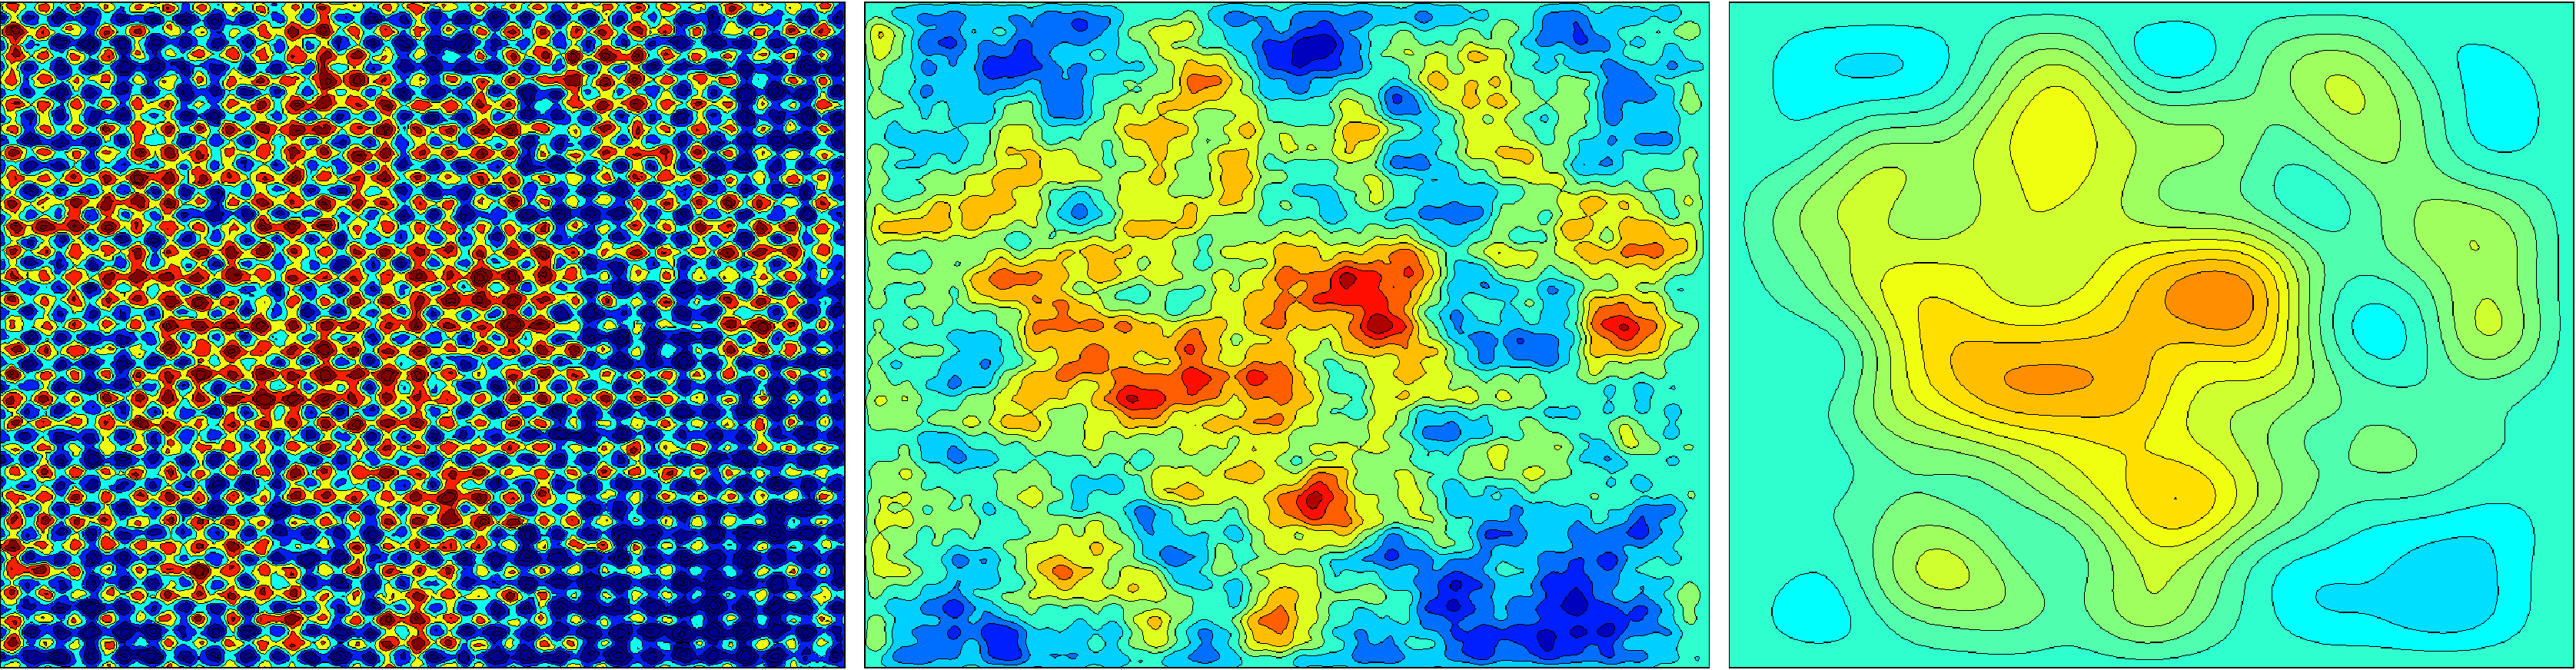
\includegraphics[width=\textwidth]{PSI.pdf}
\caption{1) 2D turbulence with several sinusoidal and random signals as initial condition, 2) at a later time 3) at a much later time. Code from
\cite{Seibold2008a}.}
\end{figure}

%%####################################################################
\begin{turbu}[$\beta$-effect]\label{turb:beta}
Consider at last the inviscid rotating flat-disk-type tank this time in the shape of a shell of a sphere with again $\vec{g} \parallel \vec{z}$ everywhere
perpendicular to the surface at rest. Further assume a strong $\vec{g}$ so that the $\vec{\Omega} \cdot \vec{y}$ component in the Coriolis term is dwarfed by
hydrostaticity. Then with $\vec{f}=f \vec{z} = \left( \vec{\Omega} \cdot \vec{z} \right)\vec{z}$ now from a Eulerian perspective:
%%--------------------------------------------------------------------
\begin{subequations}
	\label{eq:theory6}
\begin{align}
\dpr{\vec{u}}{t}
	&=
-
\vec{u} \cdot \grad \vec{u}
	-
		\vec{f} \times \vec{u}
	+
	g \vec{\nabla} \eta
	\label{eq:NS6} \\
	%%####################################################################
	 \addtocounter{equation}{+1}
	%%####################################################################
\dpr{\vec{\omega}}{t}
	&=
	-\vec{u}_{h} \cdot \grad_{h} \vec{\omega}
	-v \dpr{f}{y}
	\label{eq:vort6}
	%%####################################################################
	%%####################################################################
	%\frac{D \Em}{D t}
	%&=
	%\nu	\left(
	%\frac{1}{2}\grad^2 \vec{u}^2 - \norm{\grad \vec{u}}^2
	%\right)
	%\label{eq:Emech6}\\
	%%%####################################################################
	%%%####################################################################
	%\frac{D \enstro}{D t}
	%&=
	%\vec{\omega}\cdot  \nu \grad^{2} \vec{\omega}
	%\label{eq:enst6}
\end{align}
\end{subequations}


%%--------------------------------------------------------------------
A new term with opposite sign from the $\omega$-advection-term in $y$-direction arises in the vorticity budget, which is evidently most significant where $f$
changes strongest meridionally, \ie In proximity to the sphere's \textit{equator}. Hence, if scales permit, relative vorticity can now also be altered by a
change in latitude via conservation of angular momentum.
\end{turbu}
%%####################################################################
%%####################################################################
% % --------------------------------------------------------------------
% %
%  \chapter{Eddy Categories}
% % --------------------------------------------------------------------
%  \label{chap:eddy_cat}
Starting from the considerations for \eqsref{eq:theory6} and introducing a variable
density, the momentum equations and the
$z$-component of the vorticity equation read:
%%--------------------------------------------------------------------
\begin{subequations}
\begin{align}
	\left(\dpr{\vec{u}}{t}\right)^{\rnm{1}}
	+
	\left(\vec{u} \cdot \grad \vec{u}\right)^{\rnm{2}}
	+
	\left(\vec{f}_{0} \times \vec{u}\right)^{\rnm{3}}
	+
	\left(\beta y \times \vec{u}\right)^{\rnm{4}}
	&=
	\left(- g \grad \h \right)^{\rnm{5}}
	\label{eq:NS7} \\
	%%####################################################################
	%%####################################################################
	\div \vec{u}
	&=
	0 \label{eq:konti7}\\
	%%####################################################################
	%%####################################################################
	\left(\Dpr{\omega}{t}\right)^A
	+
	\left(\Dpr{f}{t}\right)^B
	&=
	\left(f \dpr{w}{z} \right)^C
	+
	\left(\omega \dpr{w}{z} \right)^D \label{eq:vort7}
	%%####################################################################
	%%####################################################################
	%\frac{D \Ek}{D t}
	%&=
	%-
	%\vec{u}_{h} \cdot \frac{1}{\rho} \grad_{h} p
	%+
	%\nu \left(
	%\frac{1}{2}\grad^2 \vec{u}^2 - \norm{\grad \vec{u}}^2
%\right)
	%\label{eq:Ekin1}\\
	%%%####################################################################
	%%%####################################################################
	%\frac{D \Em}{D t}
	%&=
	%\nu	\left(
	%\frac{1}{2}\grad^2 \vec{u}^2 - \norm{\grad \vec{u}}^2
	%\right)
	%\label{eq:Emech1}\\
	%%%####################################################################
	%%%####################################################################
	%\frac{D \enstro}{D t}
	%&=
	%\vec{\omega}\cdot \left( \vec{\vec{\omega}_{a}} \cdot \grad \right) \vec{\vec{u}}
	%+
	%\vec{\omega}\cdot  \nu \grad^{2} \vec{\omega}
	%\label{eq:enst1}
\end{align}
\end{subequations}


%%--------------------------------------------------------------------

Several balances between terms to maintain vortices are thinkable here:

%%####################################################################
%%####################################################################



\begin{eddy}[Frontal Lenses]\label{eddy:FrontalLense}
\begin{description}[noitemsep,nolistsep]
\item[large:]\hspace{50 pt}
 $\Rh$, $\Bu$, U
%\item[$\le 1$:]\hspace{62 pt}
\item[small:]\hspace{50 pt}
$\Ro$, W
\item[balance between:]
$\rnm{2}$, $\rnm{3}$ and $\rnm{5}$
%\item[significant vorticity term:]
%$A$
\end{description}
The case with strong density gradients, large current speeds and a Rossby number approaching unity is typical for the meandering tails of turbulent boundary
currents and zonal jets as in the Gulf Stream respective cyclogenesis in the atmospheric jet stream. Technically the intrathermoclinic lenses
\citep{Cushman-Roisin1990} and strong-density-gradient deep eddies e.g. \textit{meddies} fall into this group as well. With strong stratification, small
vertical displacements cause strong pressure gradients. The dynamics can be limited to some thin layer, bottom topography is of little relevance and the surface
signal might be small, or misleading.
 \end{eddy}
%###################################%


\begin{eddy}[Small Mid-Latitude Geostrophic Eddies] \label{eddy:midlat}
\begin{description}[noitemsep,nolistsep]
\item[large:]\hspace{50 pt}
 $\Rh$
\item[$\mathcal{O} 1$:]\hspace{62 pt}
$\Bu$
\item[small:]\hspace{50 pt}
$\Ro$
\item[balance between:]
$\rnm{3}$ and $\rnm{5}$
%\item[significant vorticity term:]
%none. stationary at first approximation.
\end{description}
The true geostrophic eddy with $L \sim \mathrm{L_R} \sim NH/f$.
\end{eddy}
%%####################################################################
%%####################################################################

\begin{eddy}[Large Geostrophic Gyres] \label{eddy:gyres}
\begin{description}[noitemsep,nolistsep]
%\item[large:]\hspace{50 pt}
%\item[$\mathcal{O} 1$:]\hspace{62 pt}
\item[small:]\hspace{50 pt}
$\Ro$, $\Rh$, $\Bu$
\item[balance between:]
$\rnm{3}$,   $\rnm{4}$, $\rnm{5}$ and friction
%\item[significant vorticity term:]
%$B$, $C$
\end{description}
The large-scale wind-driven ocean gyres. These can only be interpreted as an \textit{eddy} from the Reynolds-averaged large-scale perspective. The motion is strongly $f/H$-contour guided and the $\beta$-effect is immediately apparent in their strong western boundary intensification.
\end{eddy}


%%####################################################################
%%####################################################################
\begin{eddy}[the \textit{Rossby-wave}-eddy] \label{eddy:rossbywave}
\begin{description}[noitemsep,nolistsep]
\item[large:]\hspace{50 pt}
L
\item[$\mathcal{O} 1$:]\hspace{62 pt}
$\Bu$
\item[small:]\hspace{50 pt}
$\Ro$ $\Rh$
\item[balance between:]
$\rnm{3}$,$\rnm{4}$ and $\rnm{5}$
%\item[significant vorticity term:]
%$B$
\end{description}
In low latitudes quasi-geostrophy and hence a small Rossby number demand large
$L$ and/or small $U$. The pressure gradients and hence surface elevation is
small. Due to the large meridional extent, slow time-scale and strong
$f(y)$-gradient, particles moving north or south experience strong changes in
planetary vorticity. So much so, that in this regime geostrophic eddies and
Rossby waves are no longer clearly separable phenomena.
\end{eddy}
%%####################################################################
%%####################################################################


\begin{eddy}[\textit{bonus: tornado}] \label{eddy:tornado}
\begin{description}[noitemsep,nolistsep]
\item[large:]\hspace{50 pt}
$U$, $g'$, $\mathrm{L_R}$ ,$\Ro$, $\Bu$, $\Rh$
\item[small:]\hspace{50 pt}
$L$
\item[balance between:]
$\rnm{2}$ and $\rnm{5}$
\item[significant vorticity term:]
$A$ and friction (not considered here)
\end{description}\vspace{2pt}
This case isn't really applicable to the ocean except for maybe the tropics where $f$ vanishes (but $\nu$ would become relevant) or on small scales in areas of strong tidal currents in combination with bathymetry \ie \textit{tidal bores} etc . In this case a pressure force would have to be balanced by a centrifugal force alone (\eg \textit{bathtub}).
\end{eddy}







% % --------------------------------------------------------------------
% %
% %
% \chapter{Further Papers}
% % --------------------------------------------------------------------
%  

\section*{\citealt{gent1990isopycnal,gent1995parameterizing}}\label{sec:hist_gentmcw}
\citeauthor*{gent1990isopycnal} set the foundation for today's standard parametrization of eddy-mixing in non-eddy-resolving general circulation models \footnote{general circulation models will hereafter be abbreviated GM.}.
Essentially, they argue that a plain Fickian diffusion-type parametrization of
the form $K \grad \vec{u}$ is inadequate since $\vec{u}$ only represents the
large-scale flow.
Instead the relevant velocity for eddy-diffusion is the sum of mean flow and eddy-induced flow \footnote{which will hereafter be called \textit{bolus velocity} in line with \cite{rhines1982basic} who coined the term} $\vec{U}=\ol{\vec{u}} + \ol{h'_{\rho} \vec{u}'}/\ol{h_{\rho}} =\ol{\vec{u}} + \vec{u}^{\star}$ with $h(x,y,\rho,t)$ as the physical height of an isopycnal and $h_{\rho}$ the equivalent in isopycnal coordinates and $\Dprs{}{t}= \dpr{}{t} +\vec{U} \grad $ as the material derivative with respect to $\vec{U}$ instead of $\vec{u}$.
In their assumption, analogous to adiabatic eddy mixing of passive tracers, the  turbulence, itself \textit{sitting adiabatically} on the large scale density surfaces, redistributes thickness anomalies \textit{quasi-adiabatically} along \textit{quasi}-neutral surfaces. \Ie the integrated turbulent eddy activity effectively smears large-scale density gradients at the rate of the bolus velocity, akin to a Fickian diffusion of a passive tracer. With the momentum equations reduced to the large-scale, inviscid, incompressible and stationary, the entire dynamics can be represented via the prognostic advection-diffusion equation for $h_{\rho}$: \todoil{solve for h instead of rho in mass budget}\\
%%....................................................................
\begin{subequations}\begin{align}
	\rho_0  f \vec{k} \times \vec{u}
	&=
	-\grad p\\
	%%--------------------------------------------------------------------
	\Dprs{\rho}{t} % = \dpr{\rho}{t} + \vec{U} \cdot \grad^{\star} \rho
	&=
	0 \\
	%%--------------------------------------------------------------------
	\grad^{\star} \cdot \vec{U}^{\star}
	&=
	0	\\
	%%--------------------------------------------------------------------
	 \addtocounter{equation}{+3}
	h \Dprs{\tau}{t}
	&=
	 \left(\grad \cdot \left( h\mu \grad \tau \right) \right)^{\star}	\label{eq:fick_tracer}\\
 \vec{u}_h^{\star} &= \dpr{}{z}\left( K \grad \rho/\dpr{\rho}{z} \right) \\
w^{\star} &=-\div\left( K \grad \rho/\dpr{\rho}{z} \right)
\end{align}\end{subequations}
%%....................................................................
\Eqref{eq:fick_tracer} is the tracer equation with $\mu$, analogous to $K$, as an unknown diffusion coefficient and all $\star$ indicating a transformation to the isopycnal frame of reference.
 If $K$ is taken as constant the potential vorticity equation reduces to
%%....................................................................
\begin{align}
	\Dprs{f\partial \rho / \partial z}{t}
	&=
	K \grad_{\rho} \cdot \left( f h_{\rho} \grad_{\rho} \dpr{\rho}{z} \right) /h_{\rho} \label{vort-diff}
%%%--------------------------------------------------------------------
	%&=
	%K \left(
%f \grad^2_{\rho} \dpr{\rho}{z}
%+ 	\grad \left( f h_{\rho}\right) \cdot	  \grad_{\rho} \dpr{\rho}{z} /h_{\rho}\right) \\
  %%%-------------------------------------------------------------------
	%&=
		%K \left(
%f  \grad^2_{\rho} h_{\rho}^{-1}
%+ 	\grad \left( f h_{\rho}\right) \cdot	h^{-1}_{\rho}  \grad_{\rho} h_{\rho}^{-1} \right) \\
  %%%-------------------------------------------------------------------
	%&=
		%K \left(
%f  \grad^2_{\rho} h_{\rho}^{-1}
%+ 	\grad \left( f h_{\rho}\right) \cdot	  \grad_{\rho} h_{\rho}^{-2}/2 \right) \\
	%&=
		%K \left(
%f  \grad^2_{\rho} h_{\rho}^{-1}
%+ 	 f\grad \left( h_{\rho}\right) \cdot	  \grad_{\rho} h_{\rho}^{-2}/2
%+ h_{\rho}	\grad \left( f \right) \cdot	  \grad_{\rho} h_{\rho}^{-2}/2 \right) \\
\end{align}
%%....................................................................
\todoil{reminiscent of QPVE, try again later..}.Hence under the assumption of
exact Fickian thickness diffusion, potential vorticity is diffused as if it were
a passive tracer, too. Intuitively this sounds absurd and counter-Newtonian
since vorticity is intrinsically linked to velocity itself. It must be kept in
mind though, that this diffusion stems solely from the bolus velocity, the
vorticity of which is only a fraction of the vorticity of the mean state. On
scales much larger than the baroclinic Rossby radius, the baroclinic eddy
dynamics are so far decoupled from the mean barotropic flow in terms of their
scales that, in this assumption, they simply drift along on it, unaffected. In
other words, from a frame of reference that is advected with the mean flow, the
eddy-induced dynamics are assumed to have a large ratio of local to pseudo
forces.
Nevertheless, aforementioned simplification does indeed technically violate
conservation of angular momentum \citep{Rhines2006}.

%with
%%%....................................................................
%\begin{align}
%\mathbf{K}
%=
%\left[
	%\begin{array}{c@{}c@{}}
		%\left[\begin{array}{cc}
			%1 & 1 \\
			%1 & 1 \\
		%\end{array}\right] & \mathbf{L}  \\
		%\mathbf{L}^{T} & \mathbf{L}^{2}
	%\end{array}
%\right];
%\;\;\;\;  -\mathbf{L}
%=
%\frac{\grad \rho}{\partial \rho / \partial z}
%\end{align}
%%%....................................................................
%%%....................................................................
%\begin{align}
%-\mathbf{L}
%&=
%\frac{\grad \rho}{\partial \rho / \partial z}
%\end{align}
%%%....................................................................




\section*{\citealt{larichev1995eddy}}\label{sec:hist_lari95}
\citeauthor{larichev1995eddy} investigated vorticity-fluxes in $k$-space  using a simple two-layer quasi-geostrophic model with domain dimensions much larger $\Lr$, in order to avoid a scale limiting basin-size. Their finding is that, contrary to theory, that predicts a flux of baroclinic potential vorticity from large scales where it is excited down-gradient to $\Lr$ where it feeds into the barotropic mode, and thence back up the red cascade, both energy production and strongest vorticity fluxes are strongest towards the largest scales of the flow and not at $\Lr$. They therefore argue that instead of concentrating on eddies at scale $\Lr$, focus should really be on the largest scale the inverse cascade extends to, be that an arrest scale via $\beta$ or via some threshold beyond which eddies abandon turbulent regions, by for instance the effects outlined by \cite{Cushman-Roisin1990}.



\section*{\citealt{scott2005direct}}\label{sec:hist_wang}
\cite{wunsch1996ocean} argues that SSH-variability is mostly representative of
the first baroclinic mode since, under the assumption that kinetic energy be
roughly equally partitioned between barotropic and baroclinic mode, the first
baroclinic mode, being representative of strong density gradients, is primarily
concentrated towards the surface \citep{scott2005direct}.\\
Geostrophic turbulence theory predicts an inverse cascade for the barotropic mode, yet a direct cascade for the first baroclinic mode from large scales towards $\Lr$ \citep{vallis2006atmospheric}  \todo[color=red]{maybe show derivation from vallis...}. Hence satellite SSH-products should show a direct cascade in regions of excitations of geostrophic turbulence on scales larger than $\Lr$.
Curiously, evidence of the opposite was found by \eg \cite{tapley1994accuracy,Kobashi2002}, somewhat affirming the findings of \cite{larichev1995eddy}. \cite{scott2005direct} therefore argue that \textit{Because the growth in scale is extending well beyond $2\pi\Lr$, especially for the zonal velocity, even in these subtropical regions \footnote{with reference to \cite{Kobashi2002}}, we claim there is an unresolved, and indeed unappreciated, contradiction between stratified geostrophic turbulence theory and observations. Furthermore, \cite{Kobashi2002} also claim to observe the eddies evolving into zonally elongated, wavelike structures, as predicted by \cite{Rhines2006}. But again, theory holds this to be a barotropic mode phenomenon that does not apply to the baroclinic modes.}
With regard to the last point \cite{scott2005direct} suggest that the apparent arrest may arise from \textit{barotropization, which transfers the energy down the water column, reducing the surface signal}. \todo[color=red]{ ref to here later - argument for further tracking depth }

%%####################################################################
%%####################################################################
\section*{\citealt{Eden2007}}\label{sec:hist_eden07}
\citeauthor*{Eden2007} inferred eddy scales in the north-Atlantic from kinetic energy densities in $k$-space and spatial decorrelations. They detect two different regimes that are meridionally separated by $\Lr=\Lb$. South of this dividing line, they find small-Rhines-number-type anisotropic scales, whereas the scales due north show proportionality to the Rossby-radius. They therefore suggest to use $L=min(\Lb,\Lr)$ instead of $\Lr$ as the characteristic length scale in parametrizations.
This meridional wave/eddy-dualism was already proposed by \cite{rhines1979theoretical}, who noted that the $\Lb$ becomes important when the phase speed at which Rossby waves displace particles is of same order as the turbulent velocity scale, \ie when $U \sim \beta\Lr^2$ and hence $U/\beta = \Lb^2 \sim \Lr^2$. Or quoting \cite{Tulloch2009}: \textit{The central idea of the Rhines effect is that, as eddies grow in the inverse cascade, their timescale slows, and when this timescale matches the frequency of Rossby waves with the same spatial scale, turbulent energy may be converted into waves, and the cascade will slow tremendously}

%%####################################################################
%%####################################################################

\section*{\citealt{Eden2006,Eden2007a,eden2008towards}}\label{sec:hist_eden-K}
Theoretically the approximated, parametrized equations can be solved for the
thickness diffusivity $K$, which can then be determined from \eg fine-grid model
results. One problem with this is that it is only the along-gradient component
of the flux that is of interest. However the cross-gradient term proportional to
$\vec{k}_h \times \grad_h \rho_h$  integrates to non-zero in the parametrization
when anisotropic fluxes are considered. This term is mute to the tracer budget
as it has ,by definition, zero divergence and is thus not necessary in the
parametrization and in general assumed to be zero. It does however affect the
opposite operation of estimating $K$ from data.
Ignoring this term results in negative thickness diffusivities in regions where \eg eddies merge back into jets or more more general anywhere where the transfer of mean potential energy to eddy kinetic energy is reversed. If one were to interpret the thickness flux in direct analogy to the frictional term in the momentum equations, negative $K$ would be analogous to a negative viscosity \ie a reversal of a diffusive process and one would run into complications regarding fundamental thermodynamic principles. After all a negative $K$ is physically implausible in light of the general assumption that $K\sim U L$. \\
\citeauthor{Eden2006,Eden2007a,eden2008towards} decomposed $K$ into its along
and cross gradient component and calculated their values from model data with
emphasis on the southern ocean. It turns out that the rotational component is
indeed significant at the outer flanks of the ACC \ie in regions of strong
interaction between mean flow and eddies.
\citeauthor{Eden2006,Eden2007a,eden2008towards} also indicate that the adiabatic
assumption is unrealistic in proximity to the mixed layer where eddies also
induce significant diapycnal fluxes in depths that are substantially influenced
by \eg the surface heat flux.

%%####################################################################
%%####################################################################

\section*{\citealt{Tulloch2009}}\label{sec:hist-tulloch}
As noted in \ref{sec:hist_killworth}, interpreting SSH-signals in terms of long
Rossby waves results in a discrepancy in observed and predicted phase speeds.
\cite{Tulloch2009} therefore flipped the chain of arguments by fitting
quasi-geostrophic theory to observed phase speeds and correcting for mean-flow
Doppler shifts, thereby setting constraints on the possible wave lengths and
vertical structure. Furthermore they use climatological mean velocity and
density data to construct the vertical eigenfunctions for the
long-wave-dispersion-relation and then extract the vertical profiles of the
observed velocities, assuming that they project entirely onto the first
baroclinic mode \footnote{see \cite{wunsch1996ocean}}. This way they can scale
observed $u_{rms}(z)$ from drifter data by their respective factor from the
vertical mode. The resultant corrected velocities and scales are in approximate
agreement with \cite{Eden2006b} and \cite{Chelton2007}. They conclude that the
vast majority of the mid- to high-latitude
world ocean is baroclinically unstable and characterized by an inverse energy cascade fed by geostrophic turbulence at deformation scale. In Regions characterized by small Rhines number, on the other hand, the turbulence eventually grows to Rhines scale where it blends in with Rossby waves.


%\section*{\citealt{Smith2009}}\label{sec:hist-smith}


\section*{\citealt{Eden2011a,eden2012implementing,Vollmer2013a}}\label{sec:hist_eden-linstab}
A linear stability analysis is particularly suitable for the analysis of eddy
diffusivities since it describes deviations from a mean state, by definition.
Linearizing the quasi-geostrophic stream function about a laterally
\textit{quasi}-constant \footnote{\textit{quasi} in the sense that \eg
\citeauthor*{Vollmer2013a} allowed for horizontal variations of the mean state
iteratively via a WKBJ approximation.} mean state \ie applying a perturbation
ansatz to the equations leads to a vertical Sturm-Liouville-type eigenvalue
problem. Motivated by the work of \cite{Smith2007},
\citeauthor{Eden2011a,eden2012implementing,Vollmer2013a} rigorously solved the
problem for its vertical modes and derived values for buoyancy and potential
vorticity diffusivities for either the world ocean or specific regions of
interest.  They construct the amplitude of the resultant perturbation stream
function as a linear function of the imaginary part of the phase speed and the
wavelength of the fastest growing mode, scaled by a
constant parameter, suggested to link the length scales of unstable wave and resultant eddy \footnote{the difference is assumed to be a result of the inverse cascade.}. One of their most interesting findings is that a zonal mean flow has two main effects on eddy diffusivities:
\begin{itemize}
	\item
	An eastward flow and a positive shear ($\dpr{\ol{u}}{y}$) decrease skew diffusivity\footnote{\ie the rotational part of thickness diffusivity as mentioned in \ref{sec:hist_eden07}} $\tsca{K}$  and shift it along with the steering level down vertically.
	\item
	A westward flow and negative shear effect the opposite.
	\item
	A large $\beta$ also intensifies $\tsca{K}$ towards the surface.
\end{itemize}
All of this makes intuitively sense. $\tsca{K}$ is only non-zero when total
thickness-diffusivity is anisotropic \ie when net turbulence does not cancel out
laterally. This happens when eddies prefer one direction over another. As was
shown by \cite{Cushman-Roisin1990} meso-scale eddies need to always migrate west
in order to balance forces symmetrically. This is why they have shorter life
times and a tendency to hide at depth in the ACC and why values for $\tsca{K}$
are large in the strongly vertically stratified ($\dpr{\ol{u}}{z}<0$) westward
equatorial current.





% % --------------------------------------------------------------------
% %
% \chapter{Derivations}
% %\begin{multicols}{2}


\begin{derivation}[Vorticity]\label{der:vort}
	With the identity
	%%--------------------------------------------------------------------
	\begin{equation}\begin{split}
	\vec{u} \cdot \grad \vec{u}
	&=
	\left( \grad \times  \vec{u}  \right)\times \vec{u}
	+ \grad \vert \vec{u}\vert ^{2}/2\\
	&=
	\omega \times \vec{u}
	+ \grad \vec{u}^{2}/2
	\end{split}\end{equation}
	\eqref{eq:NS2} becomes
	%%--------------------------------------------------------------------
	\begin{equation}\begin{split}
	\frac{\partial \vec{u}}{\partial t}
	+
	\grad \vert \vec{u}\vert ^{2}/2
	+
	\left( 2\vec{\Omega} + \vec{\omega} \right)  \times \vec{u}
	&=
	- \frac{1}{\rho} \vec{\nabla} p
	+
	\nu  \vec{\nabla}^{2} \vec{u}
	+
	\vec{g} \\
	\frac{\partial \vec{u}}{\partial t}
	+
	\grad \vert \vec{u}\vert ^{2}/2
	+
	\vec{\omega_{a}} \times \vec{u}
	&=
	- \frac{1}{\rho} \vec{\nabla} p
	+
	\nu  \vec{\nabla}^{2} \vec{u}
	+
	\vec{g}
	\end{split}\end{equation}
	%%--------------------------------------------------------------------
	Applying the curl operation to \eqref{eq:NS2} and assuming \eqref{eq:konti1}
	for	an incompressible fluid yields and equation for the vorticity
	%%--------------------------------------------------------------------
	\begin{equation}\begin{split}
	&\frac{\partial \vec{\omega}}{\partial t}
	+
	\curl \grad \vert \vec{u}\vert ^{2}/2
	+
	\curl \left( \omega_{a} \times \vec{u} \right) \\
	&=
	-\frac{1}{\rho} \curl \grad p
	-
	\grad \rho^{-1} \times \grad p
	+
	\nu \grad \times \grad^{2} \vec{u}
	+
	\grad \times \vec{g} \label{eq:vort1}
	\end{split}\end{equation}
	%%--------------------------------------------------------------------
	Annihilating all $\curl \vec{grad}$ and $\div \curl$ and making use of
	the
	identity
	%%--------------------------------------------------------------------
	\begin{equation}\begin{split}
	\grad \times \left( \vec{A} \times B \right)
	&=
	\vec{A} \left( \grad \cdot B \right)
	-
	B \left( \grad \cdot \vec{A} \right)
	+
	\left( B \cdot \grad \right) \vec{A}
	-
	\left( \vec{A} \cdot \grad \right) B
	\end{split}\end{equation}
	%%--------------------------------------------------------------------
	%%--------------------------------------------------------------------
	\eqref{eq:vort1} becomes
	%%--------------------------------------------------------------------
	\begin{equation}\begin{split}
	\frac{\partial \vec{\omega}}{\partial t}
	+
	\curl \left( \omega_{a} \times \vec{u} \right)
	&=
	-\frac{\grad \rho \times \grad p	}{\rho^{2}}
	+
	\nu \grad \times \grad^{2} \vec{u}\\
	%%--------------------------------------------------------------------
	\frac{\partial \vec{\omega}}{\partial t}
	+
	\left( \vec{\vec{u}} \cdot \grad \right) \vec{\vec{\omega}_{a}}
	-
	\vec{\vec{u}} \left( \grad \cdot \vec{\vec{\omega}_{a}} \right)
	&-
	\left( \vec{\vec{\omega}_{a}} \cdot \grad \right) \vec{\vec{u}}\\
	&=
	\B
	-
	\nu \curl \left( \curl \left( \curl \vec{u} \right) \right)\\
	%%--------------------------------------------------------------------
	\frac{D \vec{\omega_{a}}}{D t}
	&=
	\left( \vec{\vec{\omega}_{a}} \cdot \grad \right) \vec{\vec{u}}
	+
	\B
	-
	\nu \curl \left( \curl \omega \right)\\
	&=
	\left( \vec{\vec{\omega}_{a}} \cdot \grad \right) \vec{\vec{u}}
	+
	\B
	+
	\nu \grad^2 \vec{\omega}
	\end{split}\end{equation}
	Scaling considerations based on the small aspect ratio e.g. noting that
	$\B \sim \grad p \times \grad \rho$ is at first approximation
	limited to	the $x,y$ plane and that $U/H \gg W/L$ and assuming $\omega_z
	\gg	\omega_h $,	leads to:

	%%%....................................................................
	\begin{equation}\begin{split}
	\dpr{\vec{\omega} }{t}
	+
	\advec{\vec{\omega}}
	+
	\beta v \unitvec{z}
	&=
	\left(\omega_z +
	f\right) \dpr{ \vec{u}}{z}
	+
	\B
	%%--------------------------------------------------------------------
	\end{split}\end{equation}
	horizontal:
	\begin{equation}\begin{split}
	&\frac{1}{T} \frac{U}{H }
	+
	\left(\frac{U }{L} + \frac{W}{H} \right)
	\frac{U }{H}
	\sim
	\frac{U }{H} \frac{U}{L}
	+
	f \frac{U}{H}
	+
	\B \\
	\Rightarrow
	&\frac{U}{HT }
	+
	\frac{U^2 }{LH}
	+
	\frac{UW }{H^2}
	\sim
	\frac{U^2}{LH}
	+
	f \frac{U}{H}
	+
	\B
	%%--------------------------------------------------------------------
	\end{split}\end{equation}
	vertical:
	\begin{equation}\begin{split}
	&\frac{U}{LT}
	+
	\frac{U^2}{L^2}
	+
	\frac{W U}{ H L}
	+
	\beta V
	\sim
	\frac{UW}{LH}
	+
	f\frac{W}{H}
	\\
	\Rightarrow
	&\frac{U}{LT}
	+
	\frac{U^2}{L^2}
	+
	\beta V
	\sim
	\frac{WU}{HL}
	+
	f\frac{W}{H}
	\end{split}\end{equation}
	%%%....................................................................

	Hence at first order:
	\begin{equation}\begin{split}
	\Dpr{\vec{\omega}_h }{t}
	&=
	\left(f + \omega_z \right)\dpr{\vec{u}_h}{z}
	+
	\B
	\end{split}\end{equation}
	\begin{equation}\begin{split}
	\Dpr{\omega_z }{t}
	+
	\beta v
	&=
	\left(f + \omega_z \right)\dpr{w}{z}
	\end{split}\end{equation}
	%If we further assume quasi-geostrophic motion so that any change in
	$\vec{\omega}_h$ is due to small ageostrophic parallelization of $\grad p$
	and	$\grad \rho$  via $B$ the tilting terms vanish, since then
	$\vec{\omega}_h$	normal to the plane spanned by $\grad \vec{u}_h$ and
	$\grad	w$
\end{derivation}

%%####################################################################
%%####################################################################


\begin{derivation}[Kinetic Energy]\label{der:Ek}
Multiply \eqref{eq:NS2} by $ \vec{u}$:
\begin{equation}\begin{split}
\vec{u} \cdot{}
\left(
\frac{\partial \vec{u}}{\partial t}
+
\vec{u}\cdot \grad \vec{u}
+
2\vec{\Omega} \times \vec{u}
\right)
&=
-
\vec{u} \cdot \frac{1}{\rho} \vec{\nabla} p
+
\vec{u}\cdot \nu  \vec{\nabla}^{2} \vec{u}
+
\vec{u}\cdot  \vec{g}\\
%%--------------------------------------------------------------------
\frac{1}{2}\frac{\partial \vec{u}^{2}}{\partial t}
+
\frac{1}{2}  \vec{u}\cdot \grad \vec{u}^{2}
+
\vec{u} \cdot 2\vec{\Omega} \times \vec{u}
&=
-
\vec{u} \cdot \frac{1}{\rho} \vec{\nabla} p
+
\vec{u}\cdot \nu  \vec{\nabla}^{2} \vec{u}
-
w g \\
%%--------------------------------------------------------------------
\frac{1}{2}\frac{\partial \vec{u}^{2}}{\partial t}
+
\frac{1}{2}  \vec{u}\cdot \grad \vec{u}^{2}
&=
-
\vec{u}_{h} \cdot \frac{1}{\rho} \grad_{h} p
+
w g
+
\vec{u}\cdot \nu  \vec{\nabla}^{2} \vec{u}
-
w g \\
%%--------------------------------------------------------------------
\frac{1}{2}\frac{\partial \vec{u}^{2}}{\partial t}
+
\frac{1}{2}  \vec{u}\cdot \grad \vec{u}^{2}
&=
-
\vec{u}_{h} \cdot \frac{1}{\rho} \grad_{h} p
+
\vec{u}\cdot \nu  \vec{\nabla}^{2} \vec{u} \\
%%--------------------------------------------------------------------
\frac{\partial \Ek}{\partial t}
+
\vec{u}\cdot \grad \Ek
&=
-
g \vec{u}_{h} \cdot  \grad \eta(x,y)
+
\nu\left(
\frac{1}{2}\grad^2 \vec{u}^2 - \norm{\grad \vec{u}}^2
\right)
\end{split}\end{equation}
\end{derivation}

%%####################################################################
%%####################################################################

\begin{derivation}[Mechanical Energy]
\label{der:Em}
Add term for potential energy to \eqref{eq:Ekin1} (assuming $\grad \rho=0$)
\begin{equation}\begin{split}
\frac{D E_{m}}{D t}
&=
-
g \vec{u} \cdot  \grad \eta(x,y)
+
\nu\left(
\frac{1}{2}\grad^2 \vec{u}^2 - \norm{\grad \vec{u}}^2
\right)
+
\vec{u}\cdot\vec{g}\\
%%--------------------------------------------------------------------
\frac{D E_{m}}{D t}
&=
-
g \vec{u} \cdot  \grad \eta(x,y)
+
\nu\left(
\frac{1}{2}\grad^2 \vec{u}^2 - \norm{\grad \vec{u}}^2
\right)
-wg\\
%%--------------------------------------------------------------------
&=
-
g \left( \frac{\partial \eta}{\partial t}
+
\vec{u} \cdot  \grad \eta \right)
+
\nu\left(
\frac{1}{2}\grad^2 \vec{u}^2 - \norm{\grad \vec{u}}^2
\right)\\
%%--------------------------------------------------------------------
&=
-
g \frac{D \eta}{D t}
+
\nu\left(
\frac{1}{2}\grad^2 \vec{u}^2 - \norm{\grad \vec{u}}^2
\right)\\
%%--------------------------------------------------------------------
&=
\nu\left(
\frac{1}{2}\grad^2 \vec{u}^2 - \norm{\grad \vec{u}}^2
\right)
\end{split}\end{equation}
\end{derivation}


%%####################################################################
%%####################################################################

\begin{derivation}[Enstrophy]
\label{der:enstro}
In 2 dimensions the definition of enstrophy can also be rewritten as:
%%%....................................................................
\begin{equation}\begin{split}
\Enstro
=
\inta{\enstro}
&=\inta{
\norm{\grad \vec{u}}^2}
\\
&=\inta{
\left(\frac{\partial v}{\partial x}\right)^2
+ \left(\frac{\partial u}{\partial y} \right)^2
+\left(\frac{\partial v}{\partial y}\right)^2
+ \left(\frac{\partial u}{\partial x} \right)^2}
\\
&=\inta{
\left(\frac{\partial v}{\partial x}\right)^2
+ \left(\frac{\partial u}{\partial y} \right)^2
+\left(\frac{\partial v}{\partial y}\right)^2
+ \left(\frac{\partial u}{\partial x} \right)^2
-\left(\div \vec{u}\right)^{2}}
\\
&=\inta{
\left(\frac{\partial v}{\partial x}\right)^2
+ \left(\frac{\partial u}{\partial y} \right)^2
-2 \dpr{u}{x}\dpr{v}{y}
}
\\
&=\inta{
\omega^{2}
+2 \dpr{u}{y}\dpr{v}{x}
-2 \dpr{u}{x}\dpr{v}{y}
}\\
&=\inta{
\omega^{2}
+2 \dpr{u}{y}\dpr{v}{x}
+2 \left(\dpr{v}{y} \right)^2
}
\end{split}\end{equation}
with $\div \vec{u}=0$ and appropriate boundary conditions, the last two
terms	cancel in the integral leaving

\begin{equation}\begin{split}
\Enstro
&=\inta{
\omega^{2}
}
\end{split}\end{equation}

\end{derivation}

%%####################################################################
%%####################################################################

\begin{derivation}[Vorticity Scales]
\label{der:vortscale}
Assuming approximate geostrophy and $\Bu = \order{1}$:
%%%....................................................................
\begin{equation}\begin{split}
\rho fU
&\sim
\grad p
\end{split}\end{equation}
%%%....................................................................
in a layered model:
%%%....................................................................
\begin{equation}\begin{split}
fU
&\sim
g' \grad \eta \\
U
&\sim
\frac{h N^{2}}{f} \grad \eta \\
U
&\sim
\frac{h^{2} N^{2}}{f\mathrm{L}}
\end{split}\end{equation}
%%%....................................................................
and hence
%%%....................................................................
\begin{equation}\begin{split}
\vec{\omega}
\sim
U/\mathrm{L}
&\sim
\frac{h^{2} N^{2}}{f\mathrm{L}^{2}} \\
&=
\frac{h^{2} N^{2}}{f\mathrm{\Lr}^{2}} \frac{\Lr}{L}\\
&=
f\frac{\Lr}{L}
\end{split}\end{equation}
%%%....................................................................
\end{derivation}
%###################################%\\%###################################%

\begin{derivation}[vortex limitations]
%%%....................................................................
\begin{equation}\begin{split}
\advec{\vec{u}}
+
f \tvec{u}
&=
-g \grad \eta
\end{split}\end{equation}
%%%....................................................................
\begin{equation}\begin{split}
\frac{U^{2}}{L}
+
f U
+
\frac{gh}{L}
&=
0 \\
U^{2}
+
f LU
+
gh
&=
0 \\
\end{split}\end{equation}
%%%....................................................................
possible balances:
%%%....................................................................
cyclone\\$\sign{F_{c}}=\sign{F_{p}}$:
\begin{equation}\begin{split}
U_{1,2}
&=
-fL/2
\pm
\sqrt
{
f^{2}L^{2}/4
+
gh
}
\end{split}\end{equation}
%%%....................................................................
%%%....................................................................
anti-cyclone\\
$\sign{F_{c}}=-\sign{F_{p}}$:
\begin{equation}\begin{split}
U_{1,2}
&=
-fL/2
\pm
\sqrt
{
f^{2}L^{2}/4
-
gh
}
\end{split}\end{equation}

%%%....................................................................
\begin{equation}\begin{split}
4g h
&\le
f^{2}L^{2}\\
2c
&\le
fL\\
2 \mathrm{L_{R}}
&\le
L\\
\end{split}\end{equation}
%%%....................................................................
\end{derivation}

%%####################################################################
%%####################################################################

\begin{derivation}[Okubo-Weiss-Parameter]\label{der:okubo}
%%%....................................................................
\begin{equation}\begin{split}
\ten{T}
&=
\grad \vec{u}\\
%%--------------------------------------------------------------------
&=
\dpr{u_i}{x_j} \unitvec{e}_i \unitvec{e}_j \\
&=
\frac{1}{2}\left(
\left(\ten{T}+\tent{T}\right)
+
\left( \ten{T} - \tent{T} \right)
\right) \\
%%--------------------------------------------------------------------
&=
\frac{1}{2} \left( \left( \dpr{u_i}{x_j} + \dpr{u_j}{x_i}\right)
\unitvec{e}_i	\unitvec{e}_j \right)
+
\frac{1}{2} \left( \left( \dpr{u_i}{x_j} - \dpr{u_j}{x_i}\right)
\unitvec{e}_i	\unitvec{e}_j \right)
\end{split}\end{equation}
%%%....................................................................
%%%....................................................................
\begin{equation}\begin{split}
\mathrm{O_w}=\tr{\ten{T}^2}
&=
\left(
\dpr{u_i}{x_k} \dpr{u_k}{x_j} \unitvec{e}_i \unitvec{e}_j
\right)_{i,i}\\
&=
\dpr{u_i}{x_j} \dpr{u_j}{x_i}\\
%%--------------------------------------------------------------------
&=
\left(\dpr{u_i}{x_i}\right)^2
+\left(1-\delta_{i,j}\right)\dpr{u_j}{x_i} \dpr{u_i}{x_j} \\
%%--------------------------------------------------------------------
&=
\left(\dpr{u_i}{x_i}\right)^2
+
\frac{1}{2}\left( \dpr{u_i}{x_j} + \dpr{u_j}{x_i} \right)^2
-\frac{1}{2}\left( \dpr{u_i}{x_j} - \dpr{u_j}{x_i} \right)^2 \\
%%--------------------------------------------------------------------
&=
\frac{1}{2}\left( \dpr{u_i}{x_i} + \dpr{u_j}{x_j} \right)^2
+\frac{1}{2}\left( \dpr{u_i}{x_i} - \dpr{u_j}{x_j} \right)^2
+
\frac{1}{2}\left( \dpr{u_i}{x_j} + \dpr{u_j}{x_i} \right)^2
-\frac{1}{2}\left( \dpr{u_i}{x_j} - \dpr{u_j}{x_i} \right)^2 \\
%%--------------------------------------------------------------------
&=
divergence^2
+ stretching^2
+ shear^2
- vorticity^2
\end{split}\end{equation}
Hence for motion dominated by deformation and shear the system has
hyperbolic	character, whereas vorticity-dominated motion has parabolic
character. Of interest should therefor not only be the value of $\mathrm{O_w}$
but also its	gradient. An abrupt change in $\mathrm{O_w}$ clearly identifies
regions of	vorticity genesis and decay.
\\ In 2 dimensions:
%%%....................................................................
\begin{equation}\begin{split}
\okubo
&=
\left(\dpr{u}{x}\right)^2
+
2 \dpr{u}{y} \dpr{v}{x}
\end{split}\end{equation}
%%%....................................................................
\end{derivation}

%%####################################################################
%%####################################################################
\begin{derivation}[Cushman's Drift Speed]

%%%....................................................................
\begin{equation}\begin{split}
X_t
&=
-\frac{\beta g'}{f_0^2} \frac{\int H\eta + \eta^2/2 \; \mathrm{d}A}{\int\eta \; \mathrm{d}A}\\
&=
-\frac{\beta g'}{f_0^2} \left(H +\frac{ \int  \eta^2/2 \; \mathrm{d}A}{\mathrm{V_e}} \right) \\
&=
-\frac{\beta c^2}{f_0^2} \left(1 +\frac{1}{H} \frac{ \int  \eta^2/2 \;\mathrm{d}A	}{\mathrm{V_e}} \right) \\
&=
-\beta \Lr^2 \left(1 +\frac{1}{H} \frac{ \int  \eta^2 \; \mathrm{d}A}{2\mathrm{V_e}} \right) \\
&=
\frac{\omega_{long}}{k} \left(1 +\frac{1}{H} \frac{ \int  \eta^2 \;\mathrm{d}A}{2\mathrm{V_e}} \right) \\
\end{split}\end{equation}
%%%....................................................................
\end{derivation}

%###################################%\\%###################################%
\begin{derivation}[Mean Fields of $u$ and $b$]
\label{der:fields}
%%%................................................................
\begin{subequations}\label{eq:inhomo1}
\begin{align}
\dpr{u_i}{t} \unitvec{e}_i
+
u_j \dpr{u_i}{x_j}\unitvec{e}_i
+
\delta_{j3}\timesES{f}{u}
&=
-\dpr{p}{x_i}	\unitvec{e}_i
+ \nu \dpr{^2u_i}{x_j^2}\unitvec{e}_i
- \delta_3 g\unitvec{e}_i \label{eq:inhomoNS}\\
% --------------------------------------------------------------------
\dpr{u_i}{x_i}
&=
0 \label{eq:inhomoCON}\\
% --------------------------------------------------------------------
\Dpr{\rho}{t}
&=
-\dpr{J_{i}^{rad}}{x_i}
+   \kappa \dpr{^2 \rho}{x_i} \label{eq:inhomoSTATE}
\end{align}
\end{subequations}
% %%....................................................................
A Reynolds decomposition of \eqsref{eq:inhomo1} yields
% %%....................................................................
\begin{subequations} \label{eq:inhomoDECOMP}
\begin{align}
\begin{split}
\dpr{\inbr{\decom{u_i}}}{t}\unitvec{e}_i
+
\inbr{\decom{u_j}} \dpr{\inbr{\decom{u_i}}}{x_j}\unitvec{e}_i
+
\delta_{j3}\timesES{f}{\inbr{\decom{u}}}\\
=
-\dpr{\inbr{\decom{p}}}{x_i}	\unitvec{e}_i
+ \nu \dpr{^2\inbr{\decom{u_i}}}{x_j^2}\unitvec{e}_i
- \delta_3 \ol{g} \unitvec{e}_i\label{eq:decompfin}
&\end{split}\\
% --------------------------------------------------------------------
\dpr{\inbr{\decom{u_i}}}{x_i}
=
0 & \\
% --------------------------------------------------------------------
\dpr{\inbr{\decom{\rho}}}{t}
+	\inbr{\decom{u_i}}\dpr{\inbr{\decom{\rho}}}{x_i}
=
-	\ol{\dpr{J_{i}^{rad}}{x_i}}
-	\dpr{J_{i}^{rad}}{x_i}'
+   \kappa \dpr{^2 \inbr{\decom{\rho}}}{x_i}
\end{align}
\end{subequations}
% %%....................................................................
Averaging \eqsref{eq:inhomoDECOMP} yields
% %%....................................................................
\begin{subequations}
\begin{align}
\begin{split}
&\dpr{\ol{\inbr{\decom{u_i}}}}{t}  \unitvec{e}_i
+  \\
&\ol{\ol{u_j} \dpr{\ol{u_i}}{x_j}\unitvec{e}_i
+
\delta_{j3}\timesES{f}{\inbr{\decom{u}}}
+
\ol{u_j} u_i'\unitvec{e}_i
+
u_j'\dpr{\ol{u_i}}{x_j}\unitvec{e}_i
+
u_j'\dpr{u_i'}{x_j}\unitvec{e}_i
}\\
&=
-\ol{\dpr{\inbr{\decom{p}}}{x_i}}\unitvec{e}_i
+ \nu \dpr{^2\ol{\inbr{\decom{u_i}}}}{x_j^2}\unitvec{e}_i
- \delta_3 \ol{g}\unitvec{e}_i
\end{split} \\
% --------------------------------------------------------------------
& \dpr{\ol{\inbr{\decom{u_i}}}}{x_i}
=
0 \\
% --------------------------------------------------------------------
&\dpr{\ol{\inbr{\decom{\rho}}}}{t}
+\ol{
\ol{u_j} \dpr{\ol{\rho}}{x_j}
+
\ol{u_j} \rho'
+
u_j'\dpr{\ol{\rho}}{x_j}
+
u_j'\dpr{\rho'}{x_j}
}
=
-	\ol{\ol{\dpr{J_{i}^{rad}}{x_i}}-	\dpr{J_{i}^{rad}}{x_i}'}
+   \kappa \dpr{^2 \ol{\inbr{\decom{\rho}}}}{x_i}
\end{align}
\end{subequations}
% %....................................................................
with $\ol{\ol{\inbr{\;}}}=\ol{\inbr{\;}}$ and $\ol{\inbr{'}}=0$
% %....................................................................
\begin{subequations}
\begin{align}
\dpr{\ol{u_i}}{t}\unitvec{e}_i
+
\ol{\ol{u_j} \dpr{\ol{u_i}}{x_j}}\unitvec{e}_i
+
\ol{u_j'\dpr{u_i'}{x_j}}\unitvec{e}_i
+
\delta_{j3}\timesES{f}{\ol{u}}
&=
-\dpr{\ol{p}}{x_i}	\unitvec{e}_i
+ \nu \dpr{^2\ol{u_i}}{x_j^2}\unitvec{e}_i
- \delta_3 \ol{g}\unitvec{e}_i \\
% --------------------------------------------------------------------
\dpr{\ol{u_i}}{x_i}
&=
0 \\
% --------------------------------------------------------------------
\dpr{\ol{\rho}}{t}
+\ol{\ol{u_j} \dpr{\ol{\rho}}{x_j}}
+\ol{u_j'\dpr{\rho'}{x_j}}
&=
-\ol{\dpr{J_{i}^{rad}}{x_i}}
+   \kappa \dpr{^2 \ol{\rho}}{x_i^2}
\end{align}
\end{subequations}
% %....................................................................
Focusing solely on deviations from the mean state and assuming horizontal
gradients of the mean state to be negligible and hence due to continuity
also	\footnote{$\delta_h=1-\delta_3$} $\dpr{w}{z}=0 \rightarrow w=0$:

% %....................................................................
\begin{subequations}
\begin{align}
\delta_h \dpr{\ol{u_i}}{t}\unitvec{e}_i
+
\ol{w'\dpr{u_i'}{z}}\unitvec{e}_i
+
\delta_h \delta_{j3}\timesES{f}{\ol{u}}
&=
-\dpr{\ol{p}}{z}	\unitvec{e}_z
-  g\unitvec{e}_z \\
% --------------------------------------------------------------------
\dpr{\ol{\rho}}{t}
+\ol{w'\dpr{\rho'}{z}}
&=
-\dpr{\ol{J_{i}^{rad}}}{z}
+   \kappa \dpr{^2 \ol{\rho}}{z^2}
\end{align}
\end{subequations}
%....................................................................
returning to vector notation
% %....................................................................
\begin{subequations}
\begin{align}
\dpr{\ol{\vec{u}_h}}{t}
+
\ol{w' \dpr{\vec{u}'}{z}}
+
f \vec{k} \times \ol{\vec{u}_h}
&=
-\dpr{\ol{p}}{z} \unitvec{e}_z
+  \vec{g} \label{eq:inhomoNStemp1} \\
% --------------------------------------------------------------------
\dpr{\ol{\rho}}{t}
+\ol{w' \dpr{ \rho'}{z}}
&=
-\dpr{\ol{\vec{J}}_{rad}}{z}
+   \kappa \dpr{^2 \ol{\rho}}{z^2}
\end{align}
\end{subequations}
% %....................................................................
where the RHS of \eqref{eq:inhomoNStemp1} is hydrostaticity, leaving
$\ol{w'\dpr{w'}{z}}=0 \rightarrow \dpr{w'}{z}=0$ for the vertical part,
hence:
% %....................................................................
\begin{subequations}
\begin{align}
\dpr{\ol{\vec{u}_h}}{t}
+
\ol{ \dpr{w'\vec{u}_h'}{z}}
+
f \vec{k} \times \ol{\vec{u}_h}
&=
0 \\
% --------------------------------------------------------------------
\dpr{\ol{\rho}}{t}
+\ol{ \dpr{ w'\rho'}{z}}
&=
-\dpr{\ol{\vec{J}}_{rad}}{z}
+   \kappa \dpr{^2 \ol{\rho}}{z^2}
\end{align}
\end{subequations}
% %....................................................................
% %....................................................................
\begin{subequations} \label{eq:inhomo_fin}
\begin{align}
\dpr{\ol{\vec{u}_h}}{t}
+
\ol{ \dpr{w'\vec{u}_h'}{z}}
+
f \vec{k} \times \ol{\vec{u}_h}
&=
0 \\
% --------------------------------------------------------------------
\dpr{\ol{\rho}}{t}
&=
-\dpr{}{z}
\left(
\ol{  w'\rho'}
-\ol{\vec{J}}_{rad}
+   \kappa \dpr{ \ol{\rho}}{z} \right)
\end{align}
\end{subequations}
% %....................................................................
\end{derivation}
\todo[color=red]{diffusion term very small on macro scale?}
%%####################################################################
%%####################################################################
\begin{derivation}[Turbulent Kinetic Energy]
\label{der:turbkin}
Multiplication of \eqref{eq:decompfin}  with $u_i'$ %, averaging and summing
over	all $i$ yields
% %....................................................................
\begin{align} \notag
\begin{split}
u_i'\dpr{\inbr{\decom{u_i}}}{t}
+
u_i'\inbr{\decom{u_j}} \dpr{\inbr{\decom{u_i}}}{x_j}
+
u_i'\delta_{j3}\epsilon_{jki} f_j \inbr{\decom{u}}_k\\
=
-
u_i'\dpr{\inbr{\decom{p}}}{x_i}
+
u_i' \nu \dpr{^2\inbr{\decom{u_i}}}{x_j^2}
-
u_i' \delta_3 \ol{g}
&\end{split}
\end{align}
% %....................................................................
\begin{align}
\begin{split}
\oh \dpr{u'^2}{t}
+
\oh \ol{u_j} \dpr{u_i'^2}{x_j}
+
u_i'\ol{u_j} \dpr{\ol{u_i}}{x_j}
+
u_i'u_j' \dpr{\ol{u_i}}{x_j}
+
\oh  u_j' \dpr{u_i'^2}{x_j}\\
=
-
u_i'\dpr{\ol{p}}{x_i}
-
u_i'\dpr{p'}{x_i}
+
u_i' \nu \dpr{^2\ol{u_i}}{x_j^2}
+
\oh \nu \dpr{^2u_i'^2}{x_j^2}
-
\nu \left(\dpr{u_i'}{x_j}\right)^2
-
u_i' \delta_3  g
&\end{split}
\end{align}
% %....................................................................
First and last term on RHS are again hydrostaticity
% %....................................................................
\begin{align}
\begin{split}
\oh \dpr{u'^2}{t}
+
\oh \ol{u_j} \dpr{u_i'^2}{x_j}
+
u_i'\ol{u_j} \dpr{\ol{u_i}}{x_j}
+
u_i'u_j' \dpr{\ol{u_i}}{x_j}
+
\oh  u_j' \dpr{u_i'^2}{x_j}\\
=
-
u_i'\dpr{p'}{x_i}
+
u_i' \nu \dpr{^2\ol{u_i}}{x_j^2}
+
\oh \nu \dpr{^2u_i'^2}{x_j^2}
-
\nu \left(\dpr{u_i'}{x_j}\right)^2
&\end{split}
\end{align}
% %....................................................................
averaging...
% %....................................................................
\begin{align}
\begin{split}
\dpr{E_t}{t}
+
\ol{u_j} \dpr{E_t}{x_j}
-
\nu \dpr{^2 E_t}{x_j^2}
&=
-
\ol{u_i'\ol{u_j} \dpr{\ol{u_i}}{x_j}}
-
\ol{ u_i'u_j' \dpr{\ol{u_i}}{x_j}}
-
\oh \ol{ u_j' \dpr{u_i'^2}{x_j}}
-
\ol{ u_i'\dpr{p'}{x_i}}
+
\nu \ol{ u_i'\dpr{^2\ol{u_i}}{x_j^2}}
-
\nu \ol{\left(\dpr{u_i'}{x_j}\right)^2	}
\end{split}
\end{align}
\newline
\ldots
\newline
\begin{align}
\dpr{E_t}{t}
+
\ol{u_j} \dpr{E_t}{x_j}
&=
\dpr{}{x_j}
\left(
\nu \dpr{ E_t}{x_j}
+
\ol{u_j' p'}
+
\oh \ol{u_j' u_i' u_i'}
\right)
-
\ol{u_j' u_i'} \dpr{\ol{u}_i}{x_j}
+
\ol{b'w'}
-
\nu \ol{\left(\dpr{u_i'}{x_j}\right)^2	}  \label{eq:TurbKinFin}
\end{align}
\ldots
% %....................................................................
\begin{align}
\dpr{E_t}{t}
+
\ol{u_j} \dpr{E_t}{x_j}
&=
\dpr{\psi_i}{x_j}
-
\ol{u_j' u_i'} \dpr{\ol{u}_i}{x_j}
+
\ol{b'w'}
-
\nu \ol{\left(\dpr{u_i'}{x_j}\right)^2	} \label{eq:TurbKinFin2}
\end{align}
\ldots
% %....................................................................
with $\vec{\psi}=\nu \grad E_t +\ol{\vec{u}' p'} + \oh \ol{\vec{u}'
\vec{u}'^2}	$	as the total flux of turbulent kinetic energy.\\
Invoking again horizontal homogeneity as was done for \eqref{eq:inhomoNStemp1},
\eqref{eq:TurbKinFin2} takes the form
\begin{align}
\dpr{E_t}{t}
+
\ol{w} \dpr{E_t}{z}
&=
\dpr{\vec{\psi}}{z}
-
\ol{ \vec{u}_h' w'\dpr{\ol{\vec{u}}_h}{z}}
+
\ol{b'w'}
-
\nu \ol{  \left(\grad \vec{u}' \right)^2	}
\label{eq:TurbKinFin_horhomo}
\end{align}
\end{derivation}
\todo[color=red]{derivation still incomplete.. i assume
$\ol{\ol{a}b'}=\ol{a}\ol{b}$ might help..?}

% % ####################################################################
% % ####################################################################
% %
% \newgeometry{left=2cm, right=2cm, top=2cm, bottom=2cm}
% \chapter{Preview...}
% just a couple of graphics i had laying around...




\begin{figure}
 \centering
 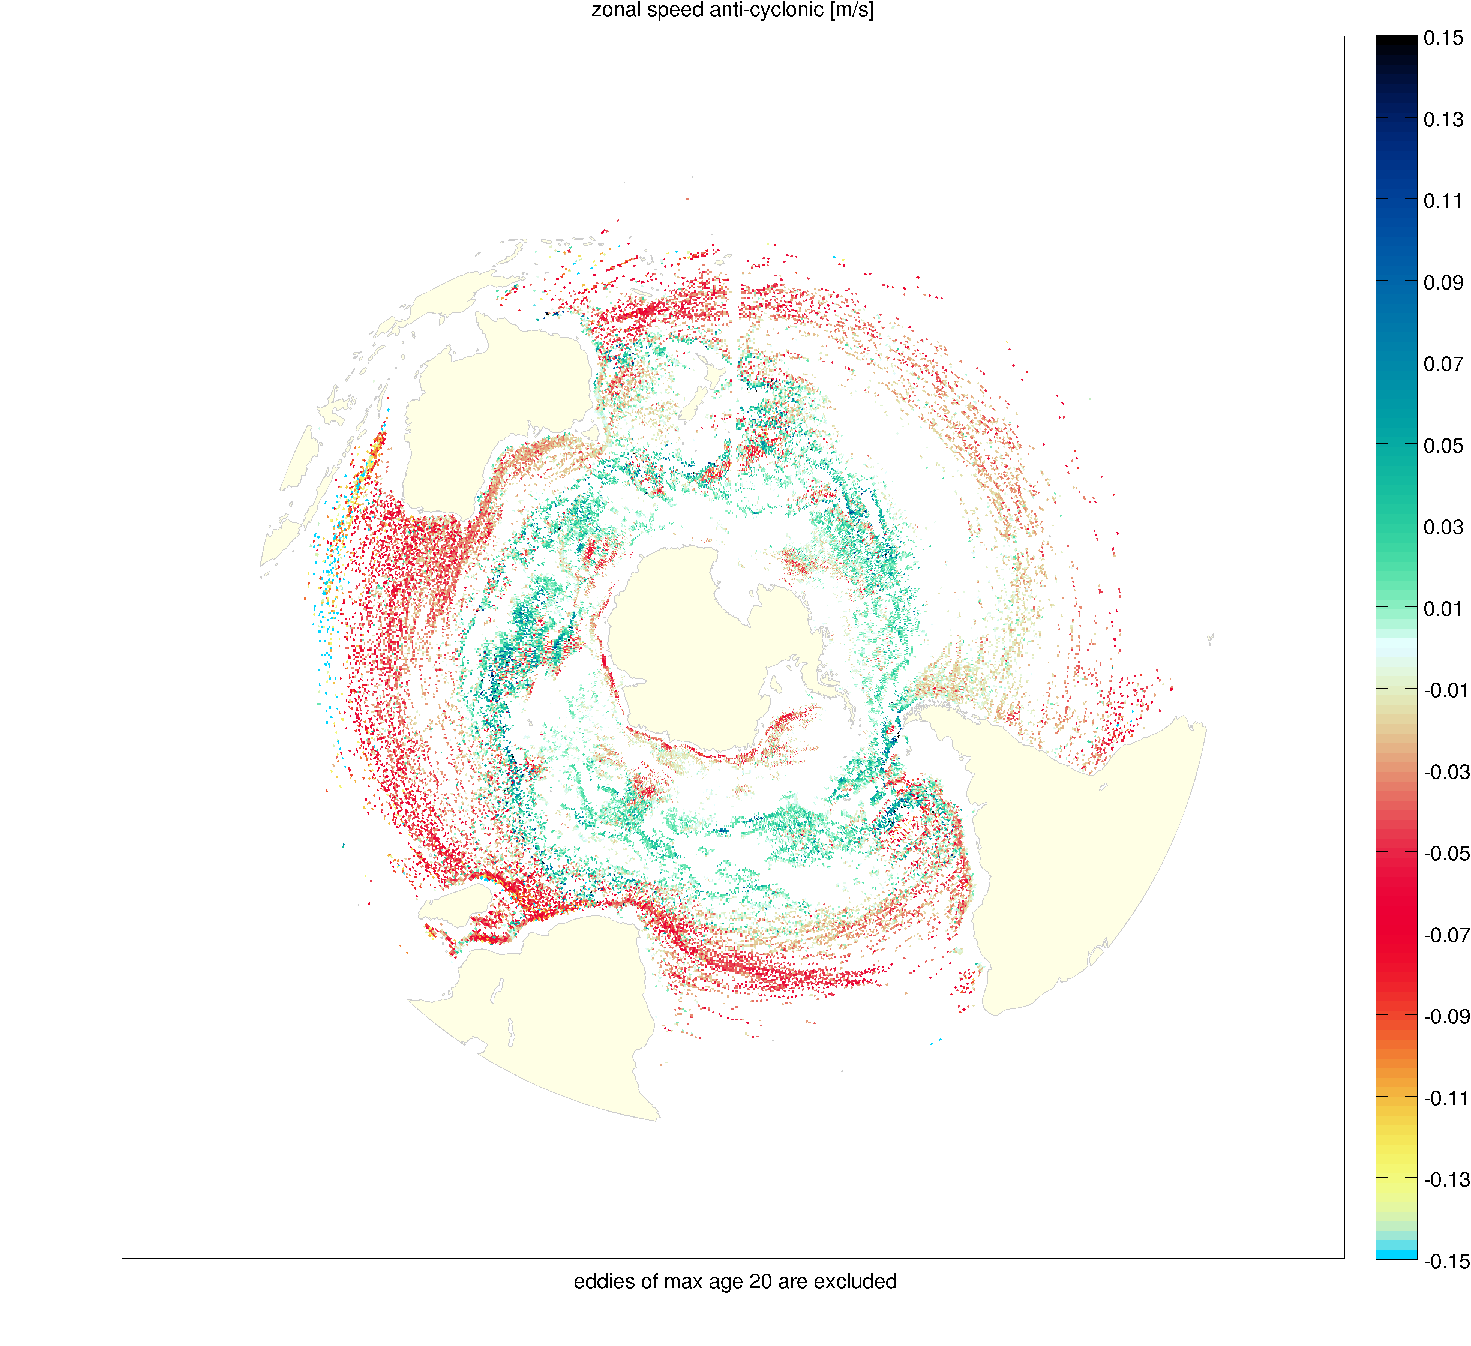
\includegraphics[width=.8\textwidth]{ACC.pdf}
 % ACC.pdf: 706x646 pixel, 72dpi, 24.91x22.79 cm, bb=0 0 706 646
 \caption{ACC drift speeds}
 \label{fig:ACC}
\end{figure}

\begin{figure}
 \centering
 \includegraphics[width=.9\textwidth]{age_tracks.pdf}
 % age_tracks.pdf: 923x1155 pixel, 72dpi, 32.56x40.75 cm, bb=0 0 923 1155
  \caption{note: scales are wrong! shifted by 20 respective 50 days...}
  \label{fig:age_tracks}
\end{figure}

\begin{figure}
 \centering
 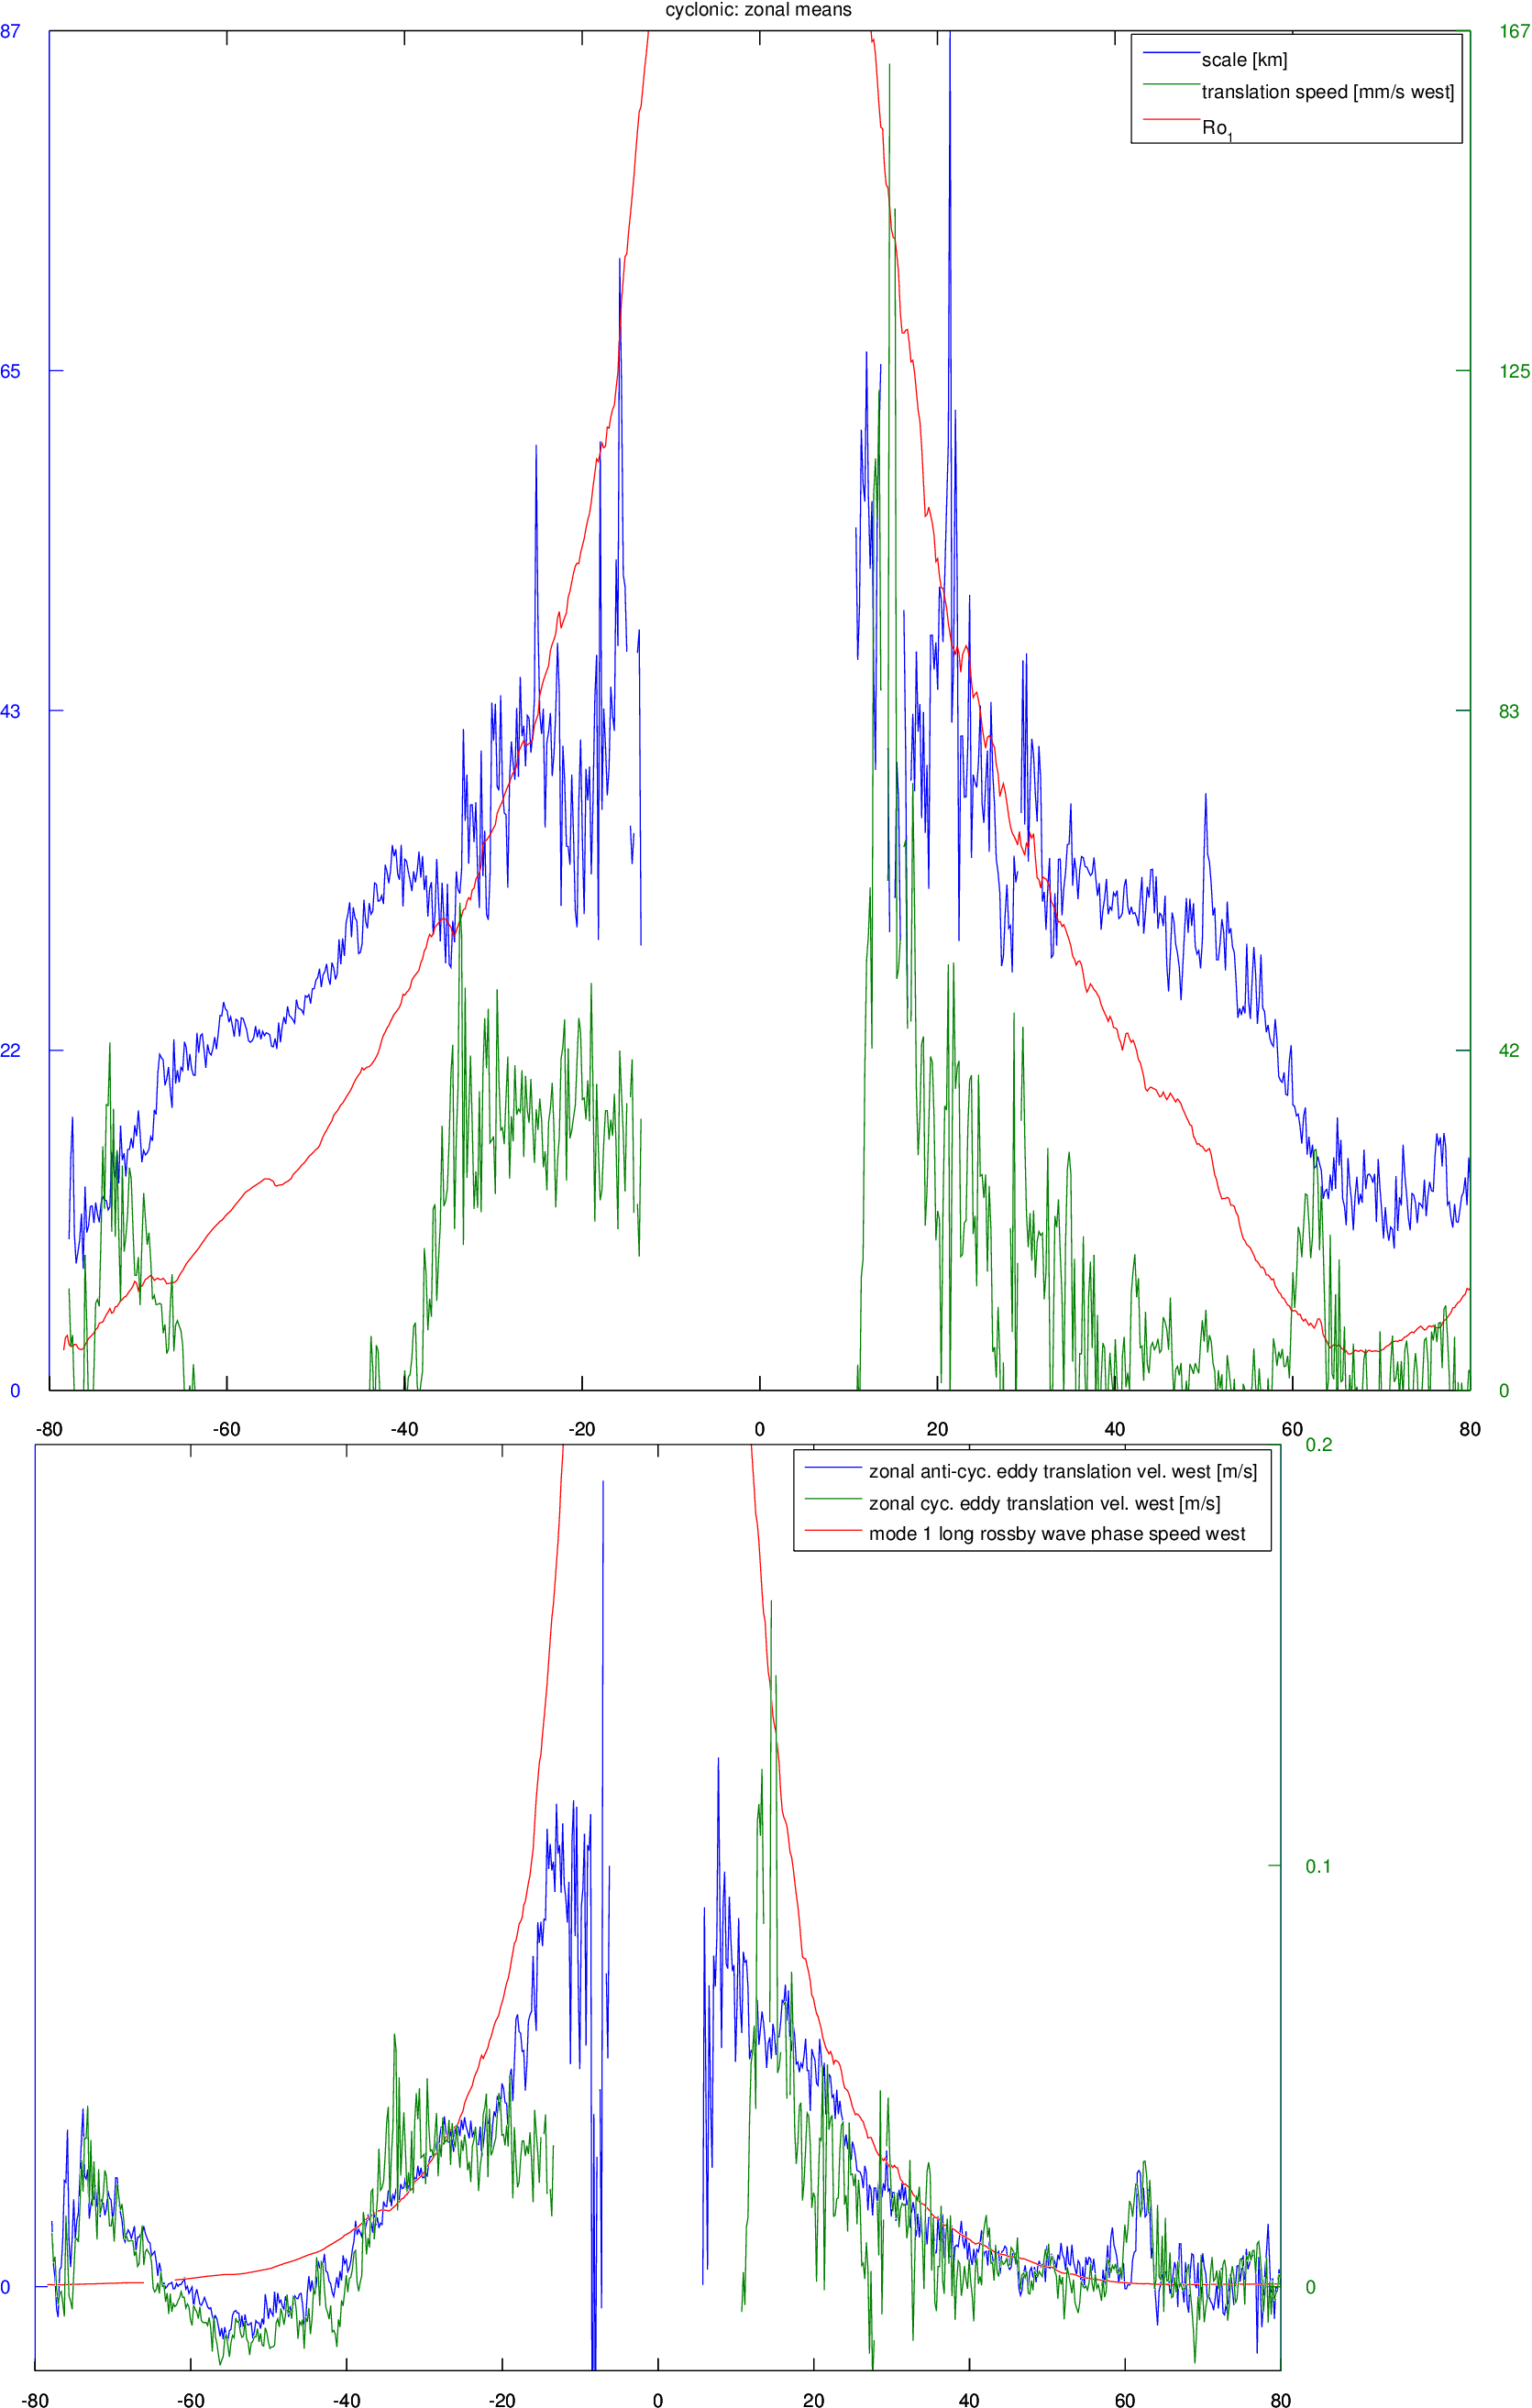
\includegraphics[height=.8\textheight]{cyc_speeds.pdf}
 % cyc_speeds.pdf: 802x1261 pixel, 72dpi, 28.29x44.49 cm, bb=0 0 802 1261
 \label{fig:cyc_speeds}
\end{figure}

% 
% 
% 
% \end{appendices}
% %
% %
% \backmatter
% \newgeometry{left=4cm, right=4cm, top=3cm, bottom=3cm}
% %
% %
% %
%  \Declaration{
I, \authornames, declare that this thesis titled, '\ttitle' and the work presented in it are my own. I confirm that:

\begin{itemize}
\item[\tiny{$\blacksquare$}] This work was done wholly or mainly while in candidature for a research degree at this University.
\item[\tiny{$\blacksquare$}] Where any part of this thesis has previously been submitted for a degree or any other qualification at this University or any other institution, this has been clearly stated.
\item[\tiny{$\blacksquare$}] Where I have consulted the published work of others, this is always clearly attributed.
\item[\tiny{$\blacksquare$}] Where I have quoted from the work of others, the source is always given. With the exception of such quotations, this thesis is entirely my own work.
\item[\tiny{$\blacksquare$}] I have acknowledged all main sources of help.
\item[\tiny{$\blacksquare$}] Where the thesis is based on work done by myself jointly with others, I have made clear exactly what was done by others and what I have contributed myself.\\
\end{itemize}

Signed:\\
\rule[1em]{25em}{0.5pt} % This prints a line for the signature

Date:\\
\rule[1em]{25em}{0.5pt} % This prints a line to write the date
}

\clearpage % Start a new page

%  \setstretch{1.3} % Reset the line-spacing to 1.3 for body text (if it has changed)
\acknowledgements{\addtocontents{toc}{\vspace{1em}} % Add a gap in the Contents, for aesthetics

The acknowledgements and the people to thank go here, don't forget to include your project advisor\ldots
}
\clearpage % Start a new page

% % 
$a$: amplitude\\
$\rG$: \textit{Gaussian radius} \ie twice Gaussian \textit{std} \\
$H$: Gaussian amplitude\\
$A$: determined area\\
$r$: determined radius\\
with $A=\pi r^2$ and $V=2\pi\sigma^2$
\begin{align}
 H-a 
&= 
H \exp \left( -\frac{A}{2 \pi \left( \rG/2 \right)^2}  \right) \\ 
\end{align}
and

\begin{align}
 H-a 
&= 
H \exp \left( -\frac{A}{2 \pi \left( \rG/2 \right)^2}  \right) \\
  1-a/H 
&= 
 \exp \left( -\frac{2A}{\pi \rG^2}  \right) \\
  \pi \rG^2
&= 
  \left( -\frac{2A}{\ln \l 1-a/H \r }  \right) \\
 \rG
&= 
 \sqrt{-\frac{2A}{\pi \ln \l 1-a/H \r }}  \\
\end{align}
















with $\gamma=-\frac{1}{2 \sigma^2} $ \\
\begin{align}
g(x,y)= h \exp \left(\gamma \left(  y^2 + x^2 \right) \right)
\end{align}

\begin{align}
V =  \int_{-r}^{r}\int_{-r}^{r} g \dint{x}\dint{y}
\end{align}

\begin{align}
	\lambda(r) &= \frac{V}{A^{1.5}}\\
		&= 
	\frac{  \int_{-r}^{r}\int_{-r}^{r} g \dint{x}\dint{y}}
{ \left(   \pi r^2  \right)^{3/2}}\\
&=
 \left(r \sqrt{\pi}    \right)^{-3}
 \int_{-r}^{r}\int_{-r}^{r} g \dint{x}\dint{y}\\
&=
   \left(r \sqrt{\pi}    \right)^{-3}
\int_{-r}^{r} \left[   \frac{  g }{ 2\gamma x} \right]^{r}_{-r} \dint{y}\\
&=
 \left(r \sqrt{\pi}    \right)^{-3}
\int_{-r}^{r} 
 \frac{  \exp \left(\gamma \left(  y^2 + r^2 \right) \right)   }{ 2 \gamma r}
-  \frac{  \exp \left(\gamma \left(  y^2 + r^2 \right) \right)   }{- 2 \gamma r}
  \dint{y}\\
&=
 \left(r \sqrt{\pi}    \right)^{-3}
\int_{-r}^{r} 
 \exp \left(\gamma \left(  y^2 + r^2 \right) \right) 
\left( 
 \frac{  1 }{  \gamma r}
 \right)
  \dint{y}\\
&=
\left( \gamma r^4 \pi^{3/2}  \right)^{-1}
\int_{-r}^{r} g(r,y) \dint{y}\\
&=
\left( \gamma r^4 \pi^{3/2}  \right)^{-1}
\int_{-r}^{r} g(r,y) \dint{y}\\
&=
h\left( \gamma r^4 \pi^{3/2}  \right)^{-1}
 \frac{  \exp \left(\gamma \left(  y^2 + r^2 \right) \right)  }{ \gamma r}  \\
&=
h\left( \gamma^2 r^5 \pi^{3/2}  \right)^{-1}
 g(r,r)   \\
&=
h^2 \pi^{2/3}
\frac
{
\exp \left(\gamma \left(  2 r^2 \right) \right)
}
{
\gamma^2 r^5 
}
\end{align}

\begin{align}
&= 
\frac
{
\exp \left( 2 r^2  \right)
}
{
r^5 
}
\end{align}
% 
% 
% $A_{\circ}$ : area of circle with equal perimeter
% %%....................................................................
% \begin{align}
% 	q_a
% 	&=
% 	\frac{A}{A_{\circ}}  \\
% 	&=
% 	\frac{A}{   \pi r_{\circ}^2   }  \\
% 	&=
% 	 \frac{A}{   \pi \left( \frac{p}{2 \pi} \right)^2   }  \\
% 	&=
% 	4 \pi\frac{A}{   p^2   }  
% \end{align}
% %%....................................................................
% $p_{\circ}$ : perimeter of circle with equal area
% %%....................................................................
% \begin{align}
% 	q_s
% 	&=
% 	\frac{p_{\circ}}{p}  \\
% 	&=
% 	\frac{ 2 \pi r_{\circ} }{p}  \\
% 	&=
% 	\frac{ 2 \pi \sqrt{ A/\pi  }}{p}  \\
%  	&=
% 	\frac{ 2  \sqrt{\pi A }}{p} \\
% &=
% \sqrt{q_a}
% \end{align}
% %%....................................................................
% 
% 
% 
% \begin{figure}[!ht]
% 	\centering
% 	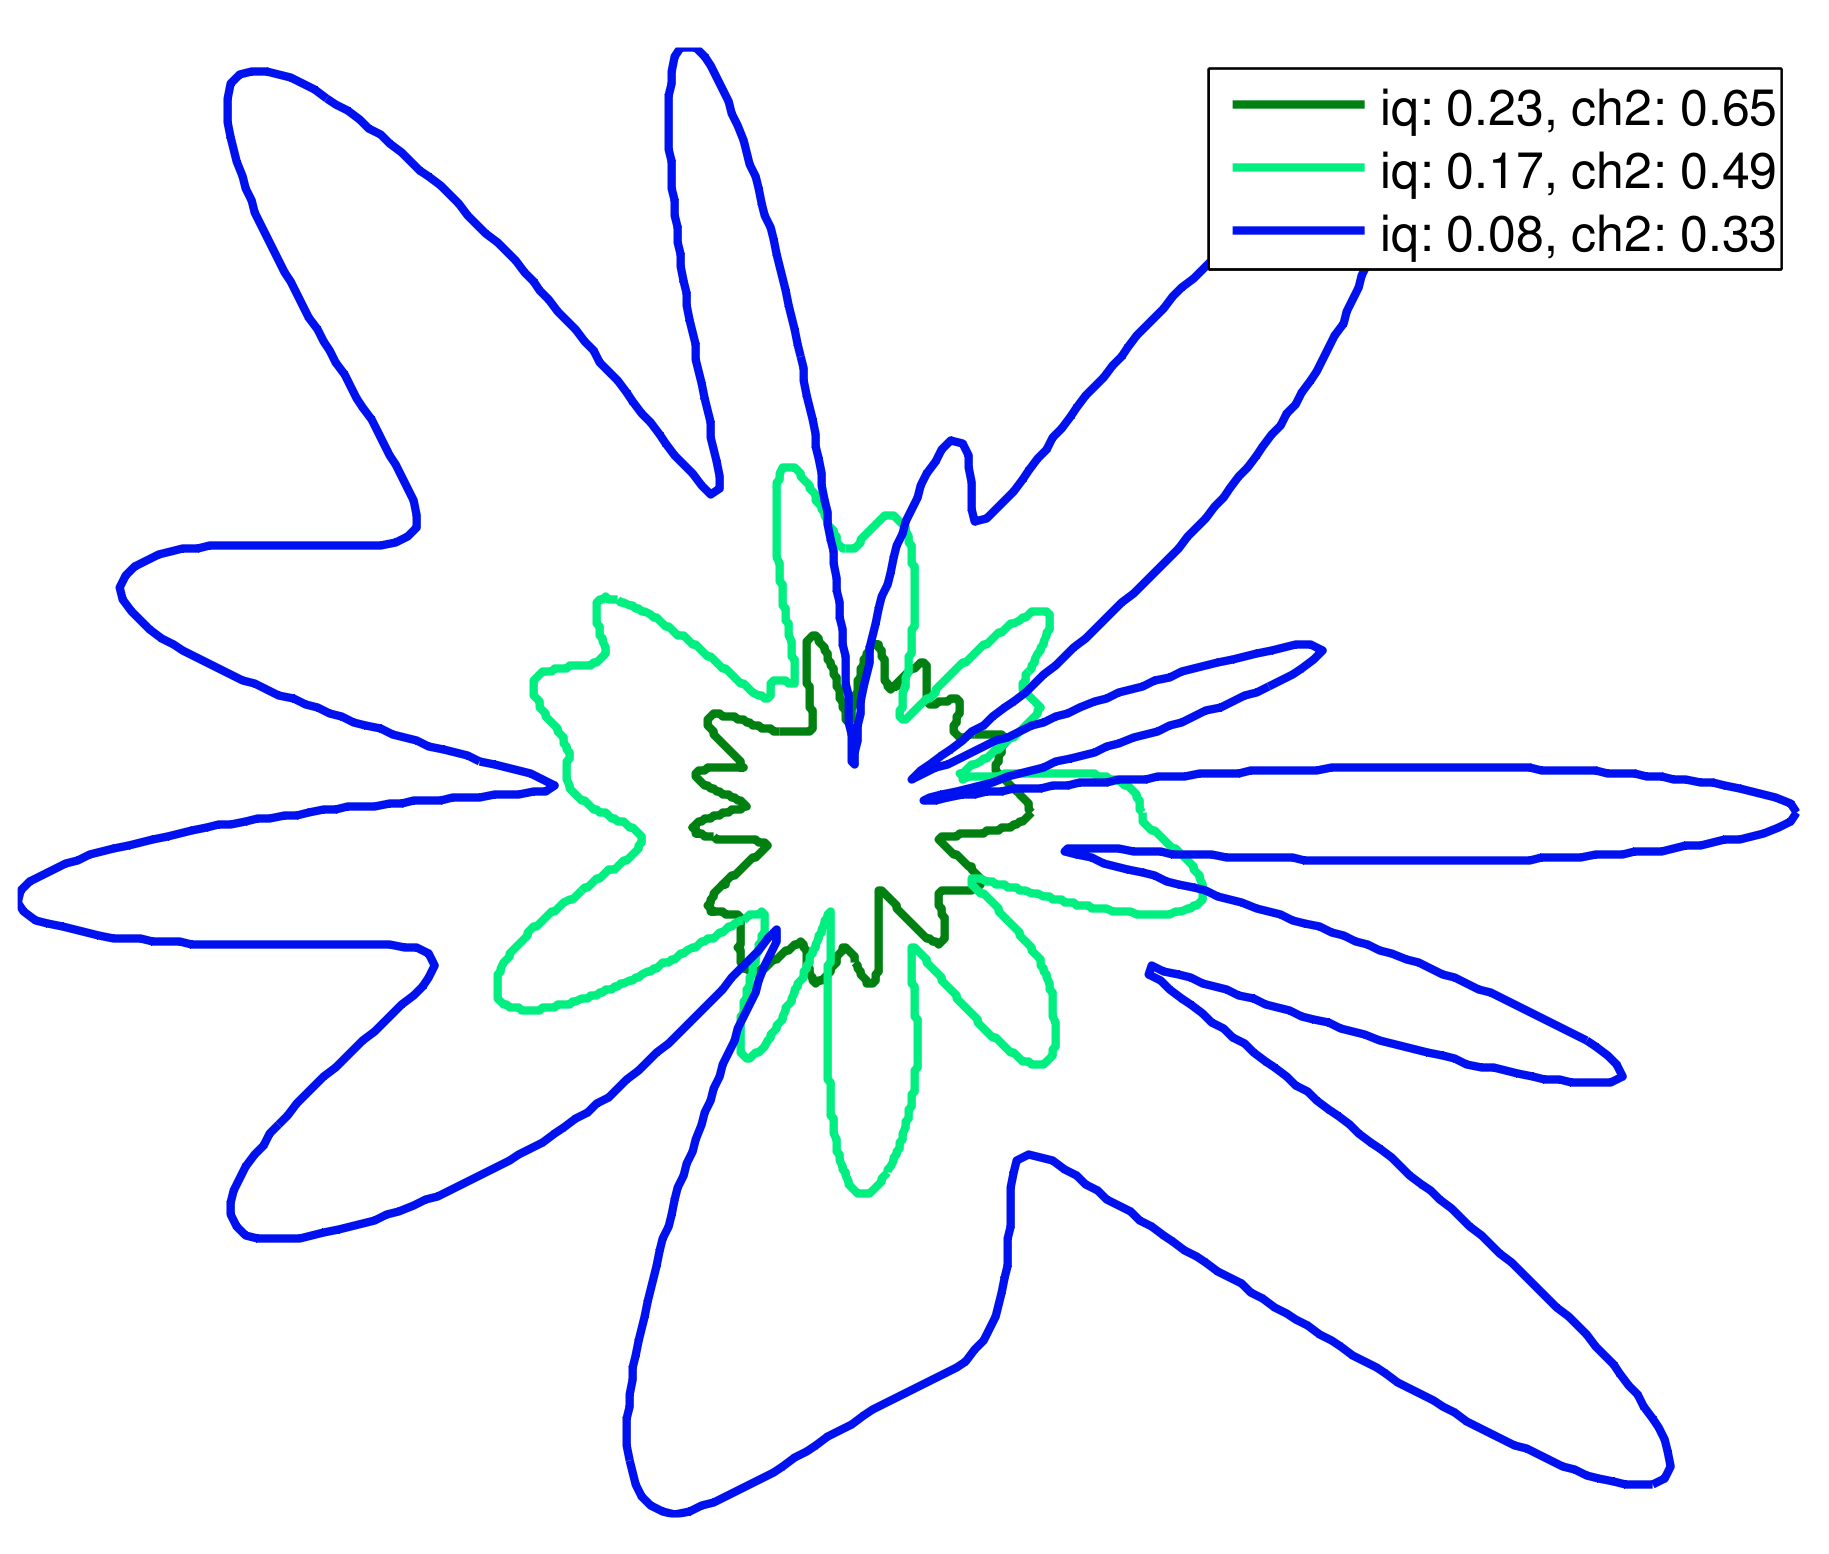
\includegraphics[scale=.7]{./huh.png}
% 	% huh.png: 1829x1554 pixel, 300dpi, 15.49x13.16 cm, bb=0 0 439 373
% \end{figure}
% 
% 
% 
% chelton:
% %%....................................................................
% \begin{align}
% h_a
% &=
% \frac{d}{\mu}
% \end{align}
% with
% \begin{equation}
% \mu=
% \begin{cases}
% 	400km &; \norm{\phi} > 25^{\circ}  \\
% 	\left( 800 \frac{\left( 25-\norm{\phi}  \right)}{25} + 400  \right) km &; \norm{\phi} \leqslant 25^{\circ}
% \end{cases}
% \end{equation}
% %%....................................................................
% alternative
% %%....................................................................
% \begin{align}
% h_b
% &=
% 4 \pi \frac{A}{ \left( \pi d  \right)^2}  \\
% &=
% 4 \frac{A}{ \pi d^2}  
% \end{align}
% %%....................................................................
% 
% 
% 



Integrating \eqref{eq:Emech1} over a closed Volume with standard boundary conditions yields a Eularian equation
for the change in total mechanical energy of the domain (Note that the advection term does just that - \textit{advect}.
It has no contribution to the total change of energy).
%%....................................................................
\begin{equation}\begin{split}
\frac{1}{2}\left(
	\int_{V} \frac{\partial \vec{u}^2}{\partial t}  \; \mathrm{d}V
  +
	\int_{V} \vec{u} \cdot \grad \vec{u}^2 \; \mathrm{d}V
	\right)
	&=
	\int_{V} \vec{u}\cdot \nu  \vec{\nabla}^{2} \vec{u}  \; \mathrm{d}V \\
	%%--------------------------------------------------------------------
	\int_{V} \frac{\partial \Em}{\partial t}  \; \mathrm{d}V
	&=
	\int_{V} \nu\left(
	\frac{1}{2}\grad^2 \vec{u}^2 - \norm{\grad \vec{u}}^2
	\right)  \; \mathrm{d}V
\end{split}\end{equation}
%%....................................................................


%%####################################################################
%%####################################################################


%%####################################################################
%%####################################################################


\section{2D-Turbulence}
oiug
\subsection{Aspect Ratio}
\subsection{Enstrophy Conservation}
Without a third dimension, vorticity can no longer be altered by stretching or tilting.
\eqref{eq:vort2} then reduces to:
\begin{equation}\begin{split}
	\frac{D \omega_{a}}{D t}
	&=
	\nu \grad^{2} \omega
\end{split}\end{equation}
In other words, in absence of friction, besides energy, now also vorticity is materially conserved.
\subsubsection{}


\begin{equation}\begin{split}
	\int_A \omega \frac{D \omega_{a}}{D t}\; \mathrm{d}A
	&=
	\nu\int_A  \omega \grad^{2} \omega\; \mathrm{d}A\\
	\frac{\partial \Enstro}{\partial t}
	=
	\frac{\partial }{2\partial t} \int_A \omega^2 \; \mathrm{d}A
	&=
	\nu\int_A \frac{1}{2}\grad^{2} \omega^{2} - \norm{\grad \omega}^2  \; \mathrm{d}A \\
	&=
	\frac{\nu}{2}\oint_A \grad \omega^{2} \cdot \mathrm{d}\vec{s}
	- \int_A\norm{\grad \omega}^2  \; \mathrm{d}A \label{eq:enst1}	\\
\end{split}\end{equation}


\begin{equation}\begin{split}
	\int_A \omega \frac{D \omega_{a}}{D t}\; \mathrm{d}A
	&=
	\nu\int_A  \omega \grad^{2} \omega\; \mathrm{d}A\\
	\frac{\partial \Enstro}{\partial t}
	=
	\frac{\partial }{2\partial t} \int_A \omega^2 \; \mathrm{d}A
	&=
	\nu\int_A \omega  \frac{\partial }{\partial x_i} \vec{e}_i \frac{\partial  \omega}{\partial x_i} \vec{e}_i\; \mathrm{d}A \\
	&=
	\nu\int_A \omega  \frac{\partial^2  \omega}{\partial x_i^2} \; \mathrm{d}A \\
	%%--------------------------------------------------------------------
	&=
	\nu\int_A \frac{1}{2} \frac{\partial^2 \omega^2 }{\partial x_i^2}  - \left(\frac{\partial  \omega}{\partial x_i} \right)^2 \; \mathrm{d}A \label{eq:enst1}
\end{split}\end{equation}
If we now consider an infinite domain with fading $\vec{u}$ away from the center,
the first RHS-term of \eqref{eq:enst1} vanishes, leaving:
\begin{equation}\begin{split}
	\frac{\partial \Enstro}{\partial t}
	&=
	- \int_A \nu\left(\frac{\partial  \omega}{\partial x_i} \right)^2 \; \mathrm{d}A \\
	&=
	- \int_A \nu\norm{ \grad \omega}^2 \; \mathrm{d}A
\end{split}\end{equation}



In 2 dimensions enstrophy can also be rewritten as follows:
%%....................................................................
\begin{equation}\begin{split}
\Enstro
&=
\int_{V} \norm{\vec{\omega}}^{2}  \; \mathrm{d}V\\
&=
\int_{V} \omega^{2}  \; \mathrm{d}V\\
&=
\int_{V} \left( \frac{\partial v}{\partial x} - \frac{\partial u}{\partial y} \right)^2  \; \mathrm{d}V\\
&=
\int_{V} \left(\frac{\partial v}{\partial x}\right)^2
-2\frac{\partial v}{\partial x} \frac{\partial u}{\partial y}
+ \left(\frac{\partial u}{\partial y} \right)^2  \; \mathrm{d}V\\
&=
\int_{V} \left(\frac{\partial v}{\partial x}\right)^2
+ \left(\frac{\partial u}{\partial y} \right)^2
-2\frac{\partial v}{\partial x} \frac{\partial u}{\partial y}
+ \left( \div \vec{u} \right)^2
  \; \mathrm{d}V\\
&=
\int_{V} \left(\frac{\partial v}{\partial x}\right)^2
+ \left(\frac{\partial u}{\partial y} \right)^2
+\left(\frac{\partial v}{\partial y}\right)^2
+ \left(\frac{\partial u}{\partial x} \right)^2
  \; \mathrm{d}V\\
  &=
\int_{V}
\norm{\grad \vec{u}}^2
\; \mathrm{d}V\\
  &=
\int_{V}
\frac{1}{2} \grad^2 \vec{u}^2 -\vec{u} \cdot \grad^2 \vec{u}
\; \mathrm{d}V\\
  &=
\frac{1}{2}\oint_{A}   \grad \vec{u}^2 \cdot  \; \mathrm{d}\vec{s}
-\int_{V}\vec{u} \cdot \grad^2 \vec{u}  \; \mathrm{d}V\\
  &=
\int_{V}
-\vec{u} \cdot \grad^2 \vec{u}
\; \mathrm{d}V\\
\end{split}\end{equation}
\textit{...under appropriate boundary conditions} WHY???\\
%%--------------------------------------------------------------------
combinging ... and ... reveals the coupling	that energy dissipation is proportional to the total enstrophy of the system.
And that


\begin{equation}\begin{split}
	\int_{V}\frac{\partial E_{m}}{\partial t} \; \mathrm{d}V
	&=
	-\nu \int_{V} \norm{\vec{\omega}}^{2}  \; \mathrm{d}V \\
	%%--------------------------------------------------------------------
	&=
	-\nu \Enstro\\
	\int_{V}\frac{\partial E_{m}}{\partial t} \; \mathrm{d}V
	&=
	\grad^{2} \frac{D \Enstro}{D t}
\end{split}\end{equation}



\chapter{junk}



%%....................................................................
\begin{equation}\begin{split}
	\frac{\partial \enstro}{\partial t}
	+
	\vec{u} \cdot \grad \enstro
	&=
	-\nu \grad^{2} \enstro\\
	\frac{\partial \norm{\grad \vec{u}}^{2}}{\partial t}
	+
	\vec{u} \cdot \grad \norm{\grad \vec{u}}^{2}
	&=
	-\nu \grad^{2} \norm{\grad \vec{u}}^{2}\\
	\frac{\partial }{\partial t} \left(\frac{\partial u_{i}}{\partial x_{j}}\right)^{2}
	+
	u_{k}  \frac{\partial}{\partial x_{k}} \left(\frac{\partial u_{i}}{\partial x_{j}}\right)^{2}
	&=
	-\nu \grad^{2}  \left(\frac{\partial u_{i}}{\partial x_{j}}\right)^{2}\\
\end{split}\end{equation}


\begin{equation}\begin{split}
	\frac{\partial \enstro}{\partial t}
&=
	-
	\vec{u} \cdot \grad \enstro
	-\nu \grad^{2} \enstro{}
	+\vec{\omega}_{a}\cdot \left( \vec{\vec{\omega}_{a}} \cdot \grad \right) \vec{\vec{u}}\\
&\sim-
	\frac{U^{3}}{L^{3}}
	- \frac{\nu U^{2}}{L^{4}}
	+ \frac{U^{3}}{L^{3}}\\
\end{split}\end{equation}

\begin{equation}\begin{split}
	\frac{\partial E_{m}}{\partial t}
&\sim{}
-	\frac{U^{3}}{L}
	- \frac{\nu U^{2}}{L^{2}} \\
	&\sim
	\frac{\partial \enstro}{\partial t} L^{2}
\end{split}\end{equation}







% % \chapter{UNSORTED}

\begin{itemize}

\item
thought:\\ L - magnitude\\ T(lifetime) ~ cascade-rate of baroclin energy \cite{larichev1995eddy} \\ U - spatial distro



\end{itemize}
 \todoil{SORT}
%  \listoftodos
 \bibliographystyle{authordate1}
% %\bibliographystyle{plainnat}
 \bibliography{/home/niko/documents/library.bib}

\end{document}











